%%
%% This is file `sample-manuscript.tex',
%% generated with the docstrip utility.
%% 
%% The original source files were:
%%
%% samples.dtx  (with options: `all,proceedings,bibtex,manuscript')
%% 
%% IMPORTANT NOTICE:
%% 
%% For the copyright see the source file.
%% 
%% Any modified versions of this file must be renamed
%% with new filenames distinct from sample-manuscript.tex.
%% 
%% For distribution of the original source see the terms
%% for copying and modification in the file samples.dtx.
%% 
%% This generated file may be distributed as long as the
%% original source files, as listed above, are part of the
%% same distribution. (The sources need not necessarily be
%% in the same archive or directory.)
%%
%%
%% Commands for TeXCount
%TC:macro \cite [option:text,text]
%TC:macro \citep [option:text,text]
%TC:macro \citet [option:text,text]
%TC:envir table 0 1
%TC:envir table* 0 1
%TC:envir tabular [ignore] word
%TC:envir displaymath 0 word
%TC:envir math 0 word
%TC:envir comment 0 0
%%
%% The first command in your LaTeX source must be the \documentclass
%% command.
%%
%% For submission and review of your manuscript please change the
%% command to \documentclass[manuscript, screen, review]{acmart}.
%%
%% When submitting camera ready or to TAPS, please change the command
%% to \documentclass[sigconf]{acmart} or whichever template is required
%% for your publication.
%%
%%
\documentclass[manuscript,review]{acmart}
%%
%% \BibTeX command to typeset BibTeX logo in the docs
\AtBeginDocument{%
  \providecommand\BibTeX{{%
    Bib\TeX}}}

\usepackage{multirow}
\usepackage{booktabs}
\usepackage{tabularx}
\usepackage{array}
\usepackage{makecell}
\usepackage{graphicx}
\usepackage[table]{xcolor}
\usepackage{threeparttable}
\usepackage{rotating}
\usepackage{adjustbox}
\usepackage{pdflscape}
\usepackage{tikz}
\usetikzlibrary{positioning,calc}
\usepackage{adjustbox}
\usepackage{pgfplots}
\pgfplotsset{compat=1.18}
\usepackage{subcaption}

\usepackage{longtable}
\usepackage{ragged2e}

\usepackage{amsmath} 



% =========================
% Colors
% =========================
\definecolor{headergray}{HTML}{BFBFBF}
\definecolor{rowgrayA}{HTML}{F7F7F7}
\definecolor{rowgrayB}{HTML}{EFEFEF}
\definecolor{rowgrayC}{HTML}{E5E5E5}

\definecolor{bestblue}{HTML}{8EB9D3}
\definecolor{secondblue}{HTML}{B7D7E8}
\definecolor{thirdblue}{HTML}{DCEFF7}

\newcommand{\best}[1]{\cellcolor{bestblue}{\boldmath\bfseries #1}}
\newcommand{\second}[1]{\cellcolor{secondblue}{\boldmath\bfseries #1}}
\newcommand{\third}[1]{\cellcolor{thirdblue}{\boldmath\bfseries #1}}


%% Rights management information.  This information is sent to you
%% when you complete the rights form.  These commands have SAMPLE
%% values in them; it is your responsibility as an author to replace
%% the commands and values with those provided to you when you
%% complete the rights form.
\setcopyright{acmlicensed}
\copyrightyear{2018}
\acmYear{2018}
\acmDOI{XXXXXXX.XXXXXXX}
%% These commands are for a PROCEEDINGS abstract or paper.
\acmConference[Conference acronym 'XX]{Make sure to enter the correct
  conference title from your rights confirmation email}{June 03--05,
  2018}{Woodstock, NY}
%%
%%  Uncomment \acmBooktitle if the title of the proceedings is different
%%  from ``Proceedings of ...''!
%%
%%\acmBooktitle{Woodstock '18: ACM Symposium on Neural Gaze Detection,
%%  June 03--05, 2018, Woodstock, NY}
\acmISBN{978-1-4503-XXXX-X/2018/06}


%%
%% Submission ID.
%% Use this when submitting an article to a sponsored event. You'll
%% receive a unique submission ID from the organizers
%% of the event, and this ID should be used as the parameter to this command.
%%\acmSubmissionID{123-A56-BU3}

%%
%% For managing citations, it is recommended to use bibliography
%% files in BibTeX format.
%%
%% You can then either use BibTeX with the ACM-Reference-Format style,
%% or BibLaTeX with the acmnumeric or acmauthoryear sytles, that include
%% support for advanced citation of software artefact from the
%% biblatex-software package, also separately available on CTAN.
%%
%% Look at the sample-*-biblatex.tex files for templates showcasing
%% the biblatex styles.
%%

%%
%% The majority of ACM publications use numbered citations and
%% references.  The command \citestyle{authoryear} switches to the
%% "author year" style.
%%
%% If you are preparing content for an event
%% sponsored by ACM SIGGRAPH, you must use the "author year" style of
%% citations and references.
%% Uncommenting
%% the next command will enable that style.
%%\citestyle{acmauthoryear}


%%
%% end of the preamble, start of the body of the document source.
\begin{document}

%%
%% The "title" command has an optional parameter,
%% allowing the author to define a "short title" to be used in page headers.
\title{EHR-Based Medication Recommendation: A Stage-Oriented Survey and Unified Benchmark}

%%
%% The "author" command and its associated commands are used to define
%% the authors and their affiliations.
%% Of note is the shared affiliation of the first two authors, and the
%% "authornote" and "authornotemark" commands
%% used to denote shared contribution to the research.
\author{Yeguang Zhen}
\authornote{Contributed equally to this research.}
\affiliation{
    \institution{Key Laboratory of Computing Power Network and Information Security, Ministry of Education, Shandong Computer Science Center (National Supercomputer Center in Jinan), Qilu University of Technology (Shandong Academy of Sciences); Shandong Provincial Key Laboratory of Computing Power Internet and Service Computing, Shandong Fundamental Research Center for Computer Science}
    \country{China}
}
\email{zhenyeguang92@gmail.com}

% \orcid{1234-5678-9012}
\author{Shoujin Wang}
\email{Shoujin.Wang@uts.edu.au}
\authornotemark[1]
\affiliation{%
  \institution{Data Science Institute, University of Technology Sydney}
  \city{Sydney}
  \country{Australia}
}

\author{Yishuo Li}
\affiliation{
  %\institution{Key Laboratory of Computing Power Network and Information Security, Ministry of Education, Shandong Computer Science Center (National Supercomputer Center in Jinan), Qilu University of Technology (Shandong Academy of Sciences); Shandong Provincial Key Laboratory of Computing Power Internet and Service Computing, Shandong Fundamental Research Center for Computer Science}
  \institution{Qilu University of Technology (Shandong Academy of Sciences)}
  \city{Jinan}
  \country{China}
}

\author{Liang Hu}
\affiliation{
  \institution{Department of Computer Science and Technology, Tongji University}
  \city{Shanghai}
  \country{China}
}

\author{Defu Lian}
\affiliation{
  \institution{School of Computer Science and Technology, University of Science and Technology of China}
  \city{Hefei}
  \country{China}
}

\author{Cong Wang}
\affiliation{
  %\institution{Key Laboratory of Computing Power Network and Information Security, Ministry of Education, Shandong Computer Science Center (National Supercomputer Center in Jinan), Qilu University of Technology (Shandong Academy of Sciences); Shandong Provincial Key Laboratory of Computing Power Internet and Service Computing, Shandong Fundamental Research Center for Computer Science}
  \institution{Qilu University of Technology (Shandong Academy of Sciences)}
  \city{Jinan}
  \country{China}
}

\author{Wenpeng Lu}
\authornote{Corresponding Author.}
\affiliation{%
  %\institution{Key Laboratory of Computing Power Network and Information Security, Ministry of Education, Shandong Computer Science Center (National Supercomputer Center in Jinan), Qilu University of Technology (Shandong Academy of Sciences); Shandong Provincial Key Laboratory of Computing Power Internet and Service Computing, Shandong Fundamental Research Center for Computer Science}
  \institution{Qilu University of Technology (Shandong Academy of Sciences)}
  \city{Jinan}
  \country{China}
}
\email{wenpeng.lu@qlu.edu.cn}


%%
%% By default, the full list of authors will be used in the page
%% headers. Often, this list is too long, and will overlap
%% other information printed in the page headers. This command allows
%% the author to define a more concise list
%% of authors' names for this purpose.
% renewcommand{\shortauthors}{Trovato et al.}

%%
%% The abstract is a short summary of the work to be presented in the
%% article.
\begin{abstract}
% 临时版本
% Medication recommendation aims to assist physicians in generating accurate, personalized, and safe medication combinations from electronic health records (EHRs). Recent studies have largely followed an EHR-based paradigm, while progressively incorporating longitudinal patient histories, drug-drug interaction constraints, molecular structures, drug knowledge graphs, causal learning, and PLM/LLM-based techniques to improve recommendation accuracy, safety, and clinical reasoning. However, the rapid growth of this field has made existing methods difficult to systematically organize and fairly compare, due to differences in clinical signals, knowledge sources, preprocessing procedures, medication granularities, data splitting protocols, and evaluation metrics. 
% This survey presents a stage-oriented review and unified empirical evaluation of medication recommendation systems. We organize existing studies into three functional stages: patient representation, medication representation, and medication recommendation, clarifying the roles of different techniques in the EHR-based recommendation pipeline. We further construct a unified benchmark across multiple public EHR datasets and medication granularities to compare representative models under consistent experimental settings. Based on this benchmark, we analyze how dataset characteristics, medication granularity, model design, and safety constraints affect recommendation performance. Finally, we discuss open challenges and future directions for medication recommendation.

Medication recommendation seeks to support clinicians in selecting appropriate medication sets from longitudinal electronic health records (EHRs) while balancing predictive accuracy and medication safety. 
Recent studies have extended the EHR-based paradigm through longitudinal modeling, drug-drug interaction knowledge, molecular and graph-based drug representations, causal learning, and PLM/LLM-assisted methods. 
However, the field remains difficult to navigate and evaluate because existing studies differ substantially in clinical inputs, external knowledge sources, preprocessing pipelines, medication coding granularities, data-splitting protocols, and evaluation metrics. 
This survey provides a stage-oriented taxonomy and a unified empirical benchmark for EHR-based medication recommendation. We organize existing methods into three functional stages: patient representation, medication representation, and medication recommendation, clarifying where different techniques contribute within the end-to-end recommendation pipeline. 
We then benchmark representative methods across multiple public EHR datasets and medication granularities under consistent preprocessing, splitting, and evaluation protocols. The resulting analyses examine how dataset heterogeneity, medication granularity, model design, and safety constraints affect recommendation accuracy, drug-drug interaction risk, cross-dataset generalization, and long-tail performance. Finally, we identify open challenges in effective patient-history utilization, rare-medication recommendation, controllable safety-accuracy trade-offs, and trustworthy LLM-assisted medication recommendation.

\end{abstract}

%%
%% The code below is generated by the tool at http://dl.acm.org/ccs.cfm.
%% Please copy and paste the code instead of the example below.
%%
\begin{CCSXML}
<ccs2012>
 <concept>
  <concept_id>10002944.10011122</concept_id>
  <concept_desc>General and reference~Surveys and overviews</concept_desc>
  <concept_significance>500</concept_significance>
 </concept>
</ccs2012>
\end{CCSXML}

\ccsdesc[500]{Surveys and overviews}
%%
%% Keywords. The author(s) should pick words that accurately describe
%% the work being presented. Separate the keywords with commas.
\keywords{Medication Recommendation, Healthcare Benchmarking}

% \received{20 February 2007}
% \received[revised]{12 March 2009}
% \received[accepted]{5 June 2009}

%%
%% This command processes the author and affiliation and title
%% information and builds the first part of the formatted document.
\maketitle
% \clearpage

\section{Introduction}


% Recommender systems have become an important technique for mitigating information overload and supporting personalized decision-making by modeling user preferences, contextual factors, and historical interactions. 
% With the rapid digitization of healthcare, this paradigm has been increasingly extended to clinical settings, where electronic health records (EHRs) offer rich longitudinal information for data-driven decision support. 
% A prominent and safety-critical application is medication recommendation, which focuses on suggesting appropriate medications based on patients’ clinical conditions and medical histories. 
% In real-world clinical practice, patients often present with multiple diseases and require combination therapies. Physicians must therefore consider heterogeneous clinical evidence, including diagnoses, procedures, laboratory results, historical prescriptions, comorbidities, contraindications, and potential drug-drug interactions. 
% Inappropriate medication decisions may cause adverse drug events, reduce therapeutic effectiveness, prolong hospitalization, and increase healthcare costs. 
% By supporting accurate, personalized, and safe medication combination decisions, medication recommendation systems have attracted increasing attention as a promising direction for improving medication safety and treatment quality.

Medication recommendation is a safety-critical clinical decision-support task that seeks to identify an appropriate set of medications from a patient's current clinical condition and longitudinal electronic health records (EHRs)~\cite{ali2023deep,yao2025analytical}. Unlike conventional recommender systems, whose relevance signals are commonly derived from user preferences and historical interactions~\cite{alhijawi2022survey,zangerle2022evaluating}, medication recommendation must account for therapeutic effectiveness, patient-specific risks, and
interactions among multiple medications.
In real-world clinical practice, patients frequently present with multiple coexisting conditions and require complex medication regimens~\cite{skou2022multimorbidity,robinsonAttitudesBarriersDeprescribing2024}. Physicians must therefore synthesize heterogeneous clinical evidence, including diagnoses, procedures, laboratory findings, historical prescriptions, comorbidities, contraindications, and potential drug-drug interactions (DDIs)~\cite{ali2023deep,yao2025analytical}. Inappropriate medication decisions may increase the risks of adverse drug events, harmful DDIs, hospital admission, and avoidable healthcare burden~\cite{robinsonAttitudesBarriersDeprescribing2024,yao2025analytical}. These characteristics have motivated increasing interest in data-driven medication recommendation as a means of supporting accurate, personalized,and safe prescribing decisions.


\begin{figure*}[t]
    \centering
    \begin{subfigure}[b]{0.48\textwidth}
        \centering
        \includegraphics[width=\linewidth]{graph/annual_v3.pdf}
        \caption{Annual publication counts for 2014--2025 and Jan.--Aug. 2026.}
        \label{fig:annual_publication_count}
    \end{subfigure}
    \hfill
    \begin{subfigure}[b]{0.48\textwidth}
        \centering
        \includegraphics[width=\linewidth]{graph/classification_v4.pdf}
        \caption{Hierarchical distribution of research themes.}
        \label{fig:research_theme_distribution}
    \end{subfigure}
    \caption{Publication growth and thematic breadth of medication-recommendation research. (a) Annual publication counts in the collected corpus; the 2026 bar covers January--August, and the open marker shows a quadratic extrapolation from 2014--2025. (b) Research themes organized by three functional stages in the inner ring and their subcategories in the outer ring.}
    \label{fig:publication_evolution}

\end{figure*}

Figure~\ref{fig:publication_evolution} shows that medication-recommendation research expanded rapidly after 2020, reaching 48 studies in 2025. The corpus contains 15 studies published from January through August 2026; the extrapolated annual count of approximately 60 is therefore a descriptive trend rather than an observed total. The thematic distribution motivates an end-to-end view consisting of patient state modeling, medication knowledge modeling, and prescription decision modeling. This view connects clinical evidence and drug knowledge to final prescription construction rather than treating medication recommendation as isolated multi-label prediction.


% The publication landscape reflects both the recent growth and the current thematic breadth of medication recommendation research. As shown in Fig.~\ref{fig:publication_evolution}, annual output in the collected corpus remained modest through 2020 but increased sharply thereafter, reaching 48 studies in 2025. The thematic distribution complements this temporal trend: current research spans patient representation, medication representation, and medication recommendation, with subthemes covering longitudinal dynamics, structural and semantic patient modeling, relational and molecular medication knowledge, combination prediction, and safety-oriented prescription control. Together, these patterns position medication recommendation as an end-to-end clinical decision-support problem that connects patient state understanding and medication knowledge modeling to prescription generation, rather than as isolated multi-label prediction.


% Medication recommendation research has largely developed within an EHR-based paradigm, while progressively extending how patients, medications, and prescriptions are modeled. Early studies typically encoded diagnoses, procedures, and other observations from the current visit and formulated medication recommendation as multi-label prediction or medication-set generation~\cite{zhang2017leap}. With the increasing use of longitudinal EHRs, later methods incorporated historical visits to capture patient trajectories, disease progression, treatment continuity, and changes in medication use~\cite{choi2016retain,shang2019gamenet, wu2022cognet}. Patient modeling has also been enriched with structural relations among medical entities and semantic information from clinical text.




% Meanwhile, medication representations have evolved from isolated labels to representations enriched with co-prescription patterns, DDI knowledge, molecular structures, ontological relations, knowledge graphs, and multi-source drug information~\cite{shang2019gamenet,yang2021safedrug, yang2023molerec}. At the prescription level, research has moved beyond independent medication selection toward modeling dependencies within medication sets, medication continuation and change across visits, and trade-offs among accuracy, DDI risk, and prescription size~\cite{wu2022cognet,sun2022debiased,yang2021safedrug}. More recently, causal learning and PLM/LLM-based techniques have been explored as cross-stage mechanisms for improving robustness, extracting clinical semantics, and supporting safer and more structured prescription decisions~\cite{sun2022debiased,liu2024leader,xu2025kellm}.

Medication recommendation research has largely developed within an EHR-based paradigm, while progressively extending the modeling of patients, medications, and prescriptions~\cite{ali2023deep}. Early studies typically encoded diagnoses, procedures, and other observations from the current visit and formulated the task as multi-label prediction or medication-set generation~\cite{zhang2017leap}. Subsequent methods incorporated longitudinal visits to capture disease progression, treatment continuity, and changes in medication use~\cite{choi2016retain,shang2019gamenet,wu2022cognet}. In parallel, medications evolved from isolated output labels into knowledge-enhanced representations incorporating co-prescription patterns, DDI knowledge, molecular structures, ontological relations, biomedical knowledge graphs, and multi-source drug information~\cite{shang2019gamenet,yang2021safedrug,yang2023molerec}. Prescription modeling further moved beyond independent candidate scoring toward dependency-aware medication set modeling, history-conditioned prescription revision modeling, and explicit control of trade-offs among recommendation accuracy, DDI risk, and prescription size~\cite{wu2022cognet,sun2022debiased,yang2021safedrug}. More recently, causal learning, pretrained language models (PLMs), and large language models (LLMs) have been introduced across these stages to improve robustness, extract clinical semantics, incorporate external medical knowledge, and support more structured prescription decisions~\cite{sun2022debiased,liu2024leader,xu2025kellm}.

% Overall, the field has evolved not by replacing the EHR-based paradigm, but by extending it along three interdependent dimensions: patient representation, medication representation, and medication recommendation.

Despite this progress, two related challenges make the field difficult to systematically navigate and fairly evaluate. \textit{The first challenge} concerns methodological organization. Existing studies differ substantially in the clinical signals they use, the external knowledge sources they incorporate, and the functional roles played by their technical components. The same technical paradigm, such as graph learning, attention mechanisms, molecular encoding, causal inference, or language modeling, may be used to construct patient states, represent medication knowledge, impose safety constraints, or generate final prescriptions. Taxonomies organized primarily around model architectures may therefore obscure where a technique operates in the end-to-end recommendation pipeline and what clinical or computational problem it is intended to solve~\cite{ali2023deep,etemadi2023systematic,pato2024survey}. \textit{The second challenge} concerns empirical comparison. Published studies adopt different datasets, cohort-selection criteria, medication coding systems, preprocessing pipelines, data-splitting protocols, prediction settings, DDI knowledge sources, and evaluation metrics~\cite{zangerle2022evaluating,alhijawi2022survey}. Even results reported using the same metric may not be directly comparable when studies operate at different medication granularities or construct patient visits and safety knowledge differently~\cite{sun2023development,ananthakrishnan2025evaluation}. These inconsistencies make it difficult to determine whether an observed performance gain results from model design or from differences in data preparation and evaluation protocols.

Several surveys have reviewed medication recommendation and related clinical decision-support tasks from different perspectives~\cite{sezgin2013systematic,etemadi2023systematic,hors2018analyzing,zhang2018learning,rajkomar2019machine,ngiam2019big,su2020network,zhu2024survey,saxena2024beyond,ali2023deep}. These studies provide valuable summaries of healthcare recommendation, clinical prediction, drug-related decision support, and deep learning in medicine. However, several gaps remain for recent EHR-based medication recommendation research. \textit{First}, existing taxonomies are often organized around model families or technical paradigms, such as recurrent networks, graph neural networks, knowledge-enhanced models, or safety-aware optimization. Although useful, such taxonomies may not clearly distinguish the functional roles of similar techniques at different stages of the recommendation process. \textit{Second}, previous reviews provide limited analysis of how patient state modeling, medication knowledge modeling, and prescription decision modeling interact as an integrated clinical workflow. \textit{Third}, most existing surveys are primarily qualitative and do not provide a unified empirical comparison of representative models under consistent datasets, preprocessing procedures, medication coding granularities, data-splitting protocols, and evaluation metrics. Consequently, the literature still lacks a framework that jointly supports functional organization and reproducible empirical comparison.

To address these gaps, this survey provides a stage-oriented review and a unified empirical benchmark for EHR-based medication recommendation. We decompose the recommendation pipeline into three functional stages. \emph{Patient state modeling} characterizes a patient's current therapeutic needs from present and historical clinical evidence. \emph{Medication knowledge modeling} represents candidate medications and their clinical, relational, semantic, and molecular properties. \emph{Prescription decision modeling} transforms patient and medication representations into a final medication set under accuracy and safety considerations. This organization categorizes methods according to the primary function of their technical contributions rather than solely according to their underlying neural architectures. Based on this taxonomy, we further evaluate representative methods under consistent data-processing, medication-standardization, data-splitting, training, and evaluation protocols. The unified benchmark enables controlled analyses of how dataset characteristics, medication granularity, model design, historical information, and safety constraints affect recommendation performance.

This survey focuses on methods that use structured or text-enriched EHRs as the primary source of patient evidence. Adjacent settings involving medical dialogues, symptom descriptions,  or patient-generated reviews are discussed only for context and excluded from the benchmark. Methods remain EHR-based when external drug knowledge, such as molecular structures or biomedical knowledge graphs, supplements EHR-derived patient evidence.

The main contributions of this survey are summarized as follows:

% Despite these advances, the   growth of medication recommendation research has made the field increasingly difficult to navigate and evaluate. On the one hand, existing studies differ substantially in the clinical signals they use, the knowledge sources they incorporate, and the roles played by different technical components. Methods based on recurrent modeling, graph learning, molecular encoding, causal inference, safety-aware optimization, and PLM/LLM-enhanced modeling may contribute to different parts of the recommendation process, such as patient representation, medication representation, safety modeling, or final prescription prediction. Without a systematic organization, it is difficult for new researchers to understand how these techniques are related and how they contribute to EHR-based medication recommendation. On the other hand, empirical evaluation has become increasingly burdensome and inconsistent. Researchers often need to compare against many baselines, while different studies may adopt different datasets, cohort selection criteria, medication coding strategies, data splitting protocols, preprocessing procedures, and evaluation metrics. Such inconsistencies make reported results difficult to compare directly and may lead to unreliable conclusions about the relative effectiveness of different models. Therefore, medication recommendation research requires both a structured survey that clarifies the functional roles of existing methods and a unified empirical framework that enables fair and reproducible comparison under consistent experimental settings. 



% Several surveys have reviewed medication recommendation or related clinical decision support tasks from different perspectives~\cite{sezgin2013systematic,etemadi2023systematic,hors2018analyzing,zhang2018learning,rajkomar2019machine,ngiam2019big,su2020network,zhu2024survey,saxena2024beyond,ali2023deep}. These surveys provide valuable summaries of healthcare recommendation, clinical prediction, drug-related decision support, or deep learning methods in medicine. However, they still leave several gaps for recent medication recommendation research. First, many surveys organize existing methods mainly according to model architectures or technical paradigms, such as recurrent networks, graph neural networks, knowledge-enhanced models, or safety-aware methods. Although such taxonomies are useful, they may obscure the functional role of each technique in the recommendation pipeline, because the same technique can be used for patient representation, medication representation, safety modeling, or prescription prediction. Second, prior surveys often focus on individual model families or application scenarios, while providing limited discussion of how patient modeling, medication knowledge modeling, and prescription-level decision making interact as a complete medication recommendation workflow. Third, most existing surveys are primarily qualitative and do not provide a unified empirical comparison of representative models under consistent datasets, preprocessing procedures, medication granularities, splitting protocols, and evaluation metrics. These limitations motivate a new survey that organizes the field from a stage-oriented perspective and provides a fair empirical benchmark for medication recommendation systems.


% To address these limitations, this survey provides a stage-oriented review and unified empirical evaluation of medication recommendation systems. Instead of organizing existing studies solely by model architectures, we decompose the medication recommendation process into three functional stages: patient representation, medication representation, and medication recommendation. These stages respectively focus on understanding the patient state, characterizing candidate medications and their relations, and producing the final medication set. This organization clarifies the functional roles of different techniques and provides a unified view of how they contribute to the overall recommendation pipeline. Based on this framework, we further evaluate representative models under consistent datasets, preprocessing procedures, medication coding strategies, data splitting protocols, and evaluation metrics.

% The main contributions of this survey are summarized as follows:

\begin{itemize}
\item We develop a stage-oriented taxonomy that organizes EHR-based medication recommendation into patient state modeling, medication knowledge modeling, and prescription decision modeling. Under this taxonomy, we review representative methods by their functional roles, technical designs, incorporated knowledge, and limitations.

\item We introduce DREAM, a unified benchmark covering MIMIC-III, MIMIC-IV, and eICU under fine-grained, ATC-4, and ATC-3 medication spaces. It standardizes data processing, training, and evaluation protocols and is available in an anonymous repository.\footnote{\url{https://github.com/novzyg/DREAM}}

\item We analyze how dataset heterogeneity, medication granularity, model design, patient history, and safety constraints affect recommendation accuracy, DDI risk, cross-dataset robustness, and long-tail performance.

\item Based on the literature and benchmark findings, we identify research directions in multi-source generalization, hierarchical and long-tail prediction, selective history modeling, controllable safety, and trustworthy LLM-assisted recommendation.
\end{itemize}

The remainder of this survey introduces the problem setting and evaluation foundations in Section~\ref{sec:preliminaries}, presents the stage-oriented taxonomy in Section~\ref{sec:taxonomy}, reports the unified benchmark and diagnostic analyses in Section~\ref{sec:benchmark}, and discusses future directions in Section~\ref{sec:challenge} before concluding in Section~\ref{sec:conclusion}.
% Section~2 introduces the preliminaries of medication recommendation, including notation, problem formulation, datasets, data processing procedures, and evaluation metrics. Section~3 presents the proposed stage-oriented taxonomy, covering patient representation, medication representation, and medication recommendation. Section~4 describes the unified benchmark and reports comparative analyses of representative models under consistent experimental protocols. Section~5 discusses open challenges and future research directions. Finally, Section~6 concludes this survey.

\section{Preliminaries}
\label{sec:preliminaries}

\subsection{Notation and Problem Formulation} \label{Notation Definition}

To ensure a clear and unified description of medication recommendation methods, we first introduce the problem formulation along with the key notations used throughout this survey. A summary of notations is provided in Table~\ref{tab:notation}.

In electronic health records (EHR), a patient is represented as a chronological sequence of clinical visits $V_x = [v_1, v_2, \dots, v_T]$, where $T$ denotes the number of historical visits. Each visit is defined as:
\begin{equation}
v_t = \{\mathbf{d}_t, \mathbf{p}_t, \mathbf{m}_t\},
\end{equation}
where $\mathbf{d}_t \subseteq \mathcal{D}$, $\mathbf{p}_t \subseteq \mathcal{P}$, and $\mathbf{m}_t \subseteq \mathcal{M}$ denote the diagnosis set, procedure set, and corresponding medication set prescribed by the physician to treat these conditions. $\mathcal{D}$, $\mathcal{P}$, and $\mathcal{M}$ represent the global sets of medical codes.

Medication recommendation is formulated as an EHR-based sequential prediction task. Given a patient’s historical visits $V_{<t} = [v_1, \dots, v_{t-1}]$ and current clinical information (diagnoses $\mathbf{d}_t$ and procedures $\mathbf{p}_t$), the goal is to predict the appropriate medication set $\mathbf{m}_t$ for the current visit.

This task is commonly formulated as a multi-label prediction problem, where a function $f_\theta(\cdot)$ is learned:
\begin{equation}
\hat{\mathbf{y}}_t = f_\theta(V_{<t}, \mathbf{d}_t, \mathbf{p}_t).
\label{formula:notation}
\end{equation}

Equation~\ref{formula:notation} presents the most basic formulation of medication recommendation, abstracting the task as a direct mapping from a patient's longitudinal EHR context and current clinical information to a multi-label medication prediction, without specifying a particular model architecture, auxiliary modality, or safety constraint. Depending on the setting, the current-visit evidence may additionally include laboratory results, symptoms, clinical notes, or other modalities. 
The final medication set is obtained via thresholding, top-$K$ selection or other decoding strategies. Although external medical knowledge (e.g., drug-drug interactions or molecular structures) may be incorporated, most existing methods follow this unified EHR-based sequential prediction formulation.

% \subsection{Notation Definition} \label{Notation Definition}

% To facilitate a clear and unified comparison of the various medication recommendation models reviewed in this paper, we first establish a standardized set of mathematical notations. In electronic health records (EHR), a patient's medical history is typically represented as a longitudinal sequence of clinical events. Furthermore, modern medication recommendation frameworks frequently integrate external medical knowledge (e.g., drug-drug interaction graphs or medical ontologies) to enhance representation learning. Key notations used in this paper can be found in the Table~\ref{tab:notation}.
\begin{table}[h]
\centering
\scriptsize
\caption{Summary of key mathematical notations.}
\label{tab:notation}
% 使用定宽列 p{} 确保描述过长时可以自动换行
\begin{tabular}{lp{0.75\linewidth}}
\toprule
\textbf{Notation} & \textbf{Description} \\
\midrule
\multicolumn{2}{l}{\textit{\textbf{Sets \& Entities}}} \\
\midrule
$\mathcal{D}, \mathcal{P}, \mathcal{M}$ & The universally available sets of diagnoses, procedures, and medications. \\
$|\mathcal{D}|, |\mathcal{P}|, |\mathcal{M}|$ & The total number of unique codes in the diagnosis, procedure, and medication sets, respectively. \\
$x$ & A specific patient within the dataset. \\
\midrule
\multicolumn{2}{l}{\textit{\textbf{Longitudinal EHR Sequences}}} \\
\midrule
$V_x$ & The longitudinal sequence of clinical visits for patient $x$, typically denoted as $V_x = [v_1, v_2, \dots, v_T]$. \\
$T$ & The total number of historical visits for a given patient. \\
$v_t$ & The $t$-th clinical visit of a patient. \\
$\mathbf{d}_t, \mathbf{p}_t, \mathbf{m}_t$ & The subsets of diagnoses, procedures, and prescribed medications associated with visit $v_t$, where $\mathbf{d}_t \subseteq \mathcal{D}$, $\mathbf{p}_t \subseteq \mathcal{P}$, and $\mathbf{m}_t \subseteq \mathcal{M}$. \\
\midrule
\multicolumn{2}{l}{\textit{\textbf{Representations \& External Knowledge}}} \\
\midrule
$\mathbf{E}_d, \mathbf{E}_p, \mathbf{E}_m$ & The learnable embedding matrices for diagnoses, procedures, and medications. \\
$\mathbf{h}_t$ & The hidden state or comprehensive patient representation at the $t$-th visit. \\
$\mathcal{G} = (\mathcal{V}, \mathcal{E})$ & An external medical knowledge graph (e.g., DDI graph), where $\mathcal{V}$ and $\mathcal{E}$ denote the sets of nodes and edges. \\
$\mathbf{A}$ & The adjacency matrix capturing relationships among medical entities (e.g., the DDI adjacency matrix). \\
$\hat{\mathbf{y}}_t$ & The predicted probability distribution over the entire medication set $\mathcal{M}$ for the $t$-th visit. \\
$\mathbf{y}_t$ & The ground-truth multi-hot vector indicating the actual medications prescribed at visit $v_t$. \\
\bottomrule
\end{tabular}
\end{table}

% To formally model the Electronic Health Records (EHR) data, a patient's medical history is conceptualized as a longitudinal sequence of discrete clinical visits. For an arbitrary patient $x$, their temporal sequence of visits is denoted as $V_x = [v_1, v_2, \dots, v_T]$, where $T$ is the total number of historical visits. 

% Within this chronological sequence, each individual visit $v_t$ ($1 \le t \le T$) is comprehensively characterized by a triplet of medical entity sets: diagnoses, procedures, and prescribed medications. Mathematically, this clinical event is formulated as $v_t = \{\mathbf{d}_t, \mathbf{p}_t, \mathbf{m}_t\}$. Here, $\mathbf{d}_t \subseteq \mathcal{D}$ and $\mathbf{p}_t \subseteq \mathcal{P}$ denote the specific subsets of diagnoses and procedures recorded at the $t$-th visit, capturing the patient's contemporaneous health conditions. Meanwhile, $\mathbf{m}_t \subseteq \mathcal{M}$ represents the corresponding set of medications prescribed by the physician to treat these conditions. 

% \subsection{Problem Definition}

% Based on the notations defined in Section 2.1, the medication recommendation task can be formally described as a prediction problem that maps patient clinical information to a medication set. For a patient $x$, given the historical visit sequence $V_{<t} = [v_1, v_2, \dots, v_{t-1}]$ and the clinical status at the current $t$-th visit, including the diagnosis set $\mathbf{d}_t$ and the procedure set $\mathbf{p}_t$, the goal is to predict an appropriate medication combination $\mathbf{m}_t$ for the current visit.

% For model training, the target medication combination is usually represented as a multi-hot vector $\mathbf{y}_t \in \{0,1\}^{|\mathcal{M}|}$, where $|\mathcal{M}|$ denotes the size of the medication vocabulary. The $i$-th element is set to 1 if the corresponding medication is prescribed, and 0 otherwise. Accordingly, the medication recommendation task is commonly formulated as a multi-label classification problem, or more generally as a set-to-set prediction problem. Formally, the model aims to learn a mapping function:
% \begin{equation}
% \hat{\mathbf{y}}_t = f_\theta(V_{<t}, \mathbf{d}_t, \mathbf{p}_t)
% \end{equation}
% where $\hat{\mathbf{y}}_t \in [0,1]^{|\mathcal{M}|}$ denotes the predicted probability over the entire medication vocabulary. The final recommended medication set is then generated through thresholding, top-$k$ selection, or other decoding strategies.

% It is worth noting that different studies may introduce additional constraints into this basic formulation, such as drug safety knowledge, molecular information, or medical knowledge graphs, in order to further improve the accuracy and safety of recommendations. Nevertheless, most existing methods can be viewed as different approaches to modeling the mapping function $f_\theta(\cdot)$.

\subsection{Datasets for Medication Recommendation}

Datasets are fundamental to medication recommendation because they define the available patient information, medication space, and evaluation setting. Existing medication recommendation studies use diverse datasets, including public EHR benchmarks, private institutional records, drug review datasets, disease-specific cohorts, symptom-based datasets, and dialogue-based clinical datasets. Table~\ref{tab:dataset_usage} summarizes representative datasets according to their data type, characteristics, and usage proportion in the collected studies.

As shown in Table~\ref{tab:dataset_usage}, current medication recommendation research is highly concentrated on public EHR benchmarks. MIMIC-III accounts for the largest proportion, with 46.3\% of the collected studies, followed by MIMIC-IV with 19.2\%. eICU is also used as an important public benchmark, accounting for 5.1\%. These three datasets form the core benchmark group because they are relatively accessible and support reproducible evaluation. In contrast, private EHR datasets, such as Hainan EMR, Sutter/PAMF, and NMEDW, are used much less frequently due to access restrictions. Commercial healthcare resources such as IQVIA also provide large-scale prescription and claims data, but licensing constraints limit reproducibility and direct cross-study comparison~\cite{iqvia_data}. In addition to structured EHR datasets, several studies have also adopted dialogue-based datasets, symptom-based datasets, discharge medication datasets, and drug review datasets. These datasets provide complementary scenarios for medication recommendation, but their current usage remains limited and they have not yet become standardized benchmarks.

\begin{table*}[t]
\centering
\caption{Representative datasets used in medication recommendation studies. The usage proportion is calculated based on the collected medication recommendation papers.}
\label{tab:dataset_usage}
\scriptsize
\setlength{\tabcolsep}{4pt}
\renewcommand{\arraystretch}{1.18}
\resizebox{\textwidth}{!}{
\begin{tabular}{p{3.2cm} p{3.2cm} p{7.4cm} p{2.2cm}}
\hline
\textbf{Dataset} 
& \textbf{Dataset Type} 
& \textbf{Characteristics} 
& \textbf{Usage Proportion} \\
\hline

MIMIC-III~\cite{PhysioNet-mimiciii-1.4}
& Public EHR benchmark
& A widely used single-center ICU EHR database containing diagnoses, procedures, medications, laboratory tests, and clinical notes. It is the dominant benchmark for reproducible medication recommendation evaluation.
& 46.3\% \\
\hline

MIMIC-IV~\cite{PhysioNet-mimiciv-3.1}
& Public EHR benchmark
& The successor to MIMIC-III, providing a larger and more modular EHR database. It is increasingly used to evaluate medication recommendation models on newer and broader clinical records.
& 19.2\% \\
\hline

eICU~\cite{PhysioNet-eicu-crd-2.0}
& Public multi-center ICU EHR
& A large-scale multi-center ICU database collected from multiple hospitals. It is useful for evaluating the generalization ability of medication recommendation models across institutions.
& 5.1\% \\
\hline

Drugs.com drug review dataset~\cite{grasser2018aspect}
& Drug review/rating dataset
& A patient-generated drug review dataset containing drug reviews, ratings, and condition information. It supports review-based drug recommendation rather than structured EHR-based medication prediction.
& 3.3\% \\
\hline

DialMed~\cite{he2022dialmed}
& Dialogue-based medication recommendation dataset
& A medical dialogue dataset that uses doctor-patient conversations as input. It extends medication recommendation from structured EHR records to conversational clinical text.
& 1.9\% \\
\hline

PPMI~\cite{marek2011parkinson}
& Disease-specific cohort
& A Parkinson disease cohort dataset used for medication regimen recommendation. It reflects disease-specific treatment modeling rather than general EHR-based medication recommendation.
& 1.9\% \\
\hline

Hainan EMR~\cite{lin2022mrkpa}
& Private EMR dataset
& A regional electronic medical record dataset collected from medical institutions in Hainan Province, China. It reflects local clinical practice but has limited accessibility and reproducibility.
& 0.9\% \\
\hline

Sutter/PAMF~\cite{choi2016doctorai}
& Private longitudinal EHR
& A private longitudinal EHR dataset used in early treatment and medication recommendation studies. It is useful for modeling long-term outpatient prescription patterns but is not publicly available.
& 0.9\% \\
\hline

CDrugRed~\cite{li2025cdrugred}
& Discharge medication recommendation dataset
& A Chinese clinical text dataset for discharge medication recommendation. It focuses on recommending discharge medications from text-rich hospitalization records.
& 0.5\% \\
\hline

DrugLib reviews~\cite{zomorodi2024recomed}
& Drug review/rating dataset
& A patient drug review dataset containing user comments and ratings. It supports review-based drug recommendation and patient experience modeling.
& 0.5\% \\
\hline

NELL~\cite{tan2022_4sdrug}
& Symptom-based drug recommendation dataset
& A private or industrial EHR dataset used for symptom-based drug recommendation. It recommends drugs according to symptom descriptions rather than structured hospital visits.
& 0.5\% \\
\hline

NMEDW~\cite{mao2022medgcn}
& Private institutional EHR
& An institutional EHR repository from a large medical system. It provides real-world clinical records for medication recommendation but is restricted by privacy and access requirements.
& 0.5\% \\
\hline

\end{tabular}
}
\end{table*}



% \subsection{Datasets for Medication Recommendation}
% % 分为两部分，第一部分介绍药物推荐使用的各种数据集，第二部分介绍现有药物推荐模型在数据处理上面的缺陷，两个缺陷，一个是过滤低频诊断，一个是构建DDI矩阵时，只选择部分副作用药物。

% %第二部分的表格简单介绍现有方法进行数据处理的两个缺陷，是不是可以去掉，因为现在篇幅有限。

% Datasets are fundamental to medication recommendation because they define the available patient information, medication space, and evaluation setting. Existing studies have used various clinical data sources, including public EHR databases, private hospital records, industrial healthcare datasets, and medical dialogue datasets. Although MIMIC-III, MIMIC-IV, and eICU are the most widely used public benchmarks, other datasets have also been adopted for outpatient prediction, multi-center evaluation, and dialogue-based recommendation. Therefore, this section first provides an overview of clinical datasets used in medication recommendation.

% In addition, raw EHR data are usually transformed into chronological visit sequences for model training, where each visit contains diagnosis, procedure, and medication sets, as defined in Section~\ref{Notation Definition}. However, preprocessing decisions directly affect patient representation, ground-truth prescriptions, and safety evaluation. Therefore, this section further discusses the major preprocessing limitations in existing medication recommendation studies.

% \subsubsection{Datasets for Medication Recommendation}

% Existing medication recommendation studies use diverse datasets, including public EHR benchmarks, private institutional records, drug review datasets, disease-specific cohorts, symptom-based datasets, and dialogue-based clinical datasets. Table~\ref{tab:dataset_usage} summarizes the representative datasets according to their data type, characteristics, and usage proportion in the collected studies.
% % Existing medication recommendation studies have used a variety of clinical datasets, including public EHR databases, private hospital records, industrial healthcare datasets, and medical dialogue datasets. These datasets support different recommendation scenarios, ranging from ICU-based medication prediction to outpatient prescription modeling and dialogue-based medication recommendation.

% As shown in Table~\ref{tab:dataset_usage}, current medication recommendation research is highly concentrated on public EHR benchmarks. MIMIC-III accounts for the largest proportion, with 46.3\% of the collected studies, followed by MIMIC-IV with 19.2\%. eICU is also used as an important public benchmark, accounting for 5.1\%. These three datasets form the core benchmark group because they are relatively accessible and support reproducible evaluation. In contrast, private EHR datasets, such as Hainan EMR, Sutter/PAMF, and NMEDW, are used much less frequently due to access restrictions. Beyond structured EHR datasets, a small number of studies have explored other data sources, including medical dialogues, symptom queries, discharge records, and patient drug reviews. These datasets provide complementary scenarios for medication recommendation, but their usage remains limited and they have not yet formed standardized benchmarks.

% \begin{table*}[t]
% \centering
% \caption{Representative datasets used in medication recommendation studies. The usage proportion is calculated based on the collected medication recommendation papers.}
% \label{tab:dataset_usage}
% \scriptsize
% \setlength{\tabcolsep}{4pt}
% \renewcommand{\arraystretch}{1.18}
% \resizebox{\textwidth}{!}{
% \begin{tabular}{p{3.2cm} p{3.2cm} p{7.4cm} p{2.2cm}}
% \hline
% \textbf{Dataset} 
% & \textbf{Dataset Type} 
% & \textbf{Characteristics} 
% & \textbf{Usage Proportion} \\
% \hline

% MIMIC-III~\cite{johnson2016mimiciii}
% & Public EHR benchmark
% & A widely used single-center ICU EHR database containing diagnoses, procedures, medications, laboratory tests, and clinical notes. It is the dominant benchmark for reproducible medication recommendation evaluation.
% & 46.3\% \\
% \hline

% MIMIC-IV~\cite{johnson2023mimiciv}
% & Public EHR benchmark
% & The successor to MIMIC-III, providing a larger and more modular EHR database. It is increasingly used to evaluate medication recommendation models on newer and broader clinical records.
% & 19.2\% \\
% \hline

% eICU~\cite{pollard2018eicu}
% & Public multi-center ICU EHR
% & A large-scale multi-center ICU database collected from multiple hospitals. It is useful for evaluating the generalization ability of medication recommendation models across institutions.
% & 5.1\% \\
% \hline

% Drugs.com drug review dataset~\cite{grasser2018drugreview}
% & Drug review/rating dataset
% & A patient-generated drug review dataset containing drug reviews, ratings, and condition information. It supports review-based drug recommendation rather than structured EHR-based medication prediction.
% & 3.3\% \\
% \hline

% DialMed~\cite{he2022dialmed}
% & Dialogue-based medication recommendation dataset
% & A medical dialogue dataset that uses doctor-patient conversations as input. It extends medication recommendation from structured EHR records to conversational clinical text.
% & 1.9\% \\
% \hline

% PPMI~\cite{marek2018ppmi}
% & Disease-specific cohort
% & A Parkinson disease cohort dataset used for medication regimen recommendation. It reflects disease-specific treatment modeling rather than general EHR-based medication recommendation.
% & 1.9\% \\
% \hline

% Hainan EMR~\cite{lin2022mrkpa}
% & Private EMR dataset
% & A regional electronic medical record dataset collected from medical institutions in Hainan Province, China. It reflects local clinical practice but has limited accessibility and reproducibility.
% & 0.9\% \\
% \hline

% Sutter/PAMF~\cite{choi2016doctorai}
% & Private longitudinal EHR
% & A private longitudinal EHR dataset used in early treatment and medication recommendation studies. It is useful for modeling long-term outpatient prescription patterns but is not publicly available.
% & 0.9\% \\
% \hline

% CDrugRed~\cite{li2025cdrugred}
% & Discharge medication recommendation dataset
% & A Chinese clinical text dataset for discharge medication recommendation. It focuses on recommending discharge medications from text-rich hospitalization records.
% & 0.5\% \\
% \hline

% DrugLib reviews~\cite{grasser2018drugreview}
% & Drug review/rating dataset
% & A patient drug review dataset containing user comments and ratings. It supports review-based drug recommendation and patient experience modeling.
% & 0.5\% \\
% \hline

% NELL~\cite{tan2022_4sdrug}
% & Symptom-based drug recommendation dataset
% & A private or industrial EHR dataset used for symptom-based drug recommendation. It recommends drugs according to symptom descriptions rather than structured hospital visits.
% & 0.5\% \\
% \hline

% NMEDW~\cite{mao2022medgcn}
% & Private institutional EHR
% & An institutional EHR repository from a large medical system. It provides real-world clinical records for medication recommendation but is restricted by privacy and access requirements.
% & 0.5\% \\
% \hline

% \end{tabular}
% }
% \end{table*}

% % \begin{itemize}
% % \item \textbf{MIMIC-III.} MIMIC-III is one of the most widely used public benchmarks in medication recommendation. It contains de-identified clinical records of ICU patients, including diagnoses, procedures, medications, laboratory tests, and clinical notes. Existing studies usually organize MIMIC-III records into longitudinal visit sequences and use them to predict the medication set of the current or next visit~\cite{PhysioNet-mimiciii-1.4}.

% % \item \textbf{MIMIC-IV.} MIMIC-IV is the successor to MIMIC-III and provides a larger and more modular EHR database. It contains hospital-wide and ICU records, including diagnoses, procedures, prescriptions, laboratory events, and other clinical information. Recent medication recommendation studies have adopted MIMIC-IV as an additional benchmark to improve dataset coverage and evaluate model robustness across different EHR settings~\cite{PhysioNet-mimiciv-3.1}.

% % \item \textbf{eICU.} The eICU Collaborative Research Database is a large-scale multi-center ICU database collected from multiple hospitals. Compared with the single-center MIMIC datasets, eICU provides a useful resource for evaluating the generalization ability of medication recommendation models across different clinical institutions~\cite{PhysioNet-eicu-crd-2.0}.

% % \item \textbf{Sutter/PAMF.} Some early studies used longitudinal EHR data from Sutter Health or the Palo Alto Medical Foundation for personalized medication recommendation. Such datasets usually contain long-term outpatient records and are useful for modeling chronic disease management and personalized prescription patterns. However, they are not publicly available, which limits reproducibility and fair comparison~\cite{choi2016doctorai}.

% % \item \textbf{NMEDW.} The Northwestern Medicine Enterprise Data Warehouse is an institutional EHR repository used in several healthcare prediction tasks, including medication recommendation. It provides real-world clinical records from a large medical system, but access is restricted due to privacy and institutional governance requirements~\cite{mao2022medgcn}.

% % \item \textbf{IQVIA.} IQVIA provides large-scale real-world healthcare data resources, including prescription, claims, hospital, and other patient-level data. In medication recommendation research, IQVIA-related outpatient data have been used to evaluate prescription prediction beyond ICU-based EHR settings. However, these data are usually commercially licensed and not publicly accessible, which limits reproducibility and direct comparison across studies~\cite{iqvia_data}.

% % \item \textbf{NELL.} NELL is an industrial large-scale EHR dataset used in symptom-based drug recommendation. Different from standard ICU visit-sequence datasets, NELL provides symptom descriptions through the query field and supports drug recommendation based on symptom sets~\cite{tan2022_4sdrug}.

% % \item \textbf{Hainan EMR.} Some studies have used electronic medical records collected from medical and health institutions in Hainan Province, China. These data are mainly used to evaluate medication recommendation models under small-scale longitudinal EMR settings~\cite{lin2022mrkpa}.

% % \item \textbf{DIALMED.} DIALMED is a medical dialogue dataset designed for dialogue-based medication recommendation. Different from structured EHR datasets, it uses doctor-patient conversations as input and aims to recommend medications according to the symptoms, diagnoses, and treatment needs expressed in medical dialogues~\cite{he2022dialmed}.

% % \item \textbf{CDrugRed.} CDrugRed is a Chinese drug recommendation dataset for discharge medication recommendation. It focuses on recommending discharge medications from hospitalization records and supports medication recommendation in text-rich clinical scenarios~\cite{li2025cdrugred}.

% % \end{itemize}

% % Overall, MIMIC-III, MIMIC-IV, and eICU remain the dominant public benchmarks because they are relatively accessible and support reproducible evaluation. Private hospital datasets and industrial outpatient datasets better reflect diverse clinical scenarios, but their limited accessibility makes fair comparison difficult. More recently, dialogue-based and discharge medication datasets have further expanded medication recommendation from structured EHR-based prediction to more text-rich clinical settings.

% %说明现在的数据处理方式存在什么问题
% \begin{table}[htbp]
% \centering
% \caption{Potential limitations in existing data preprocessing strategies for medication recommendation.}
% \label{tab:preprocessing_limitations}
% \begin{tabular}{p{3.2cm} p{4.5cm} p{5.2cm}}
% \hline
% \textbf{Issue} & \textbf{Existing Practice} & \textbf{Potential Limitation} \\
% \hline
% Diagnosis filtering 
% & Retaining only frequent diagnosis codes, such as the top 2,000 most frequent diagnoses. 
% & Medications associated with removed diagnoses are often retained, which may cause inconsistency between diagnosis sets and medication sets. \\

% DDI matrix construction 
% & Selecting a subset of side-effect categories, such as the top-\(K\) least frequent side effects, to construct the DDI matrix. 
% & The resulting DDI matrix may be incomplete or biased, making the calculated DDI rate insufficient to reflect actual medication safety. \\
% \hline
% \end{tabular}
% \end{table}
% \subsubsection{Data Processing Limitations}
% In medication recommendation tasks, raw EHR data are typically preprocessed into a unified format suitable for model training and evaluation. Specifically, existing studies usually organize each patient’s electronic health records into a chronological sequence of visits, where each visit consists of a diagnosis set, a procedure set, and a medication set. This visit-level representation has been formally defined in the preceding \ref{Notation Definition} and has become a common data organization strategy in medication recommendation research.

% However, existing preprocessing pipelines may introduce several issues that deserve further attention as shown in Table~\ref{tab:preprocessing_limitations}. First, some studies filter diagnosis codes according to their occurrence frequencies, for example by retaining only the top 2,000 most frequent diagnosis codes, in order to reduce data sparsity and computational complexity. Nevertheless, after removing infrequent diagnosis codes, the medications associated with these filtered diagnoses are usually not removed accordingly. This may introduce inconsistency between the processed diagnosis sets and medication sets: certain medications may remain in the prescription records even though their corresponding diagnostic information has been discarded. As a result, the relationship between a patient’s clinical conditions and the ground-truth medication combinations may become less accurate.

% Second, the construction of drug-drug interaction information also has certain limitations in previous studies. Some methods build the DDI matrix by selecting a subset of side-effect categories from existing DDI records, such as the top-K least frequent side-effect sets. Such a strategy may prevent the resulting DDI matrix from comprehensively and accurately representing potential adverse interactions between drugs. Since the DDI rate is a key metric for evaluating the safety of medication recommendation results, a biased or incomplete DDI matrix may make the calculated DDI rate insufficient to reflect the actual medication safety of the recommended drug combinations.

% To address these issues, our unified evaluation framework further revises the data processing procedure in the subsequent experimental section. Specifically, we refine the preprocessing pipeline to improve the consistency between clinical conditions and medication labels, and reconstruct the safety-related information used for DDI evaluation. These modifications aim to provide a more reliable and comparable data foundation for evaluating existing medication recommendation models.

\subsection{Metrics}

Medication recommendation is generally formulated as a multi-label prediction task. Accordingly, model performance is evaluated from two complementary perspectives: recommendation accuracy and medication safety.

Given a patient set $\mathcal{U}$ and a medication vocabulary $\mathcal{M}$, let $\mathbf{m}_i$ and $\hat{\mathbf{m}}_i$ denote the ground-truth and predicted medication sets for patient $i$, respectively. Let $\mathbf{s}_i\in[0,1]^{|\mathcal{M}|}$ be the predicted medication score vector, where $\mathbf{s}_{i,j}$ is the score assigned to medication $j$. Moreover, $\hat{\mathbf{m}}_i^K$ denotes the top-$K$ medications ranked according to $\mathbf{s}_i$, $\pi_i(r)$ denotes the medication ranked at position $r$, and $\mathbb{I}(\cdot)$ is the indicator function.

\subsubsection{Accuracy-Oriented Metrics}

\textbf{Set-based metrics.}
Jaccard measures the overlap between the predicted and ground-truth medication sets:
\begin{equation}
\mathrm{Jaccard}
=
\frac{1}{|\mathcal{U}|}
\sum_{i\in\mathcal{U}}
\frac{
|\mathbf{m}_i\cap\hat{\mathbf{m}}_i|
}{
|\mathbf{m}_i\cup\hat{\mathbf{m}}_i|
}.
\end{equation}

F1-score balances prescription-level precision and recall and can be directly expressed as
\begin{equation}
\mathrm{F1}
=
\frac{1}{|\mathcal{U}|}
\sum_{i\in\mathcal{U}}
\frac{
2|\mathbf{m}_i\cap\hat{\mathbf{m}}_i|
}{
|\mathbf{m}_i|+|\hat{\mathbf{m}}_i|
}.
\end{equation}

Exact Match applies a stricter criterion by requiring the complete predicted medication set to equal the ground truth:
\begin{equation}
\mathrm{ExactMatch}
=
\frac{1}{|\mathcal{U}|}
\sum_{i\in\mathcal{U}}
\mathbb{I}
\left(
\hat{\mathbf{m}}_i=\mathbf{m}_i
\right).
\end{equation}

\textbf{Score-based metrics.}
PRAUC measures prediction quality under sparse and imbalanced medication labels. For patient $i$, precision and recall at rank $k$ are defined as
\begin{equation}
\mathrm{Prec}_i(k)
=
\frac{
\sum_{r=1}^{k}
\mathbb{I}\left(\pi_i(r)\in\mathbf{m}_i\right)
}{k},
\qquad
\mathrm{Rec}_i(k)
=
\frac{
\sum_{r=1}^{k}
\mathbb{I}\left(\pi_i(r)\in\mathbf{m}_i\right)
}{
|\mathbf{m}_i|
}.
\end{equation}
The patient-level precision--recall area is then averaged over all patients:
\begin{equation}
\mathrm{PRAUC}
=
\frac{1}{|\mathcal{U}|}
\sum_{i\in\mathcal{U}}
\sum_{k=1}^{|\mathcal{M}|}
\mathrm{Prec}_i(k)
\left[
\mathrm{Rec}_i(k)-\mathrm{Rec}_i(k-1)
\right],
\end{equation}
where $\mathrm{Rec}_i(0)=0$.

AUC evaluates whether ground-truth medications receive higher scores than non-prescribed medications. Let $\mathcal{P}_i=\mathbf{m}_i$ and $\mathcal{N}_i=\mathcal{M}\setminus\mathbf{m}_i$. The patient-level macro-averaged AUC is
\begin{equation}
\mathrm{AUC}
=
\frac{1}{|\mathcal{U}|}
\sum_{i\in\mathcal{U}}
\frac{
\displaystyle
\sum_{p\in\mathcal{P}_i}
\sum_{n\in\mathcal{N}_i}
\left[
\mathbb{I}\left(\mathbf{s}_{i,p}>\mathbf{s}_{i,n}\right)
+
\frac{1}{2}
\mathbb{I}\left(\mathbf{s}_{i,p}=\mathbf{s}_{i,n}\right)
\right]
}{
|\mathcal{P}_i||\mathcal{N}_i|
}.
\end{equation}

\textbf{Top-$K$ ranking metrics.}
Precision@K and Recall@K evaluate the accuracy and coverage of the top-ranked medications:
\begin{align}
\mathrm{Precision@K}
&=
\frac{1}{|\mathcal{U}|}
\sum_{i\in\mathcal{U}}
\frac{
|\mathbf{m}_i\cap\hat{\mathbf{m}}_i^K|
}{K},
\qquad
\mathrm{Recall@K}=
\frac{1}{|\mathcal{U}|}
\sum_{i\in\mathcal{U}}
\frac{
|\mathbf{m}_i\cap\hat{\mathbf{m}}_i^K|
}{
|\mathbf{m}_i|
}.
\end{align}

Hit@K measures whether at least one ground-truth medication appears in the top-$K$ recommendation list:
\begin{equation}
\mathrm{Hit@K}
=
\frac{1}{|\mathcal{U}|}
\sum_{i\in\mathcal{U}}
\mathbb{I}
\left(
|\mathbf{m}_i\cap\hat{\mathbf{m}}_i^K|>0
\right).
\end{equation}

NDCG@K additionally considers the positions of relevant medications:
\begin{equation}
\mathrm{NDCG@K}
=
\frac{1}{|\mathcal{U}|}
\sum_{i\in\mathcal{U}}
\frac{
\mathrm{DCG}_i@K
}{
\mathrm{IDCG}_i@K
},
\end{equation}
where
\begin{equation}
\mathrm{DCG}_i@K
=
\sum_{r=1}^{K}
\frac{
\mathbb{I}\left(\pi_i(r)\in\mathbf{m}_i\right)
}{
\log_2(r+1)
},
\qquad
\mathrm{IDCG}_i@K
=
\sum_{r=1}^{\min(K,|\mathbf{m}_i|)}
\frac{1}{
\log_2(r+1)
}.
\end{equation}

\subsubsection{Safety-Oriented Metric}

DDI rate measures the proportion of known interacting medication pairs among all medication pairs in the predicted prescriptions. Given a DDI adjacency matrix $\mathbf{D}$, where $\mathbf{D}[a,b]=1$ indicates a known interaction between medications $a$ and $b$, it is calculated as
\begin{equation}
\mathrm{DDI\ Rate}
=
\frac{
\displaystyle
\sum_{i\in\mathcal{U}}
\sum_{1\leq j<k\leq|\hat{\mathbf{m}}_i|}
\mathbb{I}
\left(
\mathbf{D}
\left[
\hat{\mathbf{m}}_i^{(j)},
\hat{\mathbf{m}}_i^{(k)}
\right]
=1
\right)
}{
\displaystyle
\sum_{i\in\mathcal{U}}
\binom{|\hat{\mathbf{m}}_i|}{2}
}.
\end{equation}

Higher values indicate better performance for all accuracy-oriented metrics, whereas a lower DDI rate generally suggests a safer recommendation tendency. However, DDI rate only reflects interactions recorded in a predefined knowledge source and should not be interpreted as an absolute clinical contraindication criterion. Actual interaction risks may also depend on dosage, administration route, treatment duration, patient condition, and physician judgment.




%介绍所用的实验指标
%在介绍DDI rate需要重点强调一下这只是一种评价的方式而不是一种绝对的禁忌。
%可以说明一下传统的药物推荐往往更关注准确性，几年来越来越多的工作开始关注安全性、可解释性。


% Evaluation metrics are essential for assessing medication recommendation systems. Since medication recommendation is typically formulated as a multi-label or set prediction problem, evaluation should consider both prescription-level accuracy and medication safety. Existing studies generally adopt two categories of metrics: accuracy-oriented metrics and safety-oriented metrics.

% Evaluation metrics play an essential role in assessing the performance of medication recommendation systems. Since medication recommendation is usually formulated as a multi-label prediction or set prediction task, the evaluation should consider not only whether the recommended medication set matches the ground-truth prescription, but also whether the recommended combination is potentially safe. Traditional medication recommendation studies mainly focused on recommendation accuracy, while recent works have increasingly emphasized medication safety, interpretability, and clinical reliability.

% In this survey, we evaluate medication recommendation models from two perspectives: accuracy-oriented metrics and safety-oriented metrics. The accuracy-oriented metrics include Jaccard, F1-score, and PRAUC, which measure the consistency between the predicted medication set and the ground-truth medication set. The safety-oriented metric is DDI rate, which estimates the proportion of potential drug-drug interactions among the recommended medications.

% Given a patient set $\mathcal{U}$, we generate predictions for each patient's most recent visit. Let $\mathcal{M}$ denote the medication vocabulary, $\mathbf{m}_i$ denote the ground-truth medication set of patient $i$, and $\hat{\mathbf{m}}_i$ denote the predicted medication set. In addition, let $\mathbf{s}_i \in [0,1]^{|\mathcal{M}|}$ denote the predicted medication score vector, where $\mathbf{s}_{ij}$ is the predicted score of medication $j$ for patient $i$. For ranking-based metrics, $\hat{\mathbf{m}}_i^K$ denotes the top-$K$ medication set selected according to $\mathbf{s}_i$. The calculation formulas of the adopted metrics are given as follows.

% \subsubsection{Accuracy-Oriented Metrics.} Accuracy-oriented metrics evaluate the consistency between predicted medication sets and ground-truth prescriptions, as well as the ranking quality of predicted medication probabilities.

% Given a patient set $\mathcal{U}$, we generate predictions for each patient's most recent visit. Let $\mathcal{M}$ denote the medication vocabulary, $\mathbf{m}_i$ denote the ground-truth medication set of patient $i$, and $\hat{\mathbf{m}}_i$ denote the predicted medication set. In addition, let $\mathbf{s}_i \in [0,1]^{|\mathcal{M}|}$ denote the predicted medication score vector, where $\mathbf{s}_{ij}$ is the predicted score of medication $j$ for patient $i$. For ranking-based metrics, $\hat{\mathbf{m}}_i^K$ denotes the top-$K$ medication set selected according to $\mathbf{s}_i$. The calculation formulas of the adopted metrics are given as follows.

% \begin{itemize}
%     \item \textbf{Jaccard} similarity measures the overlap between predicted and ground-truth medication sets:
%     \begin{equation}
%     \mathrm{Jaccard} =
%     \frac{1}{|\mathcal{U}|}
%     \sum_{i=1}^{|\mathcal{U}|}
%     \frac{|\mathbf{m}_{i}\cap \hat{\mathbf{m}}_{i}|}
%     {|\mathbf{m}_{i}\cup \hat{\mathbf{m}}_{i}|}.
%     \end{equation}
%     A higher Jaccard score indicates a larger overlap between the recommended medication combination and the actual prescription.

%     \item \textbf{F1-score} is the harmonic mean of precision and recall, where:
%     \begin{equation}
%     \mathrm{Precision}_i =
%     \frac{|\mathbf{m}_i \cap \hat{\mathbf{m}}_i|}
%     {|\hat{\mathbf{m}}_i|}, \quad
%     \mathrm{Recall}_i =
%     \frac{|\mathbf{m}_i \cap \hat{\mathbf{m}}_i|}
%     {|\mathbf{m}_i|}.
%     \end{equation}
%     The final F1-score is averaged over all patients:
%     \begin{equation}
%     \mathrm{F1\mbox{-}score} =
%     \frac{1}{|\mathcal{U}|}
%     \sum_{i=1}^{|\mathcal{U}|}
%     2 \cdot
%     \frac{\mathrm{Precision}_i \cdot \mathrm{Recall}_i}
%     {\mathrm{Precision}_i + \mathrm{Recall}_i}.
%     \end{equation}
%     F1-score provides a balanced evaluation of the model's ability to avoid both missing necessary medications and recommending unnecessary medications.

%     \item \textbf{PRAUC }measures the area under the precision-recall curve over ranked medication predictions:
%     \begin{equation}
%     \mathrm{PRAUC} =
%     \frac{1}{|\mathcal{U}|}
%     \sum_{i=1}^{|\mathcal{U}|}
%     \sum_{k=1}^{|\mathcal{M}|}
%     \mathrm{Precision}_i(k) \Delta \mathrm{Recall}_i(k),
%     \end{equation}
%     where
%     \begin{equation}
%     \Delta \mathrm{Recall}_i(k) =
%     \mathrm{Recall}_i(k) - \mathrm{Recall}_i(k-1).
%     \end{equation}
%     Here, $k$ denotes the rank in the ordered medication list, $\mathrm{Precision}_i(k)$ denotes the precision at cut-off $k$, and $\Delta \mathrm{Recall}_i(k)$ denotes the change in recall when the $k$-th medication is considered. PRAUC is especially suitable for medication recommendation because the medication label space is usually sparse and imbalanced.

%     \item \textbf{AUC } evaluates whether true medications are ranked higher than non-prescribed ones. 
%     Let $\mathcal{P}_i=\mathbf{m}_i$ denote the positive medication set and $\mathcal{N}_i=\mathcal{M}\setminus \mathbf{m}_i$ denote the negative medication set for patient $i$. The patient-level AUC can be computed as:
%     \begin{equation}
%     \mathrm{AUC}_i =
%     \frac{1}{|\mathcal{P}_i||\mathcal{N}_i|}
%     \sum_{p \in \mathcal{P}_i}
%     \sum_{n \in \mathcal{N}_i}
%     \left[
%     \mathbb{I}(\mathbf{s}_{ip} > \mathbf{s}_{in})
%     +
%     \frac{1}{2}
%     \mathbb{I}(\mathbf{s}_{ip} = \mathbf{s}_{in})
%     \right].
%     \end{equation}
%     The final AUC is averaged over all patients:
%     \begin{equation}
%     \mathrm{AUC} =
%     \frac{1}{|\mathcal{U}|}
%     \sum_{i=1}^{|\mathcal{U}|}
%     \mathrm{AUC}_i.
%     \end{equation}
%     A higher AUC indicates that the model tends to assign higher scores to truly prescribed medications than to irrelevant medications.

%     \item \textbf{Exact Match} evaluates whether the predicted medication set exactly matches the ground truth: 
%     \begin{equation}
%     \mathrm{ExactMatch} =
%     \frac{1}{|\mathcal{U}|}
%     \sum_{i=1}^{|\mathcal{U}|}
%     \mathbb{I}
%     \left(
%     \hat{\mathbf{m}}_i = \mathbf{m}_i
%     \right),
%     \end{equation}
%     where $\mathbb{I}(\cdot)$ is the indicator function. Compared with Jaccard and F1-score, Exact Match imposes a stricter requirement because the prediction is regarded as correct only when the entire medication set is exactly matched.

%     \item \textbf{Precision@K} measures the proportion of correctly recommended medications among the top-$K$ candidates:
%     \begin{equation}
%     \mathrm{Precision@K} =
%     \frac{1}{|\mathcal{U}|}
%     \sum_{i=1}^{|\mathcal{U}|}
%     \frac{|\mathbf{m}_i \cap \hat{\mathbf{m}}_i^K|}{K}.
%     \end{equation}
%     This metric evaluates how many of the top-ranked medications are truly prescribed.

%     \item \textbf{Recall@K} measures the proportion of ground-truth medications covered by the top-$K$ recommendations:
%     \begin{equation}
%     \mathrm{Recall@K} =
%     \frac{1}{|\mathcal{U}|}
%     \sum_{i=1}^{|\mathcal{U}|}
%     \frac{|\mathbf{m}_i \cap \hat{\mathbf{m}}_i^K|}{|\mathbf{m}_i|}.
%     \end{equation}
%     This metric evaluates whether the top-$K$ recommendation list can cover the medications that should be prescribed.

%     \item \textbf{Hit@K} evaluates whether at least one ground-truth medication appears in the top-$K$ recommendation list:
%     \begin{equation}
%     \mathrm{Hit@K} =
%     \frac{1}{|\mathcal{U}|}
%     \sum_{i=1}^{|\mathcal{U}|}
%     \mathbb{I}
%     \left(
%     |\mathbf{m}_i \cap \hat{\mathbf{m}}_i^K| > 0
%     \right).
%     \end{equation}
%     Hit@K is a coarse ranking metric that focuses on whether the model can successfully retrieve at least one relevant medication within the top-$K$ candidates.

%     \item \textbf{NDCG@K} evaluates the ranking quality of the top-$K$ recommendation list by considering the positions of relevant medications. Let $\pi_i(r)$ denote the medication ranked at position $r$ for patient $i$, and define:
%     \begin{equation}
%     \mathrm{rel}_{i,r} =
%     \mathbb{I}
%     \left(
%     \pi_i(r) \in \mathbf{m}_i
%     \right).
%     \end{equation}
%     The discounted cumulative gain is calculated as:
%     \begin{equation}
%     \mathrm{DCG}_i@K =
%     \sum_{r=1}^{K}
%     \frac{\mathrm{rel}_{i,r}}
%     {\log_2(r+1)}.
%     \end{equation}
%     The ideal discounted cumulative gain is:
%     \begin{equation}
%     \mathrm{IDCG}_i@K =
%     \sum_{r=1}^{\min(K,|\mathbf{m}_i|)}
%     \frac{1}
%     {\log_2(r+1)}.
%     \end{equation}
%     NDCG@K is then defined as:
%     \begin{equation}
%     \mathrm{NDCG@K} =
%     \frac{1}{|\mathcal{U}|}
%     \sum_{i=1}^{|\mathcal{U}|}
%     \frac{\mathrm{DCG}_i@K}
%     {\mathrm{IDCG}_i@K}.
%     \end{equation}
%     A higher NDCG@K indicates that relevant medications are ranked closer to the top of the recommendation list.
% \end{itemize}

% \subsubsection{Safety-Oriented Metric}

% Drug-drug interaction~(DDI) rate is commonly used to evaluate the potential safety risk of the recommended medication combinations. Given a DDI adjacency matrix $\mathbf{D}$, where $\mathbf{D}[a,b]=1$ indicates that medication $a$ and medication $b$ have a known interaction, the DDI rate is calculated as:
% \begin{equation}
% \mathrm{DDI\;rate} =
% \frac{1}{|\mathcal{U}|}
% \sum_{i=1}^{|\mathcal{U}|}
% \frac{
% \sum_{j=1}^{|\hat{\mathbf{m}}_i|}
% \sum_{k=j+1}^{|\hat{\mathbf{m}}_i|}
% \mathbf{1}
% \left\{
% \mathbf{D}
% [
% \hat{\mathbf{m}}_i^{(j)},
% \hat{\mathbf{m}}_i^{(k)}
% ]
% =1
% \right\}
% }
% {
% \binom{|\hat{\mathbf{m}}_i|}{2}
% },
% \end{equation}
% where $\hat{\mathbf{m}}_i^{(j)}$ denotes the $j$-th recommended medication in $\hat{\mathbf{m}}_i$, and $\mathbf{1}\{\cdot\}$ is an indicator function that returns 1 if the condition is true and 0 otherwise.

% It is important to  note that DDI rate is an evaluation metric based on known drug-drug interaction knowledge, rather than an absolute clinical contraindication criterion. In real-world clinical practice, the severity and clinical relevance of a drug-drug interaction may depend on multiple factors, such as dosage, administration route, treatment duration, patient condition, and physician judgment. Therefore, a lower DDI rate generally indicates a safer recommendation tendency, but it should not be interpreted as a complete assessment of clinical medication safety.

\section{Taxonomy of Medication Recommendation Systems}
\label{sec:taxonomy}

\begin{figure*}[t]
\centering
\begin{adjustbox}{max width=\textwidth, max height=0.92\textheight}
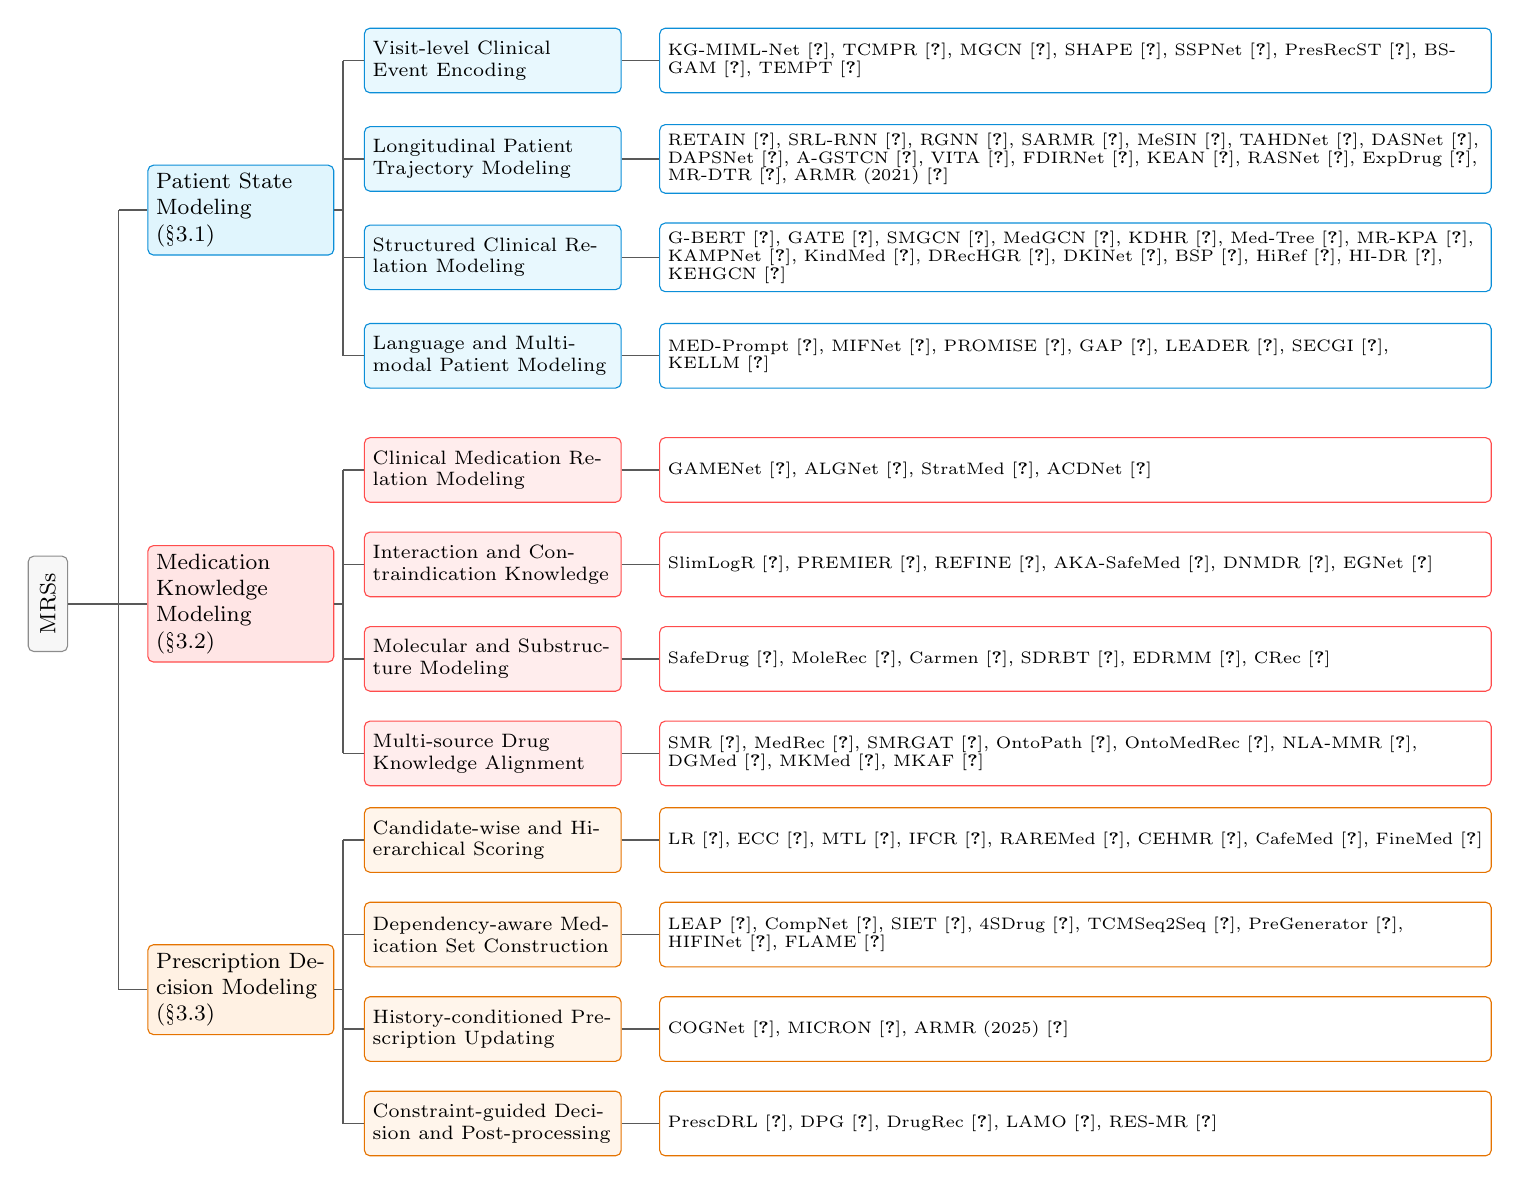
\begin{tikzpicture}[
    font=\footnotesize,
    edge/.style={draw=black!65,line width=0.5pt},
    root/.style={
        draw=black!45,fill=black!3,rounded corners=2pt,align=center,
        text width=1.0cm,minimum height=0.50cm,inner sep=3pt
    },
    stageBlue/.style={
        draw=cyan!75!blue,fill=cyan!12,rounded corners=2pt,align=left,
        text width=2.15cm,minimum height=0.92cm,inner sep=3pt
    },
    catBlue/.style={
        draw=cyan!75!blue,fill=cyan!9,rounded corners=2pt,align=left,
        text width=3.05cm,minimum height=0.82cm,inner sep=3pt,
        font=\fontsize{7.0}{7.8}\selectfont
    },
    listBlue/.style={
        draw=cyan!75!blue,fill=white,rounded corners=2pt,align=left,
        text width=10.35cm,minimum height=0.82cm,inner sep=3pt,
        font=\fontsize{5.6}{6.4}\selectfont
    },
    stageRed/.style={
        draw=red!70,fill=red!10,rounded corners=2pt,align=left,
        text width=2.15cm,minimum height=0.92cm,inner sep=3pt
    },
    catRed/.style={
        draw=red!70,fill=red!7,rounded corners=2pt,align=left,
        text width=3.05cm,minimum height=0.82cm,inner sep=3pt,
        font=\fontsize{7.0}{7.8}\selectfont
    },
    listRed/.style={
        draw=red!70,fill=white,rounded corners=2pt,align=left,
        text width=10.35cm,minimum height=0.82cm,inner sep=3pt,
        font=\fontsize{5.6}{6.4}\selectfont
    },
    stageOrange/.style={
        draw=orange!90!black,fill=orange!11,rounded corners=2pt,align=left,
        text width=2.15cm,minimum height=0.92cm,inner sep=3pt
    },
    catOrange/.style={
        draw=orange!90!black,fill=orange!8,rounded corners=2pt,align=left,
        text width=3.05cm,minimum height=0.82cm,inner sep=3pt,
        font=\fontsize{7.0}{7.8}\selectfont
    },
    listOrange/.style={
        draw=orange!90!black,fill=white,rounded corners=2pt,align=left,
        text width=10.35cm,minimum height=0.82cm,inner sep=3pt,
        font=\fontsize{5.6}{6.4}\selectfont
    }
]

\node[root, rotate=90] (root) at (0,0.20) {MRSs};

\node[stageBlue] (patient) at (2.45,5.20)
{Patient State\\Modeling\\(\S3.1)};
\node[stageRed] (medication) at (2.45,0.20)
{Medication Knowledge Modeling\\(\S3.2)};
\node[stageOrange] (decision) at (2.45,-4.70)
{Prescription Decision Modeling\\(\S3.3)};

\node[catBlue] (p1) at (5.65,7.10)
{Visit-level Clinical Event Encoding};
\node[listBlue] (p1List) at (13.05,7.10)
{KG-MIML-Net~\cite{shangKnowledgeGuidedMultiinstance2018b}, TCMPR~\cite{dongTCMPRTCMPrescription2021}, MGCN~\cite{zhaoTCMHerbalPrescription2022b}, SHAPE~\cite{liu2023shape}, SSPNet~\cite{zhang2025_sspnet}, PresRecST~\cite{dongPresRecSTNovelHerbal2024b}, BSGAM~\cite{tangUtilizingSemanticallyEnhanced2025}, TEMPT~\cite{liu2025tempt}};

\node[catBlue] (p2) at (5.65,5.85)
{Longitudinal Patient Trajectory Modeling};
\node[listBlue] (p2List) at (13.05,5.85)
{RETAIN~\cite{choi2016retain}, SRL-RNN~\cite{wang2018srlrnn}, RGNN~\cite{liuHybridMethodRecurrent2020b}, SARMR~\cite{wangSelfSupervisedAdversarialDistribution2021}, MeSIN~\cite{an2021mesin}, TAHDNet~\cite{su2022tahdnet}, DASNet~\cite{anPredictionTreatmentMedicines2022a}, DAPSNet~\cite{wuDualAttentionPatient2023a}, A-GSTCN~\cite{yueAGSTCNAugmentedGraph2023a}, VITA~\cite{kim2024vita}, FDIRNet~\cite{liuSafeDrugRecommendation2024c}, KEAN~\cite{weiKnowledgeEnhancedAttention2024b}, RASNet~\cite{zhu2024rasnet}, ExpDrug~\cite{luExpDrugExplainableDrug2025b}, MR-DTR~\cite{li2025mrdtr}, ARMR (2021)~\cite{wang2021adversarially}};

\node[catBlue] (p3) at (5.65,4.60)
{Structured Clinical Relation Modeling};
\node[listBlue] (p3List) at (13.05,4.60)
{G-BERT~\cite{shang2019gbert}, GATE~\cite{suGATEGraphAttentionAugmented2020}, SMGCN~\cite{jinSyndromeawareHerbRecommendation2020e}, MedGCN~\cite{mao2022medgcn}, KDHR~\cite{yangMultilayerInformationFusion2022}, Med-Tree~\cite{wang2022medtree}, MR-KPA~\cite{lin2022mrkpa}, KAMPNet~\cite{anKAMPNetMultisourceMedical2023b}, KindMed~\cite{mulyadi2023knowledge}, DRecHGR~\cite{zhang2024drechgr}, DKINet~\cite{liuDKINetMedicationRecommendation2024d}, BSP~\cite{zhaoSequentialPatternsRethinking2025d}, HiRef~\cite{chok2025hiref}, HI-DR~\cite{kimHIDRExploitingHealth2025}, KEHGCN~\cite{zhangKnowledgeEnhancedExplainableHypergraph2026}};

\node[catBlue] (p4) at (5.65,3.35)
{Language and Multimodal Patient Modeling};
\node[listBlue] (p4List) at (13.05,3.35)
{MED-Prompt~\cite{ahmed2024medprompt}, MIFNet~\cite{huoMIFNetMultimodalInteractive2024a}, PROMISE~\cite{wu2024promise}, GAP~\cite{zhongGAPGraphAssistedPrompts2025c}, LEADER~\cite{liu2024leader}, SECGI~\cite{yangSECGIMedicationRecommendation2025}, KELLM~\cite{xu2025kellm}};

\node[catRed] (m1) at (5.65,1.90)
{Clinical Medication Relation Modeling};
\node[listRed] (m1List) at (13.05,1.90)
{GAMENet~\cite{shang2019gamenet}, ALGNet~\cite{nguyenALGNetAttentionLight2023c}, StratMed~\cite{liStratMedRelevanceStratification2024a}, ACDNet~\cite{miACDNetAttentionguidedCollaborative2024b}};

\node[catRed] (m2) at (5.65,0.70)
{Interaction and Contraindication Knowledge};
\node[listRed] (m2List) at (13.05,0.70)
{SlimLogR~\cite{chiang2018drug}, PREMIER~\cite{bhoi2021premier}, REFINE~\cite{bhoi2023refine}, AKA-SafeMed~\cite{yuAKASafeMedSafeMedication2024c}, DNMDR~\cite{liuDNMDRDynamicNetworks2025c}, EGNet~\cite{nguyenEGNetExplainableGraph2025b}};

\node[catRed] (m3) at (5.65,-0.50)
{Molecular and Substructure Modeling};
\node[listRed] (m3List) at (13.05,-0.50)
{SafeDrug~\cite{yang2021safedrug}, MoleRec~\cite{yang2023molerec}, Carmen~\cite{chen2023carmen}, SDRBT~\cite{yangPatientDeepSpatiotemporal2025c}, EDRMM~\cite{liuEDRMMEnhancingDrug2025b}, CRec~\cite{zhangRevisitingDrugRecommendation2025c}};

\node[catRed] (m4) at (5.65,-1.70)
{Multi-source Drug Knowledge Alignment};
\node[listRed] (m4List) at (13.05,-1.70)
{SMR~\cite{gong2021smr}, MedRec~\cite{zhang2023medrec}, SMRGAT~\cite{yangSMRGATTraditionalChinese2023b}, OntoPath~\cite{yao2023ontopath}, OntoMedRec~\cite{tan2024ontomedrec}, NLA-MMR~\cite{tan2024nlamr}, DGMed~\cite{liang2024dual}, MKMed~\cite{li2025bucket}, MKAF~\cite{zhouMultisourceMedicalKnowledge2025b}};

\node[catOrange] (r1) at (5.65,-2.80)
{Candidate-wise and Hierarchical Scoring};
\node[listOrange] (r1List) at (13.05,-2.80)
{LR~\cite{luaces2012binary}, ECC~\cite{read2011classifier}, MTL~\cite{xiaLearningDoctorsMedicine2018b}, IFCR~\cite{chenEpilepsyDrugRecommendation2018b}, RAREMed~\cite{zhao2024raremed}, CEHMR~\cite{wang2023cehmr}, CafeMed~\cite{ren2025cafemed}, FineMed~\cite{li2026medication}};

\node[catOrange] (r2) at (5.65,-4.00)
{Dependency-aware Medication Set Construction};
\node[listOrange] (r2List) at (13.05,-4.00)
{LEAP~\cite{zhang2017leap}, CompNet~\cite{wang2019compnet}, SIET~\cite{wangSafeMedicineRecommendation2022b}, 4SDrug~\cite{tan2022_4sdrug}, TCMSeq2Seq~\cite{li2018tcmseq2seq}, PreGenerator~\cite{zhao2023pregenerator}, HIFINet~\cite{zhengHIFINetExaminationDiagnosisTreatmentHierarchical2024a}, FLAME~\cite{fan2026fine}};

\node[catOrange] (r3) at (5.65,-5.20)
{History-conditioned Prescription Updating};
\node[listOrange] (r3List) at (13.05,-5.20)
{COGNet~\cite{wu2022cognet}, MICRON~\cite{yang2021micron}, ARMR (2025)~\cite{wu2025armr}};

\node[catOrange] (r4) at (5.65,-6.40)
{Constraint-guided Decision and Post-processing};
\node[listOrange] (r4List) at (13.05,-6.40)
{PrescDRL~\cite{yang2024prescdrl}, DPG~\cite{zheng2023dpg}, DrugRec~\cite{sun2022debiased}, LAMO~\cite{zhao2025lamo}, RES-MR~\cite{RESMR}};

\draw[edge] (root.south) -- (0.90,0.20);
\draw[edge] (0.90,5.20) -- (0.90,-4.70);
\draw[edge] (0.90,5.20) -- (patient.west);
\draw[edge] (0.90,0.20) -- (medication.west);
\draw[edge] (0.90,-4.70) -- (decision.west);

\draw[edge] (patient.east) -- (3.75,5.20);
\draw[edge] (3.75,7.10) -- (3.75,3.35);
\draw[edge] (3.75,7.10) -- (p1.west);
\draw[edge] (3.75,5.85) -- (p2.west);
\draw[edge] (3.75,4.60) -- (p3.west);
\draw[edge] (3.75,3.35) -- (p4.west);

\draw[edge] (medication.east) -- (3.75,0.20);
\draw[edge] (3.75,1.90) -- (3.75,-1.70);
\draw[edge] (3.75,1.90) -- (m1.west);
\draw[edge] (3.75,0.70) -- (m2.west);
\draw[edge] (3.75,-0.50) -- (m3.west);
\draw[edge] (3.75,-1.70) -- (m4.west);

\draw[edge] (decision.east) -- (3.75,-4.70);
\draw[edge] (3.75,-2.80) -- (3.75,-6.40);
\draw[edge] (3.75,-2.80) -- (r1.west);
\draw[edge] (3.75,-4.00) -- (r2.west);
\draw[edge] (3.75,-5.20) -- (r3.west);
\draw[edge] (3.75,-6.40) -- (r4.west);

\draw[edge] (p1.east) -- (p1List.west);
\draw[edge] (p2.east) -- (p2List.west);
\draw[edge] (p3.east) -- (p3List.west);
\draw[edge] (p4.east) -- (p4List.west);
\draw[edge] (m1.east) -- (m1List.west);
\draw[edge] (m2.east) -- (m2List.west);
\draw[edge] (m3.east) -- (m3List.west);
\draw[edge] (m4.east) -- (m4List.west);
\draw[edge] (r1.east) -- (r1List.west);
\draw[edge] (r2.east) -- (r2List.west);
\draw[edge] (r3.east) -- (r3List.west);
\draw[edge] (r4.east) -- (r4List.west);

\end{tikzpicture}
\end{adjustbox}
\caption{A component-oriented taxonomy of medication recommendation systems. Each method is shown once according to the component targeted by its principal methodological contribution. Patient state modeling organizes methods by the clinical evidence used to characterize a patient; medication knowledge modeling distinguishes the information used to represent candidate drugs; and prescription decision modeling groups the mechanisms that transform these representations into a medication set. Secondary properties, such as safety control or language-model assistance, are discussed in the corresponding text. Publication years distinguish the two unrelated models both abbreviated as ARMR.}
\label{fig:medication_taxonomy}
\end{figure*}

Medication recommendation systems combine heterogeneous patient evidence, medication knowledge, and decision mechanisms within integrated architectures. A taxonomy based on neural architectures is therefore unstable: graph networks, attention, and language models can operate on different objects and serve different roles in the recommendation process. We instead organize existing systems according to the component targeted by their principal methodological contribution. As shown in Fig.~\ref{fig:medication_taxonomy}, the taxonomy contains three modeling stages: patient state modeling, medication knowledge modeling, and prescription decision modeling. The taxonomy centers on EHR-based methods; non-EHR methods are included only when their modeling mechanisms are relevant to the EHR-based recommendation pipeline.

Each method is assigned one primary position in the figure to keep the taxonomy interpretable and space-efficient. The assignment follows the representation produced by the main technical module. A graph that produces a patient or visit embedding belongs to patient state modeling, whereas a graph that primarily produces drug embeddings belongs to medication knowledge modeling. Historical visits used to encode health trajectories are separated from mechanisms that explicitly copy, add, or remove historical medications. Similarly, DDI information encoded as drug knowledge is distinguished from DDI penalties, logical constraints, or filters that act on the final prescription. Language models are placed according to whether they encode patient evidence, medication descriptions, or the prescription decision itself, rather than being treated as a standalone architecture category.

\subsection{Patient State Modeling}

Patient state modeling converts the clinical evidence available before prescription into a representation of the patient's current therapeutic needs. The evidence may describe heterogeneous events within the target visit, a longitudinal sequence of prior encounters, explicit relations among clinical entities, or narrative information not preserved by discrete codes. We accordingly distinguish visit-level clinical event encoding, longitudinal patient trajectory modeling, structured clinical relation modeling, and language and multimodal patient modeling.

\subsubsection{Visit-level Clinical Event Encoding}

Visit-level clinical event encoding summarizes heterogeneous, unordered observations within a single encounter into a fixed-dimensional representation. The main challenge is to preserve clinically relevant structure despite differences in event type, importance, cardinality, and institutional recording practices. We group existing methods into four categories: \textit{multi-instance event aggregation} handles variable event counts, \textit{attention-based event encoding} weights their relevance, \textit{set-based visit encoding} models order-invariant interactions, and \textit{cross-center visit adaptation} transfers representations across clinical environments.


\textit{Multi-instance Event Aggregation.} Multi-instance methods treat the clinical concepts observed in a visit as multiple evidence instances. They first embed each instance and then aggregate the instance-level representations to describe the complete encounter. A representative method is KG-MIML-Net~\cite{shangKnowledgeGuidedMultiinstance2018b}, which combines multi-instance learning with medical knowledge to model symptom interactions and construct a prescription-oriented visit representation. This design is suitable for visits containing variable numbers of symptoms, although its aggregation quality depends on whether the available knowledge captures the relevant clinical relations.

\textit{Attention-based Event Encoding.} Attention-based methods learn different importance weights for the events within a visit. Instead of assuming that every diagnosis or procedure contributes equally, they emphasize events that are more informative for the target prescription. SHAPE~\cite{liu2023shape}, for example, learns sample-adaptive hierarchical attention to capture both event-level importance and higher-level clinical patterns. Attention improves selective aggregation, but the learned weights should be interpreted as model relevance rather than direct clinical causality.

\textit{Set-based Visit Encoding.} Set-based methods explicitly preserve the unordered nature of clinical events. They use permutation-invariant or permutation-equivariant operations to model dependencies among diagnoses and procedures without introducing an artificial sequence. A representative method is SSPNet~\cite{zhang2025_sspnet}, which employs set attention blocks to encode diagnosis and procedure sets and then fuses their representations for medication prediction. Compared with simple pooling, this formulation captures richer intra-visit interactions, but it also requires sufficient data to learn reliable high-order dependencies.

\textit{Cross-center Visit Adaptation.} Adaptation methods are used when encounter distributions vary across hospitals or clinical centers. They pretrain a transferable visit encoder and introduce a small number of adaptive parameters for the target domain. A representative method is TEMPT~\cite{liu2025tempt}, which combines contrastive pretraining with learned prompts to adapt structured EHR representations across centers. These prompts are model parameters for domain adaptation rather than text instructions or LLM inputs. Visit-level methods provide an informative snapshot of the current condition, but longitudinal modeling is still required when earlier encounters affect the present decision.

Taken together, visit-level methods share the goal of converting heterogeneous events within one encounter into a coherent clinical state, but they address different properties of the input. Multi-instance aggregation handles variable event cardinality, attention identifies events that are more relevant to prescribing, set encoders preserve order invariance, and adaptation methods improve transfer across clinical centers. The appropriate design therefore depends on the structure and source of the current-visit evidence; when treatment decisions depend strongly on earlier encounters, visit-level encoding must be complemented by longitudinal modeling.

\subsubsection{Longitudinal Patient Trajectory Modeling}

Longitudinal patient trajectory modeling captures health-state evolution across visits using historical diagnoses, procedures, and medications. Its central challenge is to retain clinically relevant signals while accounting for outdated records, long-range dependencies, and irregular intervals. We group existing methods into four categories: \textit{recurrent trajectory encoding} sequentially compresses visits, \textit{selective history modeling} retrieves relevant encounters, \textit{long-range trajectory modeling} captures distant dependencies, and \textit{time-aware dynamics modeling} represents visit intervals or treatment stages.

\textit{Recurrent Trajectory Encoding.} Recurrent methods sequentially encode visits and update a hidden state with an RNN, GRU, or LSTM. The hidden state summarizes previous encounters and provides historical context for the current prescription. A representative method is RETAIN~\cite{choi2016retain}, which processes visits in reverse temporal order and with visit- and code-level attention. Its principal modeling target is the longitudinal trajectory, even though attention is used inside the encoder; RETAIN should therefore be placed in this category rather than under intra-visit modeling. Recurrent encoding is efficient for moderate histories, but distant information can be weakened through repeated state updates.

\textit{Selective History Modeling.} Selective-history methods retrieve or weight only the visits that are relevant to the current encounter. They are designed to reduce interference from unrelated diseases, resolved episodes, or obsolete treatments. A representative method is VITA~\cite{kim2024vita}, which first selects historical visits according to their relevance to the target visit and then aggregates their information for medication prediction. This mechanism improves the use of heterogeneous histories, although its effectiveness depends on the reliability of the learned relevance scores.

\textit{Long-range Trajectory Modeling.} Long-range methods use attention, temporal graphs, or advanced sequence encoders to model dependencies that span many encounters. Unlike recurrent compression, they allow the current visit to interact more directly with earlier clinical states. A-GSTCN~\cite{yueAGSTCNAugmentedGraph2023a}, for example, combines graph-based clinical relations with temporal convolution to encode structural and longitudinal dependencies jointly. Such methods capture broader context, but their computational cost grows with the history length and the complexity of the temporal structure.

\textit{Time-aware Dynamics Modeling.} Time-aware methods additionally encode the intervals between visits or the stage of a treatment process. They are useful because two identical event sequences can imply different patient states when their time gaps differ substantially. MR-DTR~\cite{li2025mrdtr}, for example, incorporates relative visit intervals and dynamic treatment regimes into the patient representation. These methods infer patient state from history; methods that directly copy, add, or remove historical medications are discussed later as prescription-updating mechanisms.

Longitudinal methods differ primarily in how they access and retain historical information. Recurrent encoders compress the complete trajectory, selective methods suppress irrelevant visits, long-range architectures expose distant encounters more directly, and time-aware models distinguish histories with different temporal spacing. These choices trade computational efficiency against historical coverage and temporal specificity, while all depend on preventing obsolete or unrelated records from dominating the current state. Importantly, this category uses history to represent the patient rather than to directly reuse or modify earlier prescriptions.

\subsubsection{Structured Clinical Relation Modeling}

Structured clinical relation modeling represents connections among clinical concepts using medical ontologies, EHR-derived co-occurrences, or multi-event associations. The central choice is whether to model predefined hierarchies, pairwise links, or higher-order interactions. Accordingly, we distinguish (1) \textit{ontology-enhanced representation}, which propagates information through medical hierarchies; (2) \textit{graph-based patient representation}, which learns pairwise clinical relations; and (3) \textit{hypergraph and high-order representation}, which captures multi-entity interactions.

\textit{Ontology-enhanced Representation.} Ontology-enhanced methods use parent--child and ancestor--descendant relations in coding systems to regularize clinical concept embeddings. Related codes can share information through the hierarchy, which is useful when individual concepts are sparsely observed. G-BERT~\cite{shang2019gbert}, for example, combines graph-based pretraining over medical ontologies with visit-level sequence modeling. Ontological propagation improves semantic consistency, but a fixed hierarchy may not capture patient-specific relations between concurrent conditions.

\textit{Graph-based Patient Representation.} Graph-based methods construct nodes for clinical entities and edges for their observed or knowledge-derived relations. Graph neural networks then propagate information across related diagnoses, procedures, symptoms, and visits to produce the patient representation. A representative method is GATE~\cite{suGATEGraphAttentionAugmented2020}, which applies graph attention to clinical-event relations and combines the resulting structure-aware representation with temporal information. Graph construction is flexible, although data-derived edges may reflect local documentation and co-occurrence biases.

\textit{Hypergraph and High-order Representation.} Hypergraph methods use one hyperedge to connect several entities and thereby represent interactions that cannot be decomposed into independent pairs. A hyperedge may correspond to a complete visit, a clinical pattern, or a group of mutually related concepts. A representative method is KEHGCN~\cite{zhangKnowledgeEnhancedExplainableHypergraph2026}, which constructs hierarchical hypergraphs at visit and patient levels and augments them with external knowledge paths. High-order modeling preserves richer context, but it introduces additional computational cost and depends on how clinically meaningful hyperedges are constructed.

Structured relation models form a progression from fixed ontology hierarchies to data-dependent pairwise graphs and high-order hypergraphs. Increasing relational flexibility allows the encoder to capture more patient-specific and multi-entity interactions, but it also makes the representation more sensitive to how nodes, edges, and hyperedges are defined. Consequently, model choice should follow the semantics and reliability of the available relations rather than assume that a more complex graph structure is necessarily more informative.

\subsubsection{Language and Multimodal Patient Modeling}

Language and multimodal patient modeling recovers clinical context, such as symptom severity, assessments, negation, and allergies, that structured codes may omit. The central challenge is to align this semantic information with structured EHR evidence. We distinguish three categories: (1) \textit{pretrained language model encoding} derives patient representations from clinical text, (2) \textit{multimodal text--code fusion} integrates narrative and structured evidence, and (3) \textit{LLM-assisted patient semantics} uses LLMs to extract, organize, or reason over patient information.

\textit{Pretrained Language Model Encoding.} Pretrained-language-model methods convert clinical notes into contextual token or document representations and use them for medication prediction. Their basic use is to retain linguistic details that disappear when a record is reduced to diagnosis and procedure codes. A representative method is MED-Prompt~\cite{ahmed2024medprompt}, which reformulates clinical information as prompt-guided inputs and applies BERT-family medical language models to predict medications. These encoders depend on the quality and availability of notes and must avoid text fields that directly reveal the target prescription.

\textit{Multimodal Text--Code Fusion.} Multimodal methods separately encode structured EHR codes and unstructured text before learning interactions between the two modalities. The structured branch captures standardized clinical events, while the text branch supplies contextual semantics. MIFNet~\cite{huoMIFNetMultimodalInteractive2024a}, for example, learns temporal code representations and clinical-text representations and then performs cross-modal interaction and fusion. Multimodal fusion can compensate for missing evidence in either source, but it is sensitive to modality imbalance and unavailable notes.

\textit{LLM-assisted Patient Semantics.} LLM-assisted methods use large language models to extract, transfer, or reason over semantic patient information. A representative method is GAP~\cite{zhongGAPGraphAssistedPrompts2025c}, which constructs a patient-centric graph from medical dialogue and injects the graph into prompts to ground the medication recommendation. This category requires language-derived patient evidence to be part of the main representation process. In contrast, StratMed uses structured diagnosis, procedure, and medication codes without an LLM and is therefore placed under clinical medication relation modeling rather than LLM-derived patient representation.

Language-based methods recover symptom descriptions, assessments, and other contextual evidence that is lost when an encounter is represented only by discrete codes. Pretrained language encoders focus on narrative representation, multimodal methods align narrative and structured evidence, and LLM-assisted methods further organize or reason over patient semantics. Their advantage therefore comes from additional clinical information rather than model scale alone. In practice, this advantage depends on note availability, reliable cross-modal alignment, and controls for target leakage, privacy exposure, and unsupported language-model outputs.

\subsection{Medication Knowledge Modeling}

Medication knowledge modeling determines how candidate drugs are represented before the final prescription is produced. Medication identities alone provide little information about therapeutic similarity, unsafe interactions, chemical properties, or clinical indications. Existing methods therefore learn from clinical medication relations, interaction and contraindication knowledge, molecular structures, or multiple aligned knowledge sources.

\subsubsection{Clinical Medication Relation Modeling}

Clinical medication relation modeling represents candidate drugs through their observed relationships with other medications and patient conditions. We distinguish three evidence scopes: (1) \textit{co-prescription relation modeling} learns population-level drug combinations from EHRs, (2) \textit{patient-conditioned relation modeling} links candidates to the current patient's diagnoses and procedures, and (3) \textit{history--candidate relation modeling} uses prior treatments to assess current candidates.

\textit{Co-prescription Relation Modeling.} Co-prescription methods construct a medication graph in which edges represent drugs that frequently appear together in historical prescriptions. Graph propagation then produces medication embeddings that encode population-level combination patterns. A representative method is GAMENet~\cite{shang2019gamenet}, which builds an EHR medication graph and stores its graph-convolved representations in an external memory for matching with the current patient state. Co-prescription knowledge provides useful empirical priors, but it may reproduce institution-specific habits and cannot by itself establish therapeutic compatibility.

\textit{Patient-conditioned Relation Modeling.} Patient-conditioned methods model the relevance between candidate drugs and the diagnoses or procedures of a specific patient. They are used to suppress weak or noisy biomedical-entity relations and emphasize evidence directly related to the current clinical state. A representative method is StratMed~\cite{liStratMedRelevanceStratification2024a}, which stratifies relations among structured diagnosis, procedure, and medication codes and constructs relevance-driven graphs to alleviate sparse observations. StratMed does not use an LLM; its core contribution is relation stratification over structured biomedical entities.

\textit{History--candidate Relation Modeling.} These methods measure how historical medication information relates to each current candidate. They are useful when a previously prescribed drug or a clinically similar medication provides evidence for current treatment. A representative method is ACDNet~\cite{miACDNetAttentionguidedCollaborative2024b}, which combines historical medication representations with candidate-specific similarity to support collaborative medication prediction. Such relations improve candidate personalization, but inappropriate historical prescriptions can introduce biased evidence.

Clinical medication relation methods connect candidate drugs to progressively more specific evidence. Co-prescription graphs provide population-level combination priors, patient-conditioned relations emphasize diagnoses and procedures relevant to an individual, and history--candidate relations incorporate prior treatment experience. Together, these relations bridge patient evidence and medication representations, but they remain observational signals that may reproduce institutional practice patterns or historical prescribing errors. They should therefore complement, rather than substitute for, molecular and interaction knowledge.

\subsubsection{Interaction and Contraindication Knowledge}

Interaction and contraindication knowledge modeling encodes safety relations among candidate drugs before prescription selection. We distinguish (1) \textit{binary DDI knowledge modeling}, which represents known adverse pairs; (2) \textit{severity-aware interaction modeling}, which differentiates clinical risk levels; and (3) \textit{multi-view safety knowledge modeling}, which combines DDI information with co-prescription or molecular evidence. These methods make drug representations safety-aware, whereas penalties, rules, and filters applied to predicted prescriptions belong to constraint-guided decision modeling.

\textit{Binary DDI Knowledge Modeling.} Binary DDI methods construct a graph whose edges indicate known adverse interactions. The graph is encoded together with EHR or co-prescription information so that candidate representations contain both therapeutic and safety signals. PREMIER~\cite{bhoi2021premier}, for example, jointly uses patient-specific clinical evidence, medication co-occurrence, and DDI relations to support safe recommendation. Binary graphs are straightforward to integrate, but they reduce heterogeneous interaction mechanisms and severities to a single edge type.

\textit{Severity-aware Interaction Modeling.} Severity-aware methods distinguish interactions by their clinical risk instead of treating every DDI equally. This information is used to learn medication relations that reflect the relative consequences of different combinations. A representative method is REFINE~\cite{bhoi2023refine}, which incorporates fine-grained DDI severity and balances recommendation accuracy against different levels of interaction risk. Severity modeling provides more informative safety guidance, although its coverage depends on the completeness and consistency of external annotations.

\textit{Multi-view Safety Knowledge Modeling.} Multi-view methods combine DDI relations with complementary views such as co-prescription patterns, molecular features, or therapeutic associations. They are used to avoid representing drug safety from a single incomplete graph. A representative method is DNMDR~\cite{liuDNMDRDynamicNetworks2025c}, which learns dynamic multi-view drug representations from clinical co-occurrence, adverse interaction, and molecular information. Multi-view representations are more comprehensive, but inaccurate alignment between sources can propagate noise into the drug embeddings.

Interaction modeling becomes progressively more informative as methods move from binary DDI indicators to severity-aware relations and multi-view safety knowledge. This added granularity can distinguish different levels and sources of risk, but it also increases dependence on the coverage, consistency, and alignment of external databases. Moreover, these methods make candidate representations safety-aware before prediction; they do not guarantee that the final medication set obeys a desired risk threshold, which requires decision-level constraints or post-processing.

\subsubsection{Molecular and Substructure Modeling}

Molecular and substructure modeling uses chemical structures to capture drug properties not reliably inferred from identifiers or prescribing statistics. Because global embeddings may obscure condition-relevant components, the central choices are structural granularity and patient conditioning. We distinguish four categories: (1) \textit{whole-molecule graph encoding} summarizes the complete molecular graph, (2) \textit{substructure-aware representation} models local fragments, (3) \textit{context-aware molecular modeling} conditions chemical features on patient evidence, and (4) \textit{causal substructure modeling} separates clinically relevant components from dataset-specific correlations.

\textit{Whole-molecule Graph Encoding.} Whole-molecule methods apply a graph neural network to the complete chemical structure and pool atom-level features into a drug embedding. The embedding can then be matched with the patient representation or combined with DDI knowledge. A representative method is SafeDrug~\cite{yang2021safedrug}, which employs global and local molecular graph encoders and uses the resulting representations for condition-aware medication recommendation. Whole-graph encoding provides a unified chemical view, but global pooling may obscure the local fragments responsible for specific therapeutic effects.

\textit{Substructure-aware Representation.} Substructure methods decompose each molecule into functional fragments and model how individual fragments relate to patient conditions. They are used to provide more fine-grained medication representations and to distinguish drugs with similar global structures. A representative method is MoleRec~\cite{yang2023molerec}, which learns interactions between patient representations and medication substructures before aggregating them for drug prediction. Substructure modeling can improve local interpretability, although learned fragment importance does not necessarily correspond to a verified pharmacological mechanism.

\textit{Context-aware Molecular Modeling.} Context-aware methods modify molecular representations according to the target patient or clinical context. This avoids assuming that structural similarity has the same meaning for every condition. A representative method is Carmen~\cite{chen2023carmen}, which learns context-aware molecular representations to distinguish drugs whose graph structures are similar but whose clinical functions differ. Context conditioning improves specificity, but it requires careful alignment between EHR evidence and molecular features.

\textit{Causal Substructure Modeling.} Causal approaches attempt to separate condition-relevant molecular components from substructures that are predictive only because of dataset-specific correlations. A representative method is CRec~\cite{zhangRevisitingDrugRecommendation2025c}, which uses patient-conditioned representation learning and intervention to reduce reliance on spurious substructures. This direction may improve robustness, but its conclusions depend on the validity of the assumed causal decomposition.

Molecular methods progress from global chemical representations to local fragments, patient-conditioned structures, and causal--spurious decompositions. This progression seeks to make chemical evidence increasingly specific to the therapeutic context and to expose which parts of a molecule influence recommendation. However, finer representations introduce additional assumptions about molecular fragmentation, patient--structure alignment, and causal validity. Molecular evidence is therefore most useful when combined with clinical indications and verified interaction knowledge rather than interpreted in isolation.

\subsubsection{Multi-source Drug Knowledge Alignment}

Multi-source drug knowledge alignment integrates evidence from ontologies, knowledge graphs, text, molecular structures, EHR co-prescriptions, and DDI databases. Because these sources differ in vocabulary, granularity, and coverage, effective integration requires explicit cross-source correspondence beyond feature concatenation. We distinguish (1) \textit{ontology-based alignment} via shared medical hierarchies, (2) \textit{knowledge-graph alignment} via relational paths, and (3) \textit{cross-modal drug alignment} in a coordinated representation space.

\textit{Ontology-based Alignment.} Ontology-based methods use therapeutic, diagnostic, or indication hierarchies to connect medication concepts with related clinical concepts. They pretrain or propagate embeddings over the hierarchy and align them with patient representations. A representative method is OntoMedRec~\cite{tan2024ontomedrec}, which learns model-agnostic ontology encoders and aligns diagnosis and medication concepts for downstream recommendation. Ontologies provide stable semantic structure, but mapping local EHR codes to external concepts can introduce coverage gaps.

\textit{Knowledge-graph Alignment.} Knowledge-graph methods connect medications with diseases, symptoms, treatments, and other biomedical entities. Graph encoders then produce relational drug embeddings that can be matched with the patient's clinical state. A representative method is MedRec~\cite{zhang2023medrec}, which integrates structured medical knowledge to strengthen patient--medication relation learning. Knowledge graphs offer interpretable paths, but missing or noisy edges may bias the resulting representations.

\textit{Cross-modal Drug Alignment.} Cross-modal methods align medication descriptions, molecular structures, interaction graphs, and clinical usage patterns in a shared space. They are particularly useful when no single source describes every candidate drug adequately. A representative method is MKMed~\cite{li2025bucket}, which uses cross-modal alignment and bucket-based learning to retain medications that would otherwise be lost because the source modalities have incomplete intersections. Multi-source alignment broadens medication coverage, although performance remains sensitive to modality imbalance and entity-matching quality.

The three alignment strategies provide complementary forms of medication semantics: ontologies offer stable hierarchies, knowledge graphs encode relational paths, and cross-modal alignment connects textual, structural, interaction, and usage evidence. Their shared goal is to construct drug representations whose coverage exceeds that of any single source. The main bottleneck is not the number of incorporated sources but whether their entities are matched correctly and whether missing, imbalanced, or conflicting modalities are handled without distorting the shared representation.

\subsection{Prescription Decision Modeling}

Prescription decision modeling transforms patient states and medication representations into a final medication set. The decision mechanism determines whether drugs are scored independently, constructed jointly as a set, updated from historical prescriptions, or revised under explicit clinical constraints. We therefore distinguish candidate-wise and hierarchical scoring, dependency-aware medication set construction, history-conditioned prescription updating, and constraint-guided decision and post-processing.

\subsubsection{Candidate-wise and Hierarchical Scoring}

Candidate-wise and hierarchical scoring estimates each drug’s suitability and converts the scores into a multi-label prescription through thresholding or ranking. This scalable formulation differs mainly in how supervision is organized: (1) \textit{independent candidate scoring} learns drug-specific decisions, (2) \textit{hierarchical candidate scoring} transfers supervision through medication taxonomies, and (3) \textit{rare-label candidate scoring} uses pretraining or representation transfer for infrequent diseases and medications.

\textit{Independent Candidate Scoring.} Independent scoring methods formulate medication recommendation as a set of binary prediction problems. Each drug receives a probability based on the patient representation, and drugs above a threshold are selected. A representative method is logistic regression with binary relevance~\cite{luaces2012binary}, which trains one classifier for each medication label. This formulation is computationally efficient and provides a transparent baseline, but it ignores dependencies among drugs and is sensitive to label imbalance and threshold selection.

\textit{Hierarchical Candidate Scoring.} Hierarchical methods exploit medication categories or therapeutic taxonomies before predicting specific drugs. Coarse labels provide shared supervision and constrain fine-grained predictions. A representative method is CEHMR~\cite{wang2023cehmr}, which jointly predicts medication categories and individual medication labels in a hierarchical multi-label framework. Hierarchical supervision improves consistency across related drugs, although the result depends on the quality and granularity of the adopted medication hierarchy.

\textit{Rare-label Candidate Scoring.} Rare-label methods improve scoring for diseases or medications with few training examples. They typically use pretraining, self-supervision, or transfer from common clinical patterns before fine-tuning the prediction head. RAREMed~\cite{zhao2024raremed}, for example, learns code-sequence representations through self-supervised pretraining and then fine-tunes the model for rare-disease medication recommendation. Its main contribution is candidate prediction under scarcity, so it belongs to this category rather than dependency-aware set construction.

Candidate-wise methods retain the same basic parallel-scoring formulation while changing how supervision is organized. Independent classifiers provide scalability and simple optimization, hierarchical objectives share information across related labels, and rare-label methods transfer representation knowledge to sparsely observed candidates. This family is therefore well suited to large medication vocabularies and efficient inference. Its principal limitation is that improving individual scores does not fully capture compatibility, redundancy, or dependence within the selected medication set.

\subsubsection{Dependency-aware Medication Set Construction}

Dependency-aware medication set construction treats a prescription as a coordinated, unordered set and models complementarity, redundancy, and conditional dependence among drugs. Methods differ in when these dependencies enter prediction: (1) \textit{sequential medication generation} conditions on previously generated drugs, (2) \textit{order-free combination prediction} avoids a fixed decoding order, (3) \textit{set-to-set recommendation} directly maps patient-condition sets to medication sets, and (4) \textit{list-wise prescription refinement} evaluates or revises the complete predicted list.

\textit{Sequential Medication Generation.} Sequential methods generate one medication at a time and condition each new decision on the drugs generated previously. This allows the decoder to model conditional dependencies within a prescription. A representative method is LEAP~\cite{zhang2017leap}, which formulates multimorbidity medication recommendation as sequential generation and uses previously generated drugs to guide subsequent choices. Sequential decoding is expressive, but prescriptions are naturally unordered, so an arbitrary generation order may introduce exposure bias.

\textit{Order-free Combination Prediction.} Order-free methods treat medication selection as a set decision and avoid assuming a fixed drug order. They update a prescription state or candidate graph until the combination is complete. A representative method is CompNet~\cite{wang2019compnet}, which formulates medication combination prediction as an order-free decision process with graph-convolutional reinforcement learning. The formulation better matches the set nature of prescriptions, although the action space can become difficult to optimize as the number of candidates grows.

\textit{Set-to-set Recommendation.} Set-to-set methods directly learn a mapping from a set of patient conditions to a set of medications. Their encoders and matching functions are designed to remain invariant to the order of elements on both sides. A representative method is 4SDrug~\cite{tan2022_4sdrug}, which matches symptom sets with drug sets while encouraging small and safe medication combinations. Its main contribution is the construction of an order-free output set, so it is classified here rather than under generic safety control.

\textit{List-wise Prescription Refinement.} List-wise methods evaluate and revise the predicted medication list as a whole. They can remove redundant drugs, introduce missing candidates, or optimize prescription-level feedback after initial generation. A representative method is FLAME~\cite{fan2026fine}, which performs generative alignment and drug-level filtering followed by list-level adjustment. List-wise refinement models global prescription quality, but it requires reliable feedback for evaluating complete medication sets.

Dependency-aware methods differ in when and how interactions among selected drugs are introduced. Sequential generation captures conditional dependence but imposes an order, order-free and set-to-set methods preserve permutation invariance, and list-wise refinement evaluates the prescription after an initial prediction has been formed. These formulations represent prescription-level coherence more directly than independent scoring, but they require more difficult search, optimization, or feedback estimation. The preferred formulation therefore depends on whether output order, global set quality, or post-generation correction is the dominant concern.

\subsubsection{History-conditioned Prescription Updating}

 Physicians often revise existing treatments rather than construct prescriptions from scratch, motivating history-conditioned prescription updating. Historical medication sets can provide evidence about treatment continuity, but they may also contain drugs that have become obsolete after a change in the patient's condition. The central problem is therefore to distinguish medications that should be retained from those that should be discontinued or newly introduced. We organize existing methods into three categories according to the form of prescription revision: (1) \textit{copy-or-predict updating} chooses between reusing historical drugs and generating new ones, (2) \textit{medication change prediction} estimates explicit additions and removals, and (3) \textit{adaptive historical reuse} assigns different roles to long-term and recent treatment histories. This category acts on historical prescriptions as decision objects, whereas longitudinal patient encoders use history primarily to construct the patient state.

\textit{Copy-or-predict Updating.} Copy-based methods reuse medications from previous prescriptions when they remain suitable for the current condition and predict new drugs for unmet needs. A representative method is COGNet~\cite{wu2022cognet}, which introduces a copy-or-predict mechanism to combine reusable historical medications with newly generated candidates. Copying captures treatment continuity and reduces unnecessary reconstruction, but an incorrect reuse decision can propagate obsolete or inappropriate drugs.

\textit{Medication Change Prediction.} Change-prediction methods model the difference between the previous and current prescriptions. Instead of predicting the full output set independently, they estimate which medications should be added or removed according to changes in the patient state. MICRON~\cite{yang2021micron}, for example, represents changes in health conditions and predicts the corresponding medication residual. This formulation is efficient when treatment changes gradually, but may be less suitable after a major clinical event that requires extensive prescription revision.

\textit{Adaptive Historical Reuse.} Adaptive methods distinguish the roles of long-term and recent histories and decide separately which old medications should be reused and which new medications should be introduced. A representative method is ARMR~\cite{wu2025armr}, which models long- and short-term patient histories and adaptively separates reused drugs from new candidates. The additional flexibility better represents chronic treatment and acute changes, although it also requires reliable estimation of when historical evidence remains applicable.

Prescription-updating methods exploit treatment continuity with varying flexibility: copy-or-predict mechanisms reuse suitable historical drugs or generate new ones, residual methods predict additions and removals, and adaptive methods distinguish long-term maintenance from recent changes. This structure can reduce unnecessary reconstruction when therapy evolves gradually, but its assumptions become fragile after abrupt clinical events. Reliable change detection and reuse gating are therefore central to preventing obsolete medications from being propagated.

\subsubsection{Constraint-guided Decision and Post-processing}

Constraint-guided decision and post-processing methods control properties of the final medication set that predictive likelihood alone does not represent adequately, including interaction risk, prescription-level utility, and excessive medication generation. Their defining feature is that the control mechanism acts during prescription construction or revises its output, rather than only enriching the input drug representations. We distinguish three categories according to how the desired behavior is imposed: (1) \textit{policy-based decision optimization} expresses prescription objectives through rewards, (2) \textit{logical constraint-based inference} enforces explicit rules during candidate selection, and (3) \textit{overprescription-aware LLM decision} restricts otherwise open-ended generation through candidate-level or size-controlled outputs. This separation also distinguishes decision-level safety control from DDI knowledge modeling, which encodes safety information before prediction.

\textit{Policy-based Decision Optimization.} Policy-based methods formulate medication selection as a sequence of actions and optimize a reward that combines therapeutic relevance with prescription-level objectives. A representative method is PrescDRL~\cite{yang2024prescdrl}, which learns a drug-oriented prescription policy through deep reinforcement learning. Policy optimization can handle non-differentiable objectives and delayed set-level feedback, but its behavior depends strongly on reward design and the reliability of offline clinical data.

\textit{Logical Constraint-based Inference.} Logical methods first estimate medication suitability and then solve a constrained selection problem. Explicit rules can prevent incompatible pairs or enforce other clinically motivated requirements. A representative method is DrugRec~\cite{sun2022debiased}, which models longitudinal conditions with a causal graph and formulates DDI coordination as a satisfiability problem during inference. Logical post-processing makes the constraint transparent, but overly strict or incomplete rules may remove useful medications.

\textit{Overprescription-aware LLM Decision.} LLM-oriented control methods restrict open-ended medication generation to reduce invalid or unnecessarily long prescriptions. They commonly convert generation into candidate-level classification or apply explicit size and validity constraints. A representative method is LAMO~\cite{zhao2025lamo}, which reformulates LLM-based medication recommendation as medication-level decisions instead of unconstrained list generation. This strategy reduces overprescription risk, although controlling list size must not suppress clinically necessary drugs.

Constraint-guided methods provide different levels of control over the final prescription. Policy optimization expresses preferences through rewards, logical inference enforces explicit rules during selection, and overprescription-aware LLM methods restrict the decision format of otherwise open-ended generation. Unlike safety-aware representation learning, these mechanisms intervene directly in prescription construction or revision. Their effectiveness is nevertheless bounded by the correctness and completeness of the reward, rule set, or output restriction, so constraint satisfaction should not be interpreted as clinical validation.

\section{Benchmark and Comparative Analysis}
\label{sec:benchmark}

\subsection{Benchmark Settings}

We introduce DREAM, a unified medication recommendation benchmark spanning multiple public EHR datasets and medication granularities. DREAM standardizes the task formulation, data preprocessing and medication coding procedures, patient-level data splits, training protocols, and evaluation metrics. By controlling these sources of experimental variation, the benchmark supports fair and reproducible comparisons of representative medication recommendation methods.

\paragraph{Benchmark Availability.}
The implementation of DREAM, including the data preprocessing pipeline, baseline implementations, experimental configurations, and evaluation scripts, is available in an anonymous repository.\footnote{\url{https://github.com/novzyg/DREAM}} Because the source EHR datasets are governed by their respective data-use agreements, the repository does not redistribute raw patient records. Instead, it provides the code and instructions needed by authorized users to construct the processed benchmark datasets and reproduce the evaluation protocol.

\subsubsection{Datasets and Task Setting}

We conduct experiments on three real-world EHR datasets: MIMIC-III, MIMIC-IV, and eICU. These datasets are widely used in medication recommendation and provide longitudinal patient records containing diagnoses, procedures, and medications. We formulate medication recommendation as a next-visit medication prediction task. Each patient is represented as a chronological sequence of admissions, where each admission contains diagnosis, procedure, and medication sets. Given historical admissions and the clinical information of the target admission, the model predicts the medication set for the target admission.

\subsubsection{Data Processing Limitations}

In medication recommendation, raw EHR data are usually converted into chronological visit sequences, where each visit contains diagnoses, procedures, and prescribed medications. Although this preprocessing paradigm has been widely adopted, existing pipelines may introduce inconsistencies that affect model training and evaluation.

First, some studies reduce data sparsity by filtering infrequent diagnosis or procedure codes, such as retaining only the most frequent codes. However, the medications associated with the removed clinical codes are often still kept in the prescription labels. This may weaken the correspondence between the processed patient conditions and the ground-truth medication set, making the recommendation target less clinically consistent.

Second, the construction of DDI information may also introduce safety evaluation bias. Some studies build the DDI matrix from selected side-effect categories or partial interaction records. As a result, the resulting DDI matrix may not fully cover potential adverse drug interactions. Since DDI rate is widely used as a safety metric, an incomplete or biased DDI matrix may lead to unreliable safety evaluation.

\subsubsection{Data Processing and Medication Standardization}
\label{sec:dataset_settings}

To ensure fair comparison across datasets and models, all datasets are processed into a unified admission-level format. Diagnosis, procedure, and medication records are cleaned, aligned by admission, and organized into patient-level longitudinal sequences. For medication standardization, raw drug names are mapped to DrugBank identifiers, and compound medications are decomposed into single-ingredient drugs when possible. DrugBank is further used to obtain ATC codes and molecular structures, while DDInter is used to construct the DDI adjacency matrix for safety evaluation. EHR-based drug co-occurrence matrices and molecular representations are also generated for models that require them.

\subsubsection{Medication Granularity and Safety Knowledge}

To examine the effect of medication granularity, each dataset is processed under three medication-level settings: all-level, ATC-3, and ATC-4. The all-level setting preserves fine-grained standardized drugs, ATC-3 groups drugs into broader therapeutic categories, and ATC-4 provides an intermediate level between fine-grained drug identifiers and coarse therapeutic classes. Dataset statistics under different medication granularities are reported in Table~\ref{tab:dataset_statistics}. Since DDI rate depends on the underlying interaction knowledge, we construct DDI adjacency matrices under each medication granularity level and report the corresponding ground-truth DDI statistics.
LAMO and FLAME are evaluated only at the all level because their text-based fine-grained medication outputs are not directly compatible with the aggregated ATC-3 and ATC-4 label spaces.


\subsubsection{Compared Methods}



We include a broad range of representative medication recommendation methods to support a unified empirical comparison. As summarized in Table~\ref{tab:baseline_models}, these methods cover traditional multi-label learning, longitudinal EHR modeling, graph- and knowledge-enhanced recommendation, safety-aware learning, molecular representation, medication change modeling, set-wise prediction, and PLM/LLM-assisted recommendation. Rather than reintroducing each method in detail, this section focuses on their coverage of major modeling directions, while the methodological details have been reviewed in Section~\ref{sec:taxonomy}. Overall, the selected methods provide a diverse benchmark for comparing representative medication recommendation systems under consistent datasets, medication granularities, and evaluation protocols.


% Fixed-width, left-aligned, and automatically wrapped column
\newcolumntype{L}[1]{>{\RaggedRight\arraybackslash}p{#1}}

\begingroup
\tiny
\setlength{\tabcolsep}{3pt}
\renewcommand{\arraystretch}{1.08}
\setlength{\LTleft}{0pt}
\setlength{\LTright}{0pt}

\begin{longtable}{
    @{}
    L{0.13\textwidth}
    L{0.54\textwidth}
    L{0.27\textwidth}
    @{}
}

\caption{Overview of the evaluated baseline models and their positions in our taxonomy.}
\label{tab:baseline_models}\\

\toprule
\multicolumn{1}{c}{\textbf{Model}} &
\multicolumn{1}{c}{\textbf{Brief Description}} &
\multicolumn{1}{c}{\textbf{Primary Category in Our Taxonomy}} \\
\midrule
\endfirsthead

\multicolumn{3}{c}{
\tablename~\thetable{} -- Continued from previous page
}\\
\toprule
\multicolumn{1}{c}{\textbf{Model}} &
\multicolumn{1}{c}{\textbf{Brief Description}} &
\multicolumn{1}{c}{\textbf{Primary Category in Our Taxonomy}} \\
\midrule
\endhead

\midrule
\multicolumn{3}{r}{Continued on next page}\\
\endfoot

\bottomrule
\endlastfoot

4SDrug~\cite{tan2022_4sdrug} &
Formulates medication recommendation as symptom-set-to-drug-set prediction and directly models the relationships between symptoms and candidate medications. &
Dependency-aware Medication Set Construction \\
\hline

SSPNet~\cite{zhang2025_sspnet} &
Uses permutation-consistent set encoders and decoders to represent clinical information and predict unordered medication sets. &
Visit-level Clinical Event Encoding \\
\hline

PREMIER~\cite{bhoi2021premier} &
Integrates patient-specific clinical information with drug co-occurrence and interaction knowledge to construct personalized patient representations. &
Interaction and Contraindication Knowledge \\
\hline

VITA~\cite{kim2024vita} &
Introduces target-aware history selection to identify historical visits that are most relevant to the current patient state. &
Longitudinal Patient Trajectory Modeling \\
\hline

RAREMed~\cite{zhao2024raremed} &
Improves patient representation and medication prediction under rare-disease and long-tail clinical distributions. &
Candidate-wise and Hierarchical Scoring \\
\hline

MR-DTR~\cite{li2025mrdtr} &
Models relative time intervals and treatment-stage information to construct time-aware longitudinal patient representations. &
Longitudinal Patient Trajectory Modeling \\
\hline

ARMR~\cite{wu2025armr} &
Dynamically models the relationships among the current patient state, historical visits, and previous medication records. &
History-conditioned Prescription Updating \\
\hline

G-BERT~\cite{shang2019gbert} &
Uses medical ontologies and graph-based pretraining to capture hierarchical relationships among clinical concepts. &
Structured Clinical Relation Modeling \\
\hline

DRecHGR~\cite{zhang2024drechgr} &
Employs heterogeneous graph learning to model structural relations among patients, diagnoses, procedures, and medications. &
Structured Clinical Relation Modeling \\
\hline

TEMPT~\cite{liu2025tempt} &
Uses transfer learning and prompt-based modeling to improve patient representations across heterogeneous clinical centers. &
Visit-level Clinical Event Encoding \\
\hline

LEADER~\cite{liu2024leader} &
Transfers semantic knowledge from large language models to a compact recommendation model through feature-level distillation. &
Language and Multimodal Patient Modeling \\
\hline

GAMENet~\cite{shang2019gamenet} &
Constructs graph-augmented memory representations by incorporating medication co-occurrence and DDI relations. &
Clinical Medication Relation Modeling \\
\hline

COGNet~\cite{wu2022cognet} &
Models relationships between historical and candidate medications through a conditional copy-or-predict framework. &
History-conditioned Prescription Updating \\
\hline

REFINE~\cite{bhoi2023refine} &
Incorporates severity-aware drug interactions and fine-grained clinical trends to support safer medication recommendation. &
Interaction and Contraindication Knowledge \\
\hline

Carmen~\cite{chen2023carmen} &
Enhances medication representations by integrating context-aware molecular information with DDI-related knowledge. &
Molecular and Substructure Modeling \\
\hline

SafeDrug~\cite{yang2021safedrug} &
Represents medications through molecular graphs and uses a DDI-controllable objective to reduce unsafe drug combinations. &
Molecular and Substructure Modeling \\
\hline

MoleRec~\cite{yang2023molerec} &
Models relationships between patient health conditions and medication substructures for fine-grained pharmacological representation. &
Molecular and Substructure Modeling \\
\hline

MedRec~\cite{zhang2023medrec} &
Combines historical medication records and patient trajectory information to support personalized medication prediction. &
Multi-source Drug Knowledge Alignment \\
\hline

OntoPath~\cite{yao2023ontopath} &
Integrates ontology paths and treatment-related paths to enrich medication and clinical concept representations. &
Multi-source Drug Knowledge Alignment \\
\hline

LR~\cite{luaces2012binary} &
Uses independent logistic classifiers to estimate the probability of each medication from the input patient features. &
Candidate-wise and Hierarchical Scoring \\
\hline

ECC~\cite{read2011classifier} &
Uses an ensemble of classifier chains to capture conditional dependencies among medication labels. &
Candidate-wise and Hierarchical Scoring \\
\hline

RETAIN~\cite{choi2016retain} &
Uses reverse-time attention over historical visits and medical codes to perform interpretable multi-label prediction. &
Longitudinal Patient Trajectory Modeling \\
\hline

DPG~\cite{zheng2023dpg} &
Treats medication recommendation as policy learning and learns treatment decisions under sequential patient states. &
Constraint-guided Decision and Post-processing \\
\hline

LEAP~\cite{zhang2017leap} &
Generates medications sequentially and explicitly models dependencies among drugs during the decoding process. &
Dependency-aware Medication Set Construction \\
\hline

CompNet~\cite{wang2019compnet} &
Models order-free medication combinations through graph convolutional reinforcement learning. &
Dependency-aware Medication Set Construction \\
\hline

FLAME~\cite{fan2026fine} &
Formulates medication recommendation as list-wise generation and refines the predicted prescription at the medication-set level. &
Dependency-aware Medication Set Construction \\
\hline

MICRON~\cite{yang2021micron} &
Predicts medication additions and removals between consecutive visits instead of reconstructing the complete prescription. &
History-conditioned Prescription Updating \\
\hline

DrugRec~\cite{sun2022debiased} &
Models treatment and medication changes from a causal perspective to reduce hidden recommendation bias. &
Constraint-guided Decision and Post-processing \\
\hline

LAMO~\cite{zhao2025lamo} &
Uses language-assisted modeling to improve medication prediction while considering effectiveness, safety, and prescription size. &
Constraint-guided Decision and Post-processing \\

\end{longtable}

\endgroup

\subsubsection{Training and Evaluation Protocol}

For each dataset and medication granularity level, patients are divided into training, validation, and test sets with a ratio of 66\%/17\%/17\%. All experiments are repeated with five random seeds, and the results are reported as the mean and standard deviation.

All models are trained using Adam for at most 50 epochs. Hyperparameters are selected by grid search according to the validation Jaccard score. Specifically, the learning rate is searched over $\{1\times10^{-4}, 5\times10^{-4}, 1\times10^{-3}, 5\times10^{-3}\}$, the weight decay coefficient over $\{0, 1\times10^{-5}, 1\times10^{-4}, 1\times10^{-3}, 1\times10^{-2}\}$, and the gradient clipping threshold over $\{0.5, 1.0, 2.0, 5.0\}$. Since each sample contains the complete visit sequence of one patient, training is performed at the single-patient level. Early stopping is applied when the validation Jaccard score does not improve for 10 consecutive epochs, and the best checkpoint is used for testing.

We evaluate recommendation accuracy using Jaccard, PRAUC, precision, recall, and F1-score, while DDI rate is used as a proxy for potential medication safety. Therefore, DDI rate is analyzed jointly with recommendation accuracy and prescription size.

% For each dataset and medication granularity level, patients are split into training, validation, and test sets with a ratio of 66\%/17\%/17\% at the patient level. All experiments are repeated with five random seeds, and the final results are reported as the mean and standard deviation.

% All compared models are trained under a unified experimental protocol. We use the Adam optimizer with a learning rate of $1\times10^{-3}$, set the maximum number of training epochs to 50, and apply gradient clipping with a threshold of 0.5. Since each sample corresponds to the full visit sequence of one patient, the effective batch is constructed at the single-patient level. During training, models are evaluated on the validation set after each epoch, and the checkpoint with the best validation Jaccard score is selected for final testing. Early stopping is adopted when the validation Jaccard score does not improve for 10 consecutive epochs.

% We evaluate model performance using both accuracy-oriented and safety-oriented metrics defined in Section~\ref{sec:metrics}. Accuracy-oriented metrics include Jaccard, PRAUC, average precision, average recall, and average F1-score. We also report the average number of recommended medications to assess prescription compactness. For safety evaluation, we use DDI rate, which measures the proportion of known drug-drug interaction pairs among all predicted drug pairs. Since DDI rate is only a proxy for potential medication safety rather than an absolute clinical contraindication criterion, we analyze it jointly with accuracy metrics and the average number of recommended medications.


% \subsubsection{Parameter Settings}
% All compared models are trained under a unified experimental protocol. We use the Adam optimizer with a learning rate of $1\times10^{-3}$. The maximum number of training epochs is set to 50. Gradient clipping is applied with a threshold of 5.0 to stabilize the training process. Since each sample corresponds to the full visit sequence of one patient, the effective batch is constructed at the single-patient level

% During training, the model is evaluated on the validation set after each epoch. The checkpoint with the best validation Jaccard score is selected for final testing. Early stopping is adopted when the validation Jaccard score does not improve for 10 consecutive epochs. This setting helps reduce overfitting while ensuring that the selected checkpoint achieves the best validation performance.

% For testing, we load the checkpoint with the highest validation Jaccard score under each random seed and evaluate it on the corresponding test set. We use both accuracy-oriented and safety-oriented metrics. The accuracy-oriented metrics include Jaccard, PRAUC, average precision, average recall, and average F1-score. We also report the average number of recommended medications to evaluate the compactness of the predicted medication set. For safety evaluation, we use DDI rate, which measures the proportion of drug pairs with known drug-drug interaction edges among all predicted drug pairs.

% It should be noted that DDI rate is used as an evaluation proxy for potential medication safety rather than an absolute measure of clinical contraindication. Therefore, we jointly analyze DDI rate with accuracy metrics and the average number of recommended medications to provide a more comprehensive evaluation of medication recommendation performance.

% \subsubsection{Dataset Settings}
% \label{sec:dataset_settings}


\begin{table*}
\centering
\scriptsize
\caption{Basic statistics of the processed datasets under different medication granularity levels.}
\label{tab:dataset_statistics}
\begin{tabular}{llrrrrrr}
\toprule
\textbf{Dataset} & \textbf{Med. Level} & \textbf{\#Patients} & \textbf{\#Visits} & \textbf{\#Diagnoses} & \textbf{\#Medications} & \textbf{\#Procedures} & \textbf{DDI Rate} \\
\midrule
\multirow{3}{*}{eICU} 
& All-level & 10,568 & 23,080 & 2,575 & 155 & 2,054 & 0.0781 \\
& ATC3      & 10,526 & 22,988 & 2,572 & 75  & 2,052 & 0.5137 \\
& ATC4      & 10,526 & 22,988 & 2,572 & 107 & 2,052 & 0.3071 \\
\midrule
\multirow{3}{*}{MIMIC-III} 
& All-level & 6,360 & 16,976 & 4,672 & 718 & 1,420 & 0.0819 \\
& ATC3      & 6,359 & 16,974 & 4,672 & 148 & 1,420 & 0.5465 \\
& ATC4      & 6,359 & 16,974 & 4,672 & 317 & 1,420 & 0.3279 \\
\midrule
\multirow{3}{*}{MIMIC-IV} 
& All-level & 8,949 & 24,106 & 11,030 & 877 & 4,810 & 0.0589 \\
& ATC3      & 8,946 & 24,100 & 11,029 & 158 & 4,810 & 0.4872 \\
& ATC4      & 8,946 & 24,100 & 11,029 & 348 & 4,810 & 0.2836 \\
\bottomrule
\end{tabular}
\end{table*}


% We formulate medication recommendation as a next-visit medication prediction task. Each patient is represented as a chronological sequence of admissions, where each admission contains diagnosis, procedure, and medication sets. Given the historical admissions and the clinical information of the target admission, the model predicts the medication set for the target admission.

% Experiments are conducted on three real-world EHR datasets: MIMIC-III, MIMIC-IV, and eICU. To ensure fair comparison, all datasets are processed into a unified admission-level format. Diagnosis, procedure, and medication records are cleaned, aligned by admission, and organized into patient-level longitudinal sequences.

% For medication standardization, raw drug names are mapped to DrugBank identifiers, and compound medications are decomposed into single-ingredient drugs when possible. DrugBank is further used to obtain ATC codes and molecular structures, while DDInter is used to construct the DDI adjacency matrix for safety evaluation. EHR-based drug co-occurrence matrices and molecular representations are also generated for models that require them.

% To evaluate the effect of medication granularity, each dataset is processed under three settings: all-level, ATC-3, and ATC-4. The all-level setting preserves fine-grained standardized drugs, ATC-3 reduces label sparsity by grouping drugs into broader therapeutic categories, and ATC-4 provides an intermediate level between the two. Dataset statistics are reported in Table~\ref{tab:dataset_statistics}.

% For each dataset and granularity level, patients are split into training, validation, and test sets with a ratio of 66\%/17\%/17\% at the patient level. All experiments are repeated with five random seeds, and the final results are reported as the mean and standard deviation.






% \subsection{Baseline Models}
% %介绍常用的代表性模型，可以使用一个表格来总结一下各种模型
% To provide a comprehensive comparison, we include a broad range of representative medication recommendation models as baselines. These methods cover traditional multi-label learning, longitudinal EHR modeling, graph-enhanced recommendation, knowledge-aware modeling, molecular-structure-based recommendation, causal modeling, prescription generation, set-wise prediction, and LLM-assisted recommendation. Instead of further categorizing these baselines, we briefly introduce the main innovation of each method as follows.

% \textbf{LR.}
% Logistic Regression (LR) is used as a traditional linear multi-label prediction baseline. It independently estimates the probability of each medication based on the input patient features, providing a simple reference for evaluating the effectiveness of more advanced deep learning models.

% \textbf{ECC.}
% Ensemble Classifier Chains (ECC) is a classical multi-label learning method that models label dependencies through classifier chains. Compared with independent binary classification, ECC considers the correlations among medication labels and serves as a stronger traditional baseline.

% \textbf{RETAIN.}
% RETAIN~\cite{choi2016retain} is an interpretable model for longitudinal EHR prediction. It uses a reverse-time attention mechanism to capture important historical visits and medical codes, making it suitable for modeling patient trajectories while providing visit-level and code-level interpretability.

% \textbf{LEAP.}
% LEAP~\cite{zhang2017leap} is an early medication recommendation model that formulates treatment recommendation as a sequential decision-making problem. It generates medications step by step and explicitly models dependencies among medication labels during the decoding process.

% \textbf{GAMENet.}
% GAMENet~\cite{shang2019gamenet} introduces graph-augmented memory networks for medication recommendation. It combines longitudinal patient records with external knowledge from EHR co-occurrence graphs and DDI graphs, aiming to improve both recommendation accuracy and medication safety.

% \textbf{G-BERT.}
% G-BERT~\cite{shang2019gbert} incorporates medical ontologies into a pre-training framework for medication recommendation. By using hierarchical diagnosis and medication knowledge, it improves medical code representation and alleviates the limitation of insufficient longitudinal visits.

% \textbf{CompNet.}
% CompNet~\cite{wang2019compnet} focuses on medication combination modeling. It considers the order-free nature of medication combinations and models the recommendation process with graph convolutional reinforcement learning, aiming to capture dependencies among drugs in a prescription.

% \textbf{MICRON.}
% MICRON~\cite{yang2021micron} formulates medication recommendation as a medication change prediction problem. Instead of predicting the complete medication set from scratch, it models the addition and removal of medications between consecutive visits, which better reflects clinical prescription adjustment.

% \textbf{SafeDrug.}
% SafeDrug~\cite{yang2021safedrug} introduces drug molecular structures into medication recommendation. It uses molecular graph representations and a DDI-controllable loss to recommend effective medication combinations while reducing the risk of adverse drug-drug interactions.

% \textbf{COGNet.}
% COGNet~\cite{wu2022cognet} proposes a conditional generation framework with a copy-or-predict mechanism. It determines whether each medication should be copied from historical prescriptions or newly predicted according to the current patient state, thereby better utilizing historical medication information.

% \textbf{PREMIER.}
% PREMIER~\cite{bhoi2021premier} is a personalized medication recommendation model that integrates patient-specific information with drug co-occurrence and DDI knowledge. It aims to improve recommendation accuracy while maintaining medication safety through graph-enhanced representation learning.

% \textbf{4SDrug.}
% 4SDrug~\cite{tan2022_4sdrug} formulates medication recommendation as a symptom-based set-to-set prediction task. It emphasizes recommending small and safe drug sets by modeling symptom sets and drug sets directly, while incorporating both knowledge-based and data-driven DDI constraints.

% \textbf{DrugRec.}
% DrugRec~\cite{sun2022debiased} revisits medication recommendation from a causal perspective. It aims to reduce hidden recommendation bias and improve the reliability of drug prediction by modeling causal relationships among patient conditions, treatments, and medication outcomes.

% \textbf{REFINE.}
% REFINE~\cite{bhoi2023refine} models fine-grained longitudinal clinical trends for medication recommendation. It captures medication dosage titration trends and laboratory response trends, and further considers severity-aware drug interactions to support safer medication prediction.

% \textbf{MedRec.}
% MedRec~\cite{zhang2023medrec} is included as a historical-record-based medication recommendation baseline. It utilizes patient historical visits and medication records to support personalized medication prediction, representing memory-based or trajectory-based recommendation methods.

% \textbf{MoleRec.}
% MoleRec~\cite{yang2023molerec} further explores molecular substructure information for medication recommendation. It models the relationship between patient health conditions and drug substructures, enabling fine-grained pharmacological representation and safety-aware recommendation.

% \textbf{Carmen.}
% Carmen~\cite{chen2023carmen} enhances medication representation by incorporating context-aware molecular graph information and DDI-related knowledge. It aims to distinguish medications with subtle structural or functional differences and improve the safety of recommended drug combinations.

% \textbf{OntoPath.}
% OntoPath~\cite{yao2023ontopath} utilizes ontology paths and treatment-related paths to enhance medication recommendation. By exploiting hierarchical medical knowledge and pathway information, it improves the semantic representation of diagnoses, procedures, and medications.

% \textbf{DPG.}
% DPG~\cite{zheng2023dpg} models medication recommendation from a policy learning perspective. It treats treatment recommendation as a dynamic decision-making process and learns medication policies under sequential patient states.

% \textbf{VITA.}
% VITA~\cite{kim2024vita} focuses on selecting useful historical information for the current visit. It introduces target-aware mechanisms to identify relevant past visits and reduce the influence of noisy or irrelevant historical records.

% \textbf{DRecHGR.}
% DRecHGR~\cite{zhang2024drechgr} employs heterogeneous graph representation learning for medication recommendation. It models complex relations among patients, diagnoses, procedures, and medications, thereby capturing richer structural dependencies in EHR data.

% \textbf{RAREMed.}
% RAREMed~\cite{zhao2024raremed} focuses on medication recommendation for rare disease patients. It aims to improve recommendation performance under long-tail disease distributions and reduce the performance gap between common and rare disease groups.

% \textbf{MR-DTR.}
% MR-DTR~\cite{li2025mrdtr} incorporates dynamic treatment regime information into medication recommendation. It models time-aware patient representations and treatment-stage-specific medication decisions by considering relative time intervals and longitudinal treatment trajectories.

% \textbf{TEMPT.}
% TEMPT~\cite{liu2025tempt} addresses multi-center medication recommendation with transfer and prompt-based learning. It is designed to improve generalization across different clinical distributions and reduce the impact of data heterogeneity among hospitals.

% \textbf{ARMR.}
% ARMR~\cite{wu2025armr} proposes an adaptively responsive network for medication recommendation. It dynamically balances historical medication reuse and new medication prediction according to the current patient state and medication history.

% \textbf{SSPNet.}
% SSPNet~\cite{zhang2025_sspnet} formulates medication recommendation as a set prediction problem. It uses permutation-consistent set encoders and decoders to directly predict unordered medication sets, avoiding artificial medication ordering in prescription generation.

% \textbf{LEADER.}
% LEADER~\cite{liu2024leader} explores LLM-assisted medication recommendation through feature-level knowledge distillation. It leverages the semantic understanding ability of large language models and transfers such knowledge to a smaller medication recommendation model for efficient inference.

% \textbf{LAMO.} 
% LAMO~\cite{zhao2025lamo} is an LLM-based medication recommendation model that introduces language-assisted modeling into medication prediction. It leverages textual clinical information and large language models to enhance patient representation and improve medication recommendation performance.

% \textbf{FLAME.}
% FLAME~\cite{fan2026fine} is a generative medication recommendation model based on large language models. It formulates medication recommendation as a list-wise generation process and refines the predicted medication set by considering prescription-level accuracy and medication safety.

% Overall, these baselines provide a comprehensive comparison with different modeling strategies, ranging from traditional multi-label prediction to recent knowledge-enhanced, molecular-aware, causal, set-wise, and LLM-assisted medication recommendation methods.

\begin{table}[p]
\centering


\makebox[\textwidth][c]{%
\rotatebox{90}{%

\begin{minipage}{0.97\textheight}
\centering


\caption{All-level results on MIMIC-III, MIMIC-IV, and eICU datasets.}
\label{tab:all_level_results}

\footnotesize
\setlength{\tabcolsep}{4pt}
\renewcommand{\arraystretch}{1.5}

\resizebox{\linewidth}{!}{%
\begin{tabular}{lcccccccccccc}
\toprule
\rowcolor{headergray}
& \multicolumn{4}{c}{MIMIC-III}
& \multicolumn{4}{c}{MIMIC-IV}
& \multicolumn{4}{c}{eICU} \\

\rowcolor{headergray}
\multicolumn{1}{c}{\multirow{-2}{*}{Method}}
& Jaccard (\%) $\uparrow$ & PRAUC (\%) $\uparrow$ & F1 (\%) $\uparrow$ & DDI (\%) $\downarrow$
& Jaccard (\%) $\uparrow$ & PRAUC (\%) $\uparrow$ & F1 (\%) $\uparrow$ & DDI (\%) $\downarrow$
& Jaccard (\%) $\uparrow$ & PRAUC (\%) $\uparrow$ & F1 (\%) $\uparrow$ & DDI (\%) $\downarrow$ \\
\midrule

\rowcolor{rowgrayA}
LR & $26.09\pm1.47$ & $33.52\pm2.87$ & $39.87\pm2.02$ & $7.34\pm0.23$ & $27.28\pm0.48$ & $43.25\pm0.62$ & $41.50\pm0.57$ & $6.61\pm0.13$ & $14.40\pm0.77$ & $32.07\pm1.12$ & $27.56\pm1.13$ & $6.48\pm0.63$ \\

\rowcolor{rowgrayB}
ECC & $25.64\pm1.62$ & $47.23\pm0.62$ & $39.03\pm2.42$ & $7.28\pm0.23$ & $25.65\pm0.49$ & $51.31\pm0.40$ & $38.93\pm0.62$ & $6.55\pm0.13$ & $11.66\pm1.09$ & $30.26\pm0.26$ & $26.93\pm1.75$ & $6.69\pm0.63$ \\

\rowcolor{rowgrayC}
RETAIN & $27.97\pm0.31$ & $50.85\pm0.30$ & $42.48\pm0.41$ & $7.35\pm0.12$ & $29.96\pm0.29$ & $53.17\pm0.22$ & $45.04\pm0.32$ & $6.49\pm0.28$ & $18.58\pm0.39$ & \third{$45.49\pm0.35$} & $28.15\pm0.56$ & $6.63\pm0.75$ \\

\rowcolor{rowgrayA}
LEAP & $23.76\pm0.33$ & $33.09\pm1.03$ & $37.06\pm0.40$ & $7.16\pm0.50$ & $27.73\pm0.26$ & $35.82\pm1.16$ & $42.31\pm0.33$ & $6.43\pm0.27$ & $10.12\pm0.53$ & $27.10\pm1.88$ & $15.62\pm0.85$ & $6.57\pm1.45$ \\

\rowcolor{rowgrayB}
GAMENet & $21.43\pm0.46$ & $40.59\pm1.55$ & $34.44\pm0.61$ & $7.37\pm0.37$ & $20.99\pm0.51$ & $46.16\pm0.50$ & $33.91\pm0.69$ & $6.39\pm0.09$ & $23.00\pm0.47$ & $42.70\pm0.95$ & $35.03\pm0.60$ & $7.83\pm0.45$ \\

\rowcolor{rowgrayC}
G-BERT & $23.20\pm0.43$ & $47.36\pm0.46$ & $36.43\pm0.54$ & $7.31\pm0.20$ & $24.21\pm0.57$ & $51.04\pm0.38$ & $38.11\pm0.74$ & $6.58\pm0.10$ & $18.35\pm0.36$ & $43.23\pm0.48$ & $28.05\pm0.72$ & \third{$6.45\pm0.67$} \\

\rowcolor{rowgrayA}
CompNet & $17.76\pm1.35$ & $43.00\pm0.33$ & $29.34\pm1.98$ & $7.25\pm1.78$ & $19.95\pm0.71$ & $45.95\pm0.34$ & $32.44\pm0.95$ & $6.52\pm0.78$ & $10.52\pm2.36$ & $38.61\pm0.66$ & $16.57\pm3.89$ & $6.66\pm0.90$ \\

\rowcolor{rowgrayB}
MICRON & $28.89\pm0.25$ & $53.71\pm0.70$ & $43.80\pm0.29$ & $7.19\pm0.13$ & $29.12\pm0.25$ & $56.59\pm0.28$ & $44.23\pm0.30$ & $6.46\pm0.04$ & $23.06\pm0.36$ & $43.30\pm0.44$ & $35.12\pm0.40$ & $6.60\pm0.26$ \\

\rowcolor{rowgrayC}
SafeDrug & $25.64\pm0.41$ & $49.70\pm0.43$ & $39.81\pm0.55$ & \second{$6.91\pm0.06$} & $26.16\pm0.80$ & $53.39\pm0.34$ & $40.59\pm0.99$ & \second{$6.12\pm0.03$} & $20.93\pm0.49$ & $40.96\pm0.38$ & $32.46\pm0.61$ & \second{$6.20\pm0.64$} \\

\rowcolor{rowgrayA}
COGNet & $22.86\pm3.71$ & $52.87\pm0.79$ & $35.59\pm4.92$ & $7.34\pm0.69$ & $26.69\pm0.86$ & $55.76\pm0.59$ & $40.60\pm1.18$ & $6.61\pm1.50$ & $17.81\pm0.94$ & $44.21\pm0.64$ & $26.79\pm1.30$ & $6.48\pm0.49$ \\

\rowcolor{rowgrayB}
PREMIER & $28.36\pm0.46$ & $50.37\pm0.62$ & $43.08\pm0.57$ & $8.29\pm0.06$ & $29.42\pm0.78$ & $54.00\pm0.27$ & $44.49\pm0.93$ & \third{$6.15\pm0.08$} & \third{$24.33\pm0.23$} & $45.36\pm0.54$ & $36.39\pm0.18$ & $7.08\pm0.22$ \\

\rowcolor{rowgrayC}
4SDrug & $29.48\pm0.45$ & $49.77\pm0.79$ & $44.56\pm0.47$ & $6.97\pm0.23$ & $29.62\pm0.42$ & $54.40\pm0.45$ & $44.61\pm0.45$ & $6.49\pm0.14$ & $24.06\pm0.41$ & $43.70\pm0.72$ & $36.24\pm0.42$ & $6.63\pm0.61$ \\

\rowcolor{rowgrayA}
DrugRec & $21.26\pm0.52$ & $35.26\pm0.84$ & $34.41\pm0.63$ & $7.10\pm0.32$ & $28.40\pm0.60$ & $47.93\pm0.72$ & $42.96\pm0.67$ & $6.43\pm0.19$ & $19.43\pm0.52$ & $38.63\pm0.92$ & $28.29\pm0.59$ & $6.57\pm0.59$ \\

\rowcolor{rowgrayB}
REFINE & $29.68\pm0.38$ & $49.35\pm0.90$ & \third{$44.73\pm0.43$} & $8.26\pm0.16$ & $29.77\pm0.43$ & $53.07\pm0.86$ & $44.98\pm0.52$ & $6.24\pm0.12$ & \second{$24.50\pm0.44$} & $45.09\pm0.57$ & \third{$36.91\pm0.48$} & $6.66\pm0.66$ \\

\rowcolor{rowgrayC}
MedRec & $25.92\pm0.72$ & $51.78\pm0.45$ & $39.28\pm0.90$ & \third{$6.93\pm0.27$} & $29.03\pm0.18$ & $55.17\pm0.30$ & $43.49\pm0.25$ & $6.58\pm0.14$ & $12.67\pm0.63$ & $42.06\pm0.50$ & $19.38\pm0.93$ & \third{$6.45\pm0.27$} \\

\rowcolor{rowgrayA}
MoleRec & $28.77\pm0.25$ & $50.19\pm0.50$ & $43.63\pm0.31$ & \best{$6.56\pm0.15$} & $27.99\pm0.25$ & $53.19\pm0.84$ & $42.89\pm0.31$ & \best{$5.77\pm0.10$} & $22.27\pm0.51$ & $42.71\pm0.52$ & $33.93\pm0.67$ & \best{$5.85\pm0.46$} \\

\rowcolor{rowgrayB}
Carmen & $26.75\pm0.27$ & $50.55\pm0.83$ & $41.28\pm0.35$ & $8.08\pm0.15$ & $27.68\pm0.19$ & $52.34\pm0.28$ & $42.50\pm0.22$ & $6.35\pm0.07$ & $22.16\pm0.38$ & $41.72\pm0.72$ & $33.86\pm0.44$ & $6.60\pm0.65$ \\

\rowcolor{rowgrayC}
OntoPath & $24.59\pm0.94$ & $46.29\pm1.41$ & $37.77\pm1.25$ & $7.79\pm0.73$ & $28.54\pm0.78$ & $51.04\pm0.44$ & $42.98\pm0.97$ & $6.40\pm0.37$ & $10.76\pm1.90$ & $39.46\pm0.61$ & $16.87\pm2.97$ & $6.54\pm1.69$ \\

\rowcolor{rowgrayA}
VITA & $26.20\pm3.87$ & $53.08\pm1.00$ & $39.87\pm2.30$ & $7.34\pm0.95$ & $31.00\pm2.13$ & $56.34\pm0.11$ & $46.10\pm2.54$ & $6.61\pm0.08$ & $17.01\pm2.21$ & $44.90\pm0.37$ & $26.26\pm2.50$ & $6.48\pm1.27$ \\

\rowcolor{rowgrayB}
DRecHGR & $27.94\pm0.46$ & $46.59\pm0.78$ & $43.13\pm0.55$ & $7.78\pm0.22$ & $31.81\pm0.38$ & $53.31\pm0.78$ & $47.39\pm0.43$ & $6.55\pm0.10$ & $20.60\pm0.58$ & $41.28\pm0.70$ & $30.47\pm0.63$ & $6.69\pm0.30$ \\

\rowcolor{rowgrayC}
RAREMed & $27.69\pm0.10$ & $45.89\pm0.33$ & $41.89\pm0.10$ & $7.22\pm0.25$ & $30.71\pm1.12$ & $49.19\pm1.58$ & $45.81\pm1.16$ & $6.49\pm0.22$ & $14.21\pm1.07$ & $38.30\pm0.36$ & $22.65\pm1.70$ & $6.63\pm0.80$ \\

\rowcolor{rowgrayA}
MR-DTR & $28.97\pm0.47$ & $50.90\pm0.85$ & $43.43\pm0.56$ & $7.16\pm0.25$ & \second{$34.99\pm0.57$} & $57.36\pm0.82$ & \second{$50.67\pm0.64$} & $6.43\pm0.15$ & $21.41\pm0.41$ & $44.88\pm0.68$ & $28.73\pm0.57$ & $6.57\pm0.63$ \\

\rowcolor{rowgrayB}
TEMPT & $26.65\pm0.45$ & $45.62\pm0.76$ & $40.98\pm0.57$ & $7.37\pm0.20$ & $29.60\pm0.53$ & $51.40\pm0.78$ & $44.30\pm0.61$ & $6.37\pm0.15$ & $23.85\pm0.45$ & $39.49\pm0.65$ & \second{$37.96\pm0.54$} & $6.51\pm0.55$ \\

\rowcolor{rowgrayC}
ARMR & \third{$29.69\pm0.76$} & \third{$54.09\pm0.78$} & $44.24\pm0.97$ & $7.26\pm0.11$ & \third{$33.62\pm1.00$} & \third{$58.09\pm1.00$} & $48.98\pm1.21$ & $6.58\pm0.29$ & $17.08\pm0.86$ & $42.33\pm1.98$ & $26.01\pm1.12$ & $6.50\pm1.13$ \\

\rowcolor{rowgrayA}
SSPNet & $28.43\pm2.86$ & $41.10\pm2.20$ & $42.90\pm3.35$ & $7.25\pm1.96$ & $26.88\pm1.91$ & $51.11\pm2.20$ & $41.41\pm2.36$ & $6.52\pm0.60$ & $22.83\pm1.84$ & $41.50\pm2.37$ & $35.20\pm2.26$ & $6.66\pm2.00$ \\

\rowcolor{rowgrayB}
LAMO & \second{$31.48\pm0.62$} & \second{$55.20\pm0.70$} & \second{$45.92\pm0.70$} & $7.29\pm0.11$ & $32.05\pm0.85$ & \second{$58.30\pm0.76$} & \third{$49.22\pm0.92$} & $6.35\pm0.22$ & $23.82\pm0.72$ & \second{$46.10\pm0.88$} & $36.85\pm0.80$ & $6.95\pm0.55$ \\


\rowcolor{rowgrayC}
FLAME & \best{$34.07\pm0.70$} & \best{$58.80\pm0.82$} & \best{$49.34\pm0.75$} & $7.17\pm0.30$ & \best{$35.15\pm0.90$} & \best{$60.60\pm0.85$} & \best{$51.85\pm0.95$} & $6.60\pm0.28$ & \best{$24.80\pm0.78$} & \best{$47.65\pm0.92$} & \best{$38.10\pm0.88$} & \third{$6.45\pm0.60$} \\

\bottomrule
\end{tabular}%
}
\end{minipage}
}}
\end{table}

% =========================
% ATC-3-level table
% =========================
\begin{table}[p]
\centering

\makebox[\textwidth][c]{%
\rotatebox{90}{%

\begin{minipage}{0.97\textheight}
\centering

\caption{ATC-3-level results on MIMIC-III, MIMIC-IV, and eICU datasets. "--" denotes results not reported due to incompatibility between fine-grained text-based outputs and aggregated ATC labels.}
\label{tab:atc3_level_results}

\footnotesize
\setlength{\tabcolsep}{4pt}
\renewcommand{\arraystretch}{1.5}

\resizebox{\linewidth}{!}{%
\begin{tabular}{lcccccccccccc}
\toprule
\rowcolor{headergray}
& \multicolumn{4}{c}{MIMIC-III}
& \multicolumn{4}{c}{MIMIC-IV}
& \multicolumn{4}{c}{eICU} \\

\rowcolor{headergray}
\multicolumn{1}{c}{\multirow{-2}{*}{Method}}
& Jaccard (\%) $\uparrow$ & PRAUC (\%) $\uparrow$ & F1 (\%) $\uparrow$ & DDI (\%) $\downarrow$
& Jaccard (\%) $\uparrow$ & PRAUC (\%) $\uparrow$ & F1 (\%) $\uparrow$ & DDI (\%) $\downarrow$
& Jaccard (\%) $\uparrow$ & PRAUC (\%) $\uparrow$ & F1 (\%) $\uparrow$ & DDI (\%) $\downarrow$ \\
\midrule

\rowcolor{rowgrayA}
LR & $36.61\pm1.30$ & $39.06\pm3.20$ & $51.67\pm1.55$ & $66.81\pm1.15$
& $37.43\pm0.37$ & $50.44\pm0.71$ & $52.59\pm0.41$ & $65.85\pm0.34$
& $17.83\pm1.44$ & $36.30\pm2.24$ & $33.66\pm1.97$ & $43.75\pm1.54$ \\

\rowcolor{rowgrayB}
ECC & $35.97\pm1.42$ & $55.04\pm0.69$ & $50.58\pm1.86$ & $66.65\pm1.15$
& $35.20\pm0.38$ & $59.85\pm0.46$ & $49.33\pm0.44$ & $65.53\pm0.34$
& $14.45\pm2.03$ & $34.25\pm0.52$ & $32.88\pm3.06$ & $43.50\pm1.54$ \\

\rowcolor{rowgrayC}
RETAIN & $39.74\pm0.33$ & $65.72\pm0.36$ & $55.63\pm0.33$ & $66.02\pm1.41$
& $42.17\pm0.10$ & $69.00\pm0.30$ & $58.25\pm0.10$ & $56.35\pm0.38$
& $26.14\pm0.75$ & $50.74\pm1.34$ & $38.90\pm1.04$ & $52.38\pm2.42$ \\

\rowcolor{rowgrayA}
LEAP & $33.93\pm0.30$ & $34.17\pm1.06$ & $49.30\pm0.30$ & \third{$65.75\pm1.28$}
& $39.12\pm0.56$ & $35.56\pm0.76$ & $55.10\pm0.57$ & $56.19\pm0.64$
& $12.83\pm0.95$ & $34.42\pm1.36$ & $19.65\pm1.40$ & $43.90\pm2.97$ \\

\rowcolor{rowgrayB}
GAMENet & $30.06\pm0.42$ & $47.30\pm0.88$ & $44.63\pm0.45$ & $66.89\pm1.21$
& $28.80\pm0.42$ & $53.84\pm0.70$ & $42.97\pm0.45$ & $62.02\pm0.39$
& $28.48\pm0.79$ & $48.33\pm1.36$ & $42.78\pm1.07$ & $55.25\pm1.54$ \\

\rowcolor{rowgrayC}
G-BERT & $33.39\pm0.46$ & $59.32\pm0.53$ & $48.81\pm0.45$ & $67.15\pm1.21$
& $35.02\pm0.41$ & $63.71\pm0.53$ & $50.22\pm0.41$ & $58.92\pm0.35$
& $22.19\pm0.71$ & $50.40\pm1.34$ & $33.34\pm0.95$ & $45.93\pm2.30$ \\

\rowcolor{rowgrayA}
CompNet & $30.74\pm0.89$ & $59.49\pm0.41$ & $45.98\pm1.04$ & $73.06\pm1.15$
& $33.81\pm0.41$ & $62.64\pm0.45$ & $49.44\pm0.47$ & $60.64\pm0.68$
& $12.04\pm2.10$ & $47.98\pm0.80$ & $18.69\pm3.40$ & $44.14\pm5.80$ \\

\rowcolor{rowgrayB}
MICRON & $40.53\pm0.42$ & $62.59\pm0.88$ & $56.76\pm0.45$ & $66.41\pm1.21$
& $39.96\pm0.42$ & $66.00\pm0.70$ & $56.05\pm0.45$ & $61.48\pm0.39$
& $28.55\pm0.79$ & $49.01\pm1.36$ & \third{$42.89\pm1.07$} & $51.68\pm1.54$ \\

\rowcolor{rowgrayC}
SafeDrug & $34.91\pm0.49$ & $58.01\pm0.46$ & $50.04\pm0.57$ & \second{$65.50\pm0.05$}
& $35.09\pm0.45$ & $62.21\pm0.42$ & $50.13\pm0.53$ & \second{$55.20\pm0.05$}
& $25.94\pm0.37$ & $47.97\pm0.34$ & $38.84\pm0.73$ & \second{$42.75\pm0.18$} \\

\rowcolor{rowgrayA}
COGNet & $34.21\pm0.94$ & $66.59\pm0.67$ & $48.68\pm1.26$ & $65.91\pm2.97$
& $38.41\pm0.90$ & $70.46\pm0.63$ & $53.33\pm1.22$ & $58.72\pm2.93$
& $21.72\pm0.38$ & \third{$53.63\pm0.54$} & $31.88\pm0.51$ & $54.00\pm4.05$ \\

\rowcolor{rowgrayB}
PREMIER & \third{$42.31\pm0.39$} & $66.04\pm0.61$ & \third{$58.11\pm0.39$} & $66.65\pm0.31$
& $45.68\pm0.25$ & $69.92\pm0.20$ & $61.62\pm0.22$ & $56.51\pm0.33$
& \third{$29.64\pm0.58$} & \second{$53.69\pm0.45$} & $42.57\pm0.90$ & $56.13\pm1.17$ \\

\rowcolor{rowgrayC}
4SDrug & $41.15\pm0.31$ & $61.04\pm0.79$ & $56.88\pm0.56$ & $66.49\pm1.27$
& $43.01\pm0.47$ & $64.79\pm0.39$ & $58.78\pm0.44$ & $56.35\pm0.49$
& \second{$29.76\pm0.47$} & $50.26\pm1.32$ & \best{$43.69\pm0.48$} & $53.24\pm1.83$ \\

\rowcolor{rowgrayA}
DrugRec & $37.15\pm0.40$ & $55.39\pm0.80$ & $52.41\pm0.75$ & $66.33\pm1.33$
& $46.05\pm0.64$ & $66.50\pm0.76$ & $61.39\pm0.71$ & $56.19\pm0.47$
& $27.27\pm0.56$ & $50.51\pm0.96$ & $37.00\pm0.63$ & $56.93\pm1.54$ \\

\rowcolor{rowgrayB}
REFINE & \best{$44.16\pm0.44$} & \third{$67.41\pm0.78$} & \best{$59.96\pm0.44$} & $66.89\pm1.08$
& \second{$47.41\pm0.28$} & \second{$71.60\pm0.22$} & \second{$63.24\pm0.27$} & $56.03\pm0.28$
& \best{$29.98\pm0.42$} & $53.50\pm0.86$ & \second{$43.39\pm0.43$} & $55.49\pm2.13$ \\

\rowcolor{rowgrayC}
MedRec & $37.51\pm0.63$ & $65.18\pm0.67$ & $52.95\pm0.72$ & $67.32\pm0.60$
& $41.43\pm0.47$ & $69.26\pm0.23$ & $57.23\pm0.48$ & $55.94\pm0.63$
& $18.48\pm0.79$ & $50.49\pm0.76$ & $27.32\pm1.10$ & $54.95\pm0.66$ \\

\rowcolor{rowgrayA}
MoleRec & $40.80\pm1.10$ & $64.80\pm1.20$ & $56.70\pm1.30$ & \best{$64.50\pm4.80$}
& $41.20\pm1.30$ & $66.50\pm1.40$ & $57.30\pm1.40$ & \best{$54.20\pm4.80$}
& $22.92\pm1.99$ & $49.75\pm0.59$ & $34.65\pm2.71$ & \best{$26.05\pm4.50$} \\

\rowcolor{rowgrayB}
Carmen & \second{$42.34\pm0.40$} & $65.92\pm0.61$ & \second{$58.15\pm0.39$} & $66.41\pm0.52$
& $45.16\pm0.21$ & $69.54\pm0.25$ & $61.13\pm0.22$ & $56.27\pm0.42$
& $28.63\pm0.33$ & $51.13\pm1.04$ & $41.90\pm0.34$ & $55.30\pm1.52$ \\

\rowcolor{rowgrayC}
OntoPath & $34.81\pm1.05$ & $61.18\pm1.26$ & $49.91\pm1.20$ & $66.25\pm1.54$
& $39.10\pm0.48$ & $66.23\pm0.81$ & $54.87\pm0.60$ & $55.95\pm1.58$
& $14.14\pm2.58$ & $48.96\pm1.00$ & $21.14\pm3.65$ & $56.32\pm3.14$ \\

\rowcolor{rowgrayA}
VITA & $32.86\pm2.92$ & \second{$68.21\pm0.66$} & $48.01\pm3.38$ & $66.58\pm2.19$
& $39.10\pm0.99$ & \third{$71.13\pm0.33$} & $55.09\pm1.04$ & $56.59\pm1.23$
& $20.91\pm2.25$ & \best{$54.69\pm0.41$} & $31.21\pm2.50$ & $50.38\pm1.31$ \\

\rowcolor{rowgrayB}
DRecHGR & $40.08\pm0.46$ & $60.12\pm0.86$ & $55.89\pm0.51$ & $68.11\pm0.18$
& \third{$46.16\pm0.42$} & $67.57\pm0.82$ & \third{$61.83\pm0.47$} & $59.27\pm0.14$
& $24.48\pm0.34$ & $49.74\pm0.74$ & $33.47\pm0.67$ & $59.05\pm0.34$ \\

\rowcolor{rowgrayC}
RAREMed & $32.31\pm0.99$ & $59.54\pm0.42$ & $47.71\pm1.09$ & $72.39\pm4.37$
& $36.46\pm2.34$ & $63.75\pm1.42$ & $52.15\pm2.35$ & $56.59\pm2.41$
& $18.50\pm2.20$ & $47.85\pm0.80$ & $30.20\pm2.30$ & \third{$42.80\pm4.30$} \\

\rowcolor{rowgrayA}
MR-DTR & $40.64\pm0.41$ & $59.32\pm0.94$ & $56.28\pm0.43$ & $66.33\pm1.21$
& \best{$48.01\pm0.44$} & $66.90\pm0.94$ & \best{$64.21\pm0.46$} & $60.43\pm0.39$
& $26.52\pm0.77$ & $50.80\pm1.36$ & $35.08\pm0.99$ & $60.73\pm1.54$ \\

\rowcolor{rowgrayB}
TEMPT & $39.94\pm0.49$ & $60.36\pm0.88$ & $55.62\pm0.57$ & $66.89\pm0.20$
& $45.02\pm0.45$ & $66.29\pm0.84$ & $60.78\pm0.53$ & \third{$55.89\pm0.16$}
& $25.89\pm0.37$ & $49.19\pm0.76$ & $40.10\pm0.62$ & $57.61\pm0.08$ \\

\rowcolor{rowgrayC}
ARMR & $41.17\pm0.50$ & \best{$68.60\pm0.50$} & $56.79\pm0.61$ & $66.73\pm1.10$
& $45.00\pm0.38$ & \best{$72.86\pm0.68$} & $60.88\pm0.38$ & $56.59\pm0.30$
& $20.04\pm1.00$ & $49.62\pm3.34$ & $29.80\pm1.32$ & $51.32\pm1.83$ \\

\rowcolor{rowgrayA}
SSPNet & $31.01\pm2.52$ & $43.46\pm3.36$ & $46.14\pm2.87$ & $66.57\pm5.80$
& $32.88\pm2.00$ & $47.17\pm3.69$ & $48.19\pm2.30$ & $56.43\pm4.59$
& $27.76\pm0.45$ & $43.10\pm1.52$ & $41.24\pm0.53$ & $54.47\pm5.42$ \\



\rowcolor{rowgrayB}
LAMO & -- & -- & -- & --
& -- & -- & -- & --
& -- & -- & -- & -- \\

\rowcolor{rowgrayC}
FLAME & -- & -- & -- & --
& -- & -- & -- & --
& -- & -- & -- & -- \\


\bottomrule
\end{tabular}%
}
\end{minipage}
}}
\end{table}

\begin{table}[p]
\centering

\makebox[\textwidth][c]{%
\rotatebox{90}{%

\begin{minipage}{0.97\textheight}
\centering

\caption{ATC-4-level results on MIMIC-III, MIMIC-IV, and eICU datasets. "--" denotes results not reported due to incompatibility between fine-grained text-based outputs and aggregated ATC labels.}
\label{tab:atc4_level_results}

\footnotesize
\setlength{\tabcolsep}{4pt}
\renewcommand{\arraystretch}{1.5}

\resizebox{\linewidth}{!}{%
\begin{tabular}{lcccccccccccc}
\toprule
\rowcolor{headergray}
& \multicolumn{4}{c}{MIMIC-III}
& \multicolumn{4}{c}{MIMIC-IV}
& \multicolumn{4}{c}{eICU} \\

\rowcolor{headergray}
\multicolumn{1}{c}{\multirow{-2}{*}{Method}}

& Jaccard (\%) $\uparrow$ & PRAUC (\%) $\uparrow$ & F1 (\%) $\uparrow$ & DDI (\%) $\downarrow$
& Jaccard (\%) $\uparrow$ & PRAUC (\%) $\uparrow$ & F1 (\%) $\uparrow$ & DDI (\%) $\downarrow$
& Jaccard (\%) $\uparrow$ & PRAUC (\%) $\uparrow$ & F1 (\%) $\uparrow$ & DDI (\%) $\downarrow$ \\
\midrule

\rowcolor{rowgrayA}
LR & $29.48\pm1.09$ & $36.15\pm1.87$ & $43.98\pm1.38$ & $37.14\pm0.77$
& $31.15\pm0.38$ & $46.23\pm0.54$ & $45.97\pm0.47$ & $38.51\pm0.41$
& $15.15\pm1.39$ & $33.06\pm2.43$ & $28.97\pm1.83$ & $23.33\pm1.21$ \\

\rowcolor{rowgrayB}
ECC & $28.96\pm1.20$ & $50.93\pm0.40$ & $43.05\pm1.64$ & $37.69\pm0.77$
& $29.29\pm0.38$ & $54.85\pm0.35$ & $43.12\pm0.51$ & $38.32\pm0.41$
& $12.27\pm1.97$ & $31.19\pm0.56$ & $28.30\pm2.84$ & $23.33\pm1.21$ \\

\rowcolor{rowgrayC}
RETAIN & $32.44\pm0.23$ & $56.56\pm0.16$ & $47.76\pm0.26$ & $42.67\pm0.83$
& $34.87\pm0.09$ & $59.99\pm0.25$ & $50.63\pm0.09$ & $37.87\pm0.43$
& $20.05\pm0.92$ & \third{$48.18\pm0.93$} & $30.18\pm1.24$ & $27.29\pm1.29$ \\

\rowcolor{rowgrayA}
LEAP & $26.79\pm0.49$ & $34.38\pm0.51$ & $40.97\pm0.61$ & $38.88\pm0.92$
& $31.99\pm0.38$ & $36.85\pm0.56$ & $47.30\pm0.51$ & $37.71\pm0.43$
& $11.86\pm0.66$ & $28.49\pm1.65$ & $18.12\pm0.88$ & $23.73\pm4.18$ \\

\rowcolor{rowgrayB}
GAMENet & $24.21\pm0.38$ & $43.77\pm0.49$ & $37.99\pm0.42$ & $37.92\pm0.79$
& $23.97\pm0.39$ & $49.34\pm0.54$ & $37.56\pm0.51$ & $37.55\pm0.45$
& $24.20\pm0.78$ & $44.02\pm1.48$ & $36.82\pm0.97$ & $31.13\pm1.21$ \\

\rowcolor{rowgrayC}
G-BERT & $26.40\pm0.38$ & $51.14\pm0.24$ & $40.76\pm0.45$ & $41.67\pm0.83$
& $28.05\pm0.43$ & $55.42\pm0.55$ & $42.45\pm0.51$ & \third{$37.08\pm0.45$}
& $18.04\pm0.74$ & $46.00\pm0.97$ & $27.34\pm1.12$ & $23.41\pm1.13$ \\

\rowcolor{rowgrayA}
CompNet & $22.83\pm0.30$ & $48.28\pm0.36$ & $36.25\pm0.41$ & $44.06\pm0.79$
& $24.96\pm1.54$ & $51.91\pm0.43$ & $39.06\pm1.94$ & $41.68\pm3.48$
& $9.87\pm0.77$ & $41.96\pm0.70$ & $15.29\pm1.20$ & \third{$23.25\pm3.50$} \\

\rowcolor{rowgrayB}
MICRON & $32.64\pm0.38$ & $57.92\pm0.49$ & $48.31\pm0.42$ & $38.03\pm0.79$
& $33.25\pm0.39$ & $60.49\pm0.54$ & $48.99\pm0.51$ & $37.79\pm0.45$
& $24.26\pm0.78$ & $44.64\pm1.48$ & $36.91\pm0.97$ & $27.56\pm1.21$ \\

\rowcolor{rowgrayC}
SafeDrug & $28.32\pm0.53$ & $52.05\pm0.50$ & $42.53\pm0.61$ & \second{$32.52\pm0.06$}
& $29.28\pm0.49$ & $55.74\pm0.46$ & $43.91\pm0.57$ & \second{$36.89\pm0.05$}
& $21.52\pm0.41$ & $44.01\pm0.38$ & $32.65\pm0.49$ & \second{$22.75\pm0.05$} \\

\rowcolor{rowgrayA}
COGNet & $26.65\pm4.91$ & \second{$60.03\pm0.59$} & $40.43\pm2.50$ & $39.09\pm4.77$
& $30.97\pm0.94$ & $60.96\pm0.67$ & $45.44\pm1.26$ & $37.47\pm2.97$
& $18.84\pm0.74$ & $48.04\pm0.54$ & $28.13\pm1.15$ & $24.61\pm3.01$ \\

\rowcolor{rowgrayB}
PREMIER & \second{$34.56\pm0.44$} & $56.78\pm0.54$ & \second{$50.08\pm0.47$} & $34.71\pm0.29$
& $37.54\pm0.25$ & $60.95\pm0.44$ & $53.47\pm0.27$ & $38.03\pm0.39$
& \second{$25.35\pm0.48$} & $47.93\pm0.33$ & \third{$37.43\pm0.65$} & $31.65\pm1.00$ \\

\rowcolor{rowgrayC}
4SDrug & $32.79\pm0.34$ & $52.93\pm0.67$ & $47.88\pm0.34$ & \third{$33.93\pm0.55$}
& $34.67\pm0.23$ & $55.31\pm0.62$ & $50.13\pm0.56$ & $37.87\pm0.60$
& \third{$24.59\pm0.68$} & $45.80\pm0.81$ & $37.20\pm0.88$ & $28.27\pm1.29$ \\

\rowcolor{rowgrayA}
DrugRec & $30.14\pm0.44$ & $49.81\pm0.84$ & $44.89\pm0.51$ & $36.08\pm0.69$
& $38.07\pm0.40$ & $59.63\pm0.80$ & $53.47\pm0.75$ & $37.71\pm0.59$
& $23.38\pm0.60$ & $45.94\pm0.72$ & $32.31\pm0.67$ & $30.92\pm1.25$ \\

\rowcolor{rowgrayB}
REFINE & \best{$36.15\pm0.23$} & $57.98\pm0.60$ & \best{$51.88\pm0.22$} & $34.85\pm0.54$
& \second{$38.55\pm0.11$} & \third{$61.46\pm0.26$} & \second{$54.59\pm0.14$} & $37.55\pm0.38$
& \best{$26.05\pm0.73$} & \second{$48.47\pm0.63$} & \best{$38.71\pm1.03$} & $31.39\pm0.50$ \\

\rowcolor{rowgrayC}
MedRec & $30.32\pm0.83$ & $56.90\pm0.47$ & $44.71\pm1.07$ & $43.79\pm0.59$
& $34.20\pm0.36$ & $61.22\pm0.25$ & $49.44\pm0.46$ & $37.39\pm0.53$
& $13.90\pm0.71$ & $44.74\pm0.71$ & $21.13\pm1.08$ & $28.45\pm1.84$ \\

\rowcolor{rowgrayA}
MoleRec & $33.20\pm0.95$ & $56.80\pm1.10$ & $48.90\pm1.10$ & \best{$25.80\pm2.50$}
& $33.94\pm0.39$ & $57.83\pm0.54$ & $49.77\pm0.51$ & \best{$36.14\pm0.45$}
& $21.06\pm0.46$ & $44.97\pm0.70$ & $32.06\pm0.72$ & \best{$14.86\pm0.98$} \\

\rowcolor{rowgrayB}
Carmen & \third{$34.30\pm0.45$} & $56.52\pm0.73$ & \third{$49.87\pm0.50$} & $34.49\pm0.33$
& $36.76\pm0.32$ & $60.08\pm0.79$ & $52.72\pm0.37$ & $37.79\pm0.52$
& $23.55\pm0.47$ & $45.72\pm0.58$ & $35.45\pm0.70$ & $31.82\pm1.30$ \\

\rowcolor{rowgrayC}
OntoPath & $27.28\pm0.90$ & $52.63\pm1.17$ & $40.98\pm1.09$ & $44.55\pm1.24$
& $32.22\pm0.56$ & $56.79\pm1.19$ & $47.28\pm0.62$ & $37.63\pm1.77$
& $10.98\pm1.16$ & $42.30\pm1.03$ & $17.12\pm1.78$ & $26.64\pm5.20$ \\

\rowcolor{rowgrayA}
VITA & $31.21\pm0.88$ & \best{$60.10\pm0.49$} & $46.10\pm1.07$ & $36.97\pm1.30$
& $34.46\pm2.09$ & \second{$64.00\pm0.53$} & $50.13\pm2.46$ & $37.47\pm1.15$
& $17.95\pm2.01$ & \best{$48.91\pm0.45$} & $27.11\pm2.50$ & $25.30\pm1.35$ \\

\rowcolor{rowgrayB}
DRecHGR & $32.32\pm0.50$ & $54.18\pm0.90$ & $47.81\pm0.55$ & $40.97\pm0.22$
& \third{$38.54\pm0.46$} & $61.33\pm0.86$ & \third{$54.14\pm0.51$} & $38.03\pm0.18$
& $20.83\pm0.38$ & $44.82\pm0.78$ & $28.66\pm0.43$ & $32.17\pm0.10$ \\

\rowcolor{rowgrayC}
RAREMed & $27.06\pm0.97$ & $48.53\pm0.46$ & $41.38\pm1.24$ & $42.62\pm0.70$
& $32.65\pm1.43$ & $54.38\pm1.15$ & $47.88\pm1.58$ & $37.87\pm1.46$
& $16.20\pm1.80$ & $41.94\pm0.78$ & $26.10\pm2.00$ & $23.89\pm3.00$ \\

\rowcolor{rowgrayA}
MR-DTR & $32.72\pm0.35$ & $54.89\pm0.55$ & $47.90\pm0.38$ & $38.81\pm0.81$
& \best{$39.95\pm0.45$} & $61.31\pm0.71$ & \best{$56.12\pm0.53$} & $37.71\pm0.47$
& $22.53\pm0.75$ & $46.27\pm1.47$ & $30.19\pm0.92$ & $32.38\pm1.21$ \\

\rowcolor{rowgrayB}
TEMPT & $32.47\pm0.53$ & $54.40\pm0.64$ & $47.58\pm0.61$ & $37.66\pm0.24$
& $37.70\pm0.49$ & $59.79\pm0.88$ & $53.34\pm0.57$ & $37.55\pm0.20$
& $21.94\pm0.41$ & $44.05\pm0.80$ & \second{$38.60\pm0.58$} & $30.64\pm0.12$ \\

\rowcolor{rowgrayC}
ARMR & $33.82\pm0.55$ & \third{$59.76\pm0.74$} & $48.92\pm0.69$ & $37.19\pm1.05$
& $37.71\pm0.48$ & \best{$64.87\pm0.50$} & $53.44\pm0.57$ & $37.39\pm0.39$
& $17.05\pm1.09$ & $43.67\pm1.94$ & $25.88\pm1.70$ & $29.44\pm1.05$ \\

\rowcolor{rowgrayA}
SSPNet & $29.70\pm1.65$ & $42.20\pm2.10$ & $44.30\pm1.80$ & $34.80\pm4.20$
& $30.10\pm1.70$ & $49.20\pm2.20$ & $44.30\pm1.90$ & $37.95\pm3.00$
& $21.06\pm0.45$ & $40.31\pm1.23$ & $33.03\pm0.62$ & $24.12\pm3.98$ \\


\rowcolor{rowgrayB}
LAMO & -- & -- & -- & --
& -- & -- & -- & --
& -- & -- & -- & -- \\


\rowcolor{rowgrayC}
FLAME & -- & -- & -- & --
& -- & -- & -- & --
& -- & -- & -- & -- \\

\bottomrule
\end{tabular}%
}
\end{minipage}
}}
\end{table}

%在五个层面上对结果进行分析：整体表现，准确性与安全性的权衡，在不用数据集上的泛化性，药物粒度，模型类别。
\subsection{Main Results}
% Tables~\ref{tab:all_level_results}, \ref{tab:atc3_level_results}, and \ref{tab:atc4_level_results} report the experimental results under all-level, ATC-3-level, and ATC-4-level medication spaces, respectively. We analyze the results from five perspectives: overall performance, accuracy--safety trade-off, dataset-level generalization, medication granularity, and model category.

Tables~\ref{tab:all_level_results}, \ref{tab:atc3_level_results}, and \ref{tab:atc4_level_results} report the benchmark results under all-level, ATC-3-level, and ATC-4-level medication spaces, respectively. We analyze the results from four perspectives: overall performance, accuracy--safety trade-off, dataset-level differences and medication granularity.

\subsubsection{Overall Performance}
The results show that recent language-enhanced and generative models achieve highly competitive performance across datasets and medication granularities. In the all-level setting, as shown in Table~\ref{tab:all_level_results}, FLAME obtains the best accuracy-oriented results on most datasets. For example, on MIMIC-III, FLAME achieves the highest Jaccard, PRAUC, and F1 scores, reaching 34.0\%, 58.80\%, and 49.34\%, respectively. Similar trends can be observed on MIMIC-IV and eICU, where FLAME consistently achieves the best or near-best Jaccard, PRAUC, and F1 scores. LAMO also shows strong overall performance and often ranks second among accuracy-oriented metrics.
% The results show that recent semantic-enhanced and generative models achieve the most competitive performance across different datasets and medication granularities. In the all-level setting, FLAME obtains the best accuracy-oriented results on almost all datasets. For example, on MIMIC-III, FLAME achieves the highest Jaccard, PRAUC, and F1 scores, reaching 34.07\%, 58.80\%, and 49.34\%, respectively. Similar trends can also be observed on MIMIC-IV and eICU, where FLAME consistently achieves the best or near-best results in terms of Jaccard, PRAUC, and F1. LAMO also shows strong overall performance, ranking second in most accuracy-oriented metrics under the all-level setting.
% The advantage of FLAME becomes more pronounced under coarser medication granularities. In the ATC-3-level setting, FLAME achieves the highest Jaccard, PRAUC, and F1 scores on MIMIC-III, MIMIC-IV, and eICU. Specifically, it obtains 48.35\% Jaccard, 72.40\% PRAUC, and 64.05\% F1 on MIMIC-III, and further reaches 50.20\% Jaccard, 75.00\% PRAUC, and 66.20\% F1 on MIMIC-IV, as shown in Table~\ref{tab}. In the ATC-4-level setting, FLAME still achieves the best overall accuracy across the three datasets, while LAMO remains the second-best model in most cases, as reported in Table~\ref{tab}.
Under the coarser ATC-3 and ATC-4 medication granularities, the leading results are distributed across several conventional medication recommendation models. As shown in Table~\ref{tab:atc3_level_results}, REFINE achieves the highest Jaccard and F1 scores on MIMIC-III and the highest Jaccard score on eICU, while MR-DTR obtains the highest Jaccard and F1 scores on MIMIC-IV. ARMR achieves the highest PRAUC on MIMIC-III and MIMIC-IV, whereas VITA and 4SDrug obtain the best PRAUC and F1 scores on eICU, respectively. A similar pattern is observed at the ATC-4 level in Table~\ref{tab:atc4_level_results}: REFINE leads the Jaccard and F1 results on MIMIC-III and eICU, MR-DTR performs best on Jaccard and F1 on MIMIC-IV, and VITA and ARMR achieve the highest PRAUC scores across the three datasets.

Among non-LLM and conventional medication recommendation models, ARMR, REFINE, MR-DTR, PREMIER, and 4SDrug also show competitive performance. These results suggest that conventional EHR-based models remain effective when equipped with longitudinal modeling, safety-aware mechanisms, or medication relation modeling. Meanwhile, language-enhanced and generative methods can further improve prescription-level representation and recommendation performance.


% In the ATC-3-level setting, the performance advantage of FLAME becomes more prominent. As shown in Table~\ref{tab}, FLAME achieves the highest Jaccard, PRAUC, and F1 scores on MIMIC-III, MIMIC-IV, and eICU. Specifically, FLAME obtains 48.35\% Jaccard, 72.40\% PRAUC, and 64.05\% F1 on MIMIC-III, and further reaches 50.20\% Jaccard, 75.00\% PRAUC, and 66.20\% F1 on MIMIC-IV. These results indicate that list-wise or generative medication recommendation can effectively capture prescription-level dependencies when the medication space is represented at a relatively coarse level.

% In the ATC-4-level setting, FLAME still achieves the best overall accuracy. As reported in Table~\ref{tab}, it obtains the highest Jaccard, PRAUC, and F1 scores on all three datasets. LAMO remains the second-best model in most cases, while ARMR, REFINE, MR-DTR, PREMIER, and 4SDrug also show competitive performance among non-LLM or traditional medication recommendation baselines. This suggests that although conventional multi-label and structure-aware models remain effective, recent semantic-enhanced or generative methods can provide stronger representation and prescription modeling ability.

\subsubsection{Accuracy--Safety Trade-off}

Since medication recommendation is safety-critical, predictive accuracy and DDI rate should be evaluated jointly. In the all-level setting, as shown in Table~\ref{tab:all_level_results}, MoleRec achieves the lowest DDI rates on MIMIC-III, MIMIC-IV, and eICU, reaching 6.56\%, 5.77\%, and 5.85\%, respectively. SafeDrug obtains the second-lowest rates of 6.91\%, 6.12\%, and 6.20\%. These results show that the safety- and structure-aware models obtain lower measured DDI rates than the leading accuracy-oriented models.

FLAME achieves the best Jaccard, PRAUC, and F1 scores across the three datasets, but its DDI rates are 7.17\%, 6.60\%, and 6.45\%, respectively. LAMO also maintains competitive accuracy, with corresponding DDI rates of 7.29\%, 6.35\%, and 6.95\%. Neither model consistently outperforms the other in terms of DDI rate, and both generally exhibit higher rates than MoleRec and SafeDrug. The comparison therefore indicates that improvements in prescription-level accuracy do not automatically reduce potential drug-drug interactions, motivating the integration of explicit safety constraints and interaction-aware medication modeling.

The ATC-3 and ATC-4 results further confirm that recommendation accuracy and medication safety should be analyzed jointly. As shown in Table~\ref{tab:atc3_level_results}, under the ATC-3-level setting, MoleRec achieves the lowest DDI rate on MIMIC-III, MIMIC-IV, and eICU, with values of 64.50\%, 54.20\%, and 26.05\%, respectively, although it does not obtain the best accuracy-oriented results. As shown in Table~\ref{tab:atc4_level_results}, under the ATC-4-level setting, MoleRec achieves the lowest DDI rate across all three datasets, reaching 25.80\%, 36.14\%, and 14.86\% on MIMIC-III, MIMIC-IV, and eICU, respectively. These results demonstrate that the models with the lowest DDI rates do not necessarily achieve the highest Jaccard, PRAUC, or F1 scores, highlighting the importance of balancing recommendation accuracy and prescription safety within each medication granularity.

% The ATC-3 and ATC-4 results further confirm that accuracy and safety should be analyzed jointly. In the ATC-3-level setting, LAMO and FLAME achieve strong accuracy with relatively low DDI rates on MIMIC-III and MIMIC-IV, whereas MoleRec obtains a much lower DDI rate than most methods on eICU despite not achieving the best accuracy-oriented scores. Similarly, in the ATC-4-level setting, MoleRec achieves the lowest DDI rate on MIMIC-III and eICU, while LAMO obtains the lowest DDI rate on MIMIC-IV. These results indicate that models with the lowest DDI rate do not always achieve the best Jaccard, PRAUC, or F1 scores, highlighting the need to balance recommendation accuracy and prescription safety.


% Since medication recommendation is a safety-critical task, high predictive accuracy alone is insufficient. Therefore, we further analyze the trade-off between accuracy-oriented metrics and DDI rate. In the all-level setting, LAMO achieves the lowest DDI rate on all three datasets, with 3.56\% on MIMIC-III, 3.35\% on MIMIC-IV, and 3.95\% on eICU. Meanwhile, it still maintains highly competitive Jaccard, PRAUC, and F1 scores. This indicates that LAMO achieves a better balance between recommendation accuracy and prescription safety under the all-level medication space.

% By contrast, FLAME achieves the best accuracy-oriented performance but does not always obtain the lowest DDI rate. For example, in the all-level setting, FLAME obtains the highest Jaccard, PRAUC, and F1 scores, but its DDI rates are 6.94\%, 5.60\%, and 5.45\% on MIMIC-III, MIMIC-IV, and eICU, respectively. These values are higher than those of LAMO. This phenomenon shows that improving prescription-level accuracy does not necessarily guarantee better safety, and explicit safety-aware modeling remains necessary.

% The ATC-3 and ATC-4 results further show that safety-aware models can effectively reduce potential drug-drug interactions within each medication granularity. In the ATC-3-level setting, LAMO and FLAME achieve strong accuracy with relatively low DDI rates on MIMIC-III and MIMIC-IV. On eICU, MoleRec obtains a much lower DDI rate than most other methods, although its accuracy-oriented metrics are not the best. Similarly, in the ATC-4-level setting, MoleRec achieves the lowest DDI rate on MIMIC-III and eICU, while LAMO obtains the lowest DDI rate on MIMIC-IV. These results indicate that explicitly incorporating safety-aware mechanisms can effectively reduce potential drug-drug interactions. However, models with the lowest DDI rate do not always achieve the best Jaccard, PRAUC, or F1 scores, suggesting that medication recommendation still requires a careful balance between recommendation accuracy and prescription safety.

\subsubsection{Dataset-level Analysis}
% The results across MIMIC-III, MIMIC-IV, and eICU reveal clear dataset-level differences. In general, models achieve higher accuracy on MIMIC-III and MIMIC-IV than on eICU. For example, in the ATC-3-level setting, FLAME achieves 48.35\% and 50.20\% Jaccard on MIMIC-III and MIMIC-IV, respectively, but the score decreases to 32.20\% on eICU. Similar drops can also be observed in PRAUC and F1 across most models and medication granularities.
The results across MIMIC-III, MIMIC-IV, and eICU reveal clear dataset-level differences. In general, models achieve higher accuracy on MIMIC-III and MIMIC-IV than on eICU. For example, as shown in Table~\ref{tab:atc3_level_results}, under the ATC-3-level setting, REFINE achieves Jaccard scores of 44.16\% and 47.41\% on MIMIC-III and MIMIC-IV, respectively, whereas its score decreases to 29.98\% on eICU. Its PRAUC decreases from 67.41\% and 71.60\% on the two MIMIC datasets to 53.50\% on eICU, while its F1 score decreases from 59.96\% and 63.24\% to 43.39\%. Similar performance degradation on eICU can be observed for many other models and across different medication granularities.


A possible reason is that MIMIC-III and MIMIC-IV are derived from relatively similar clinical environments, whereas eICU is a multi-center dataset with more heterogeneous institutional distributions. As a result, eICU introduces stronger cross-institutional generalization challenges. The performance degradation on eICU suggests that many existing medication recommendation models remain sensitive to distribution shifts across clinical institutions. This observation highlights the importance of evaluating medication recommendation models not only on MIMIC-series datasets, but also on external multi-center datasets such as eICU.

% The results across MIMIC-III, MIMIC-IV, and eICU reveal clear dataset-level differences. In general, models achieve better performance on MIMIC-III and MIMIC-IV than on eICU. For example, in the ATC-3-level setting, FLAME achieves 48.35\% and 50.20\% Jaccard on MIMIC-III and MIMIC-IV, respectively, but the score decreases to 32.20\% on eICU. Similar drops can also be observed in F1 and PRAUC. This pattern is consistent across most models and medication granularities.

% One possible reason is that MIMIC-III and MIMIC-IV are derived from similar clinical environments, whereas eICU is a multi-center dataset with more heterogeneous data distributions. Therefore, compared with the relatively source-consistent evaluation on MIMIC-III and MIMIC-IV, eICU introduces stronger cross-institutional generalization challenges. The performance degradation on eICU indicates that many existing medication recommendation models may still be sensitive to distribution shifts across clinical institutions. This observation highlights that evaluation only on MIMIC-series datasets may be insufficient, and external multi-center datasets such as eICU are necessary for assessing the real-world generalization ability of medication recommendation methods.

\subsubsection{Medication Granularity Analysis}
Medication granularity has a substantial influence on recommendation performance. Overall, models achieve the highest accuracy under the ATC-3-level setting, followed by the ATC-4-level setting, while the all-level setting is generally more challenging. ATC-3 maps multiple fine-grained medications into broader therapeutic or pharmacological categories, thereby reducing the vocabulary size and label sparsity. The resulting prediction problem is easier, but its category-level correctness provides less information about which specific medication should be prescribed.

Many earlier medication recommendation studies adopted coarse-grained ATC labels, particularly ATC-3, to obtain a tractable and standardized prediction space~\cite{shang2019gamenet,yang2021safedrug}. This choice was well matched to conventional multi-label classifiers and ID-based medication representations. Moving to finer-grained labels substantially enlarges the output space, produces more rare medication labels, and increases the cost of scoring candidate medications and modeling their pairwise safety relations. Earlier architectures therefore faced greater difficulty in learning reliable representations for the sparse and heterogeneous medication decisions required by complex clinical scenarios.

More recent studies have begun to emphasize fine-grained medication recommendation, motivated by the need to preserve medication-specific semantics and support more precise prescription decisions~\cite{zhao2025lamo,fan2026fine}. The all-level setting retains distinctions that may be lost after ATC aggregation, but it also requires models to distinguish medications with related therapeutic roles while accounting for patient-specific conditions and safety constraints. Language-enhanced, knowledge-aware, and generative approaches offer promising tools for this setting because they can exploit textual and relational information beyond medication IDs. Nevertheless, the lower all-level scores in our benchmark show that fine-grained recommendation remains substantially more difficult than predicting aggregated medication categories.

Results should therefore be interpreted within each medication granularity rather than as directly comparable task scores. In particular, all-level, ATC-3-level, and ATC-4-level settings define different label spaces and DDI matrices, so their DDI rates should not be compared across tables. 
% A useful future direction is hierarchical medication recommendation, which first identifies an appropriate therapeutic category and then selects a clinically suitable fine-grained medication under patient-specific safety constraints.

% Medication granularity has a substantial influence on recommendation performance. Overall, models achieve the highest accuracy under the ATC-3-level setting, followed by the ATC-4-level setting, while the all-level setting is generally more challenging. This is expected because ATC-3 provides a coarser medication space, where multiple fine-grained drugs are mapped into broader therapeutic categories. The resulting label space is smaller and less sparse, making the prediction task easier.

% However, DDI rates should not be directly compared across different medication granularities. Since all-level, ATC-3-level, and ATC-4-level settings define different medication spaces and corresponding DDI matrices, DDI rate should mainly be interpreted within each medication granularity rather than across different tables.


% The three tables also reveal the influence of medication granularity on model performance. Overall, models achieve the highest accuracy under the ATC-3-level setting, followed by the ATC-4-level setting, while the all-level setting is generally more challenging. This is expected because ATC-3 provides a coarser medication classification space, where multiple fine-grained drugs are mapped into broader therapeutic categories. As a result, the label space becomes smaller and less sparse, making the prediction task easier.

% It should also be noted that DDI rates are not directly comparable across different medication granularities, because the medication space and the corresponding DDI matrix change with the granularity level. Therefore, DDI rate should mainly be interpreted within each table rather than directly compared across all-level, ATC-3-level, and ATC-4-level settings.

% \subsubsection{Model Category Analysis}
% From the perspective of output paradigms, multi-label classification remains a robust and effective formulation for medication recommendation. These methods predict medication sets by assigning scores to candidate medications in parallel, which naturally matches the unordered nature of prescription sets and the standard evaluation protocol. Models such as REFINE, PREMIER, MR-DTR, ARMR, 4SDrug, and SafeDrug show competitive performance, especially when multi-label prediction is enhanced with longitudinal modeling, prescription structure modeling, drug relation modeling, causal modeling, or safety-aware constraints.

% Importantly, multi-label prediction does not necessarily assume that medications are independent. Many methods incorporate medication dependencies through graph neural networks, DDI-aware regularization, set-level modeling, or medication relation learning, while still representing the final output as a parallel prediction over the medication space. Therefore, the effectiveness of multi-label methods largely depends on how patient states, medication relations, and safety constraints are modeled.

% Generative or list-wise methods formulate medication recommendation as a sequential or step-wise prescription construction process. FLAME achieves strong performance across medication granularities, suggesting the potential of LLM-enhanced generative modeling for prescription-level recommendation. However, its superior performance may arise from both the generative formulation and LLM-based semantic representation, so the contribution of the output paradigm should be interpreted together with the underlying representation ability.

% Overall, the benchmark results suggest that multi-label classification remains a strong foundation for medication recommendation, while generative methods provide a promising direction for more flexible prescription construction. Future benchmark studies should further disentangle the effects of output formulation, representation learning, and safety-aware modeling.


% From the perspective of output paradigms, most existing medication recommendation methods formulate the task as multi-label classification. These methods directly predict a medication set by assigning scores to all candidate medications in parallel, which is naturally aligned with the unordered nature of prescription sets and the standard evaluation protocol of medication recommendation. Models such as REFINE, PREMIER, MR-DTR, ARMR, 4SDrug, and SafeDrug show that multi-label classification remains a strong and stable paradigm, especially when combined with prescription structure modeling, drug relation modeling, causal modeling, or safety-aware constraints.

% It should be noted that multi-label classification does not necessarily imply that medications are modeled independently. Many multi-label methods explicitly introduce additional mechanisms to capture correlations among medications, such as graph neural networks, DDI-aware regularization, set-level modeling, or medication relation learning. However, these dependencies are usually incorporated through auxiliary modules or constraints, while the final output is still represented as a parallel prediction over the candidate medication space. Therefore, the strength of multi-label classification lies in its compatibility with unordered prescription prediction, whereas its ability to model prescription-level relationships largely depends on the specific structural or knowledge-enhanced components used by each model.

% In contrast, generative or list-wise methods formulate medication recommendation as a sequential or step-wise prescription construction process. FLAME achieves strong performance across the three granularities of the medications, suggesting the potential of LLM-enhanced generative modeling for medication recommendation. However, since FLAME also benefits from large language model-based semantic representation and reasoning ability, its superior performance cannot be attributed solely to the generative formulation. 

% Overall, the results suggest that multi-label classification remains a robust and effective paradigm for medication recommendation, particularly when enhanced with structural, causal, or safety-aware mechanisms. Meanwhile, generative methods provide a promising direction for modeling prescription construction more flexibly.

\subsection{Diagnostic Analyses}

Beyond the overall benchmark results, we further conduct diagnostic analyses to better understand model behavior under challenging evaluation conditions. Specifically, we examine robustness to long-tail diagnoses and medications, the effect of visible patient history length, and the sensitivity of safety-aware models to target DDI constraints.

\subsubsection{Long-tail Diagnosis and Medication Robustness}

\begin{figure}[t]
    \centering
    \begin{subfigure}{0.48\textwidth}
        \centering
        \includegraphics[width=0.8\linewidth]{graph/rare_common_f1_diagnosis_new.png}
        \caption{Diagnosis-based rare/common grouping.}
        \label{fig:longtail_diagnosis_f1}
    \end{subfigure}
    \hfill
    \begin{subfigure}{0.48\textwidth}
        \centering
        \includegraphics[width=0.8\linewidth]{graph/rare_common_f1_medication_new.png}
        \caption{Medication-based rare/common grouping.}
        \label{fig:longtail_medication_f1}
    \end{subfigure}
    \caption{Long-tail robustness analysis on MIMIC-III all-level.}
    \label{fig:longtail}
\end{figure}

Long-tail distributions are common in EHR-based medication recommendation, and aggregate results may conceal performance degradation on uncommon clinical visits. We therefore conduct separate diagnosis-based and medication-based robustness analyses on the MIMIC-III all-level dataset with random seed 1203.

The groups are constructed at the target-visit level. Code frequencies are calculated only from the training set, and the rarity of each target visit is measured by the mean inverse document frequency (IDF) of all diagnosis or medication codes within that visit. A larger mean IDF indicates a rarer visit. For diagnosis and medication separately, the top 30\% of visits by rarity score are assigned to the Rare group, while the remaining 70\% form the Common group. This produces 860 Rare and 2,007 Common visits in each experiment. For a fair comparison, 860 visits are sampled from the Common group to form a Balanced Common group. All groups are evaluated using the same model checkpoints without retraining.

Figures~\ref{fig:longtail_diagnosis_f1} and~\ref{fig:longtail_medication_f1} report the F1 scores for diagnosis- and medication-based grouping, respectively. All evaluated models perform worse on Rare visits than on Balanced Common visits. The average F1 gap is 0.0410 for diagnosis-based grouping and increases to 0.0754 for medication-based grouping.

These results indicate that rare clinical patterns remain challenging, particularly when the target medications themselves are infrequently observed. This highlights the need for stronger long-tail medication representation and prediction methods.

% Long-tail distributions are common in EHR-based medication recommendation, where many diagnoses and medications appear only a limited number of times in the training data. Models with strong overall performance may still perform poorly on patients involving rare diseases or infrequently prescribed medications. Therefore, we conduct a long-tail robustness analysis to examine whether medication recommendation models can maintain stable performance under rare diagnosis and rare medication scenarios.

% We conduct this experiment on the MIMIC-III all-level dataset with random seed 1203. The frequency of each diagnosis and medication code is calculated only from the training set to avoid test-set information leakage. Specifically, the frequency of a code is defined as the number of training visits in which the code appears at least once. For diagnosis-based grouping, diagnoses with training frequency no larger than 5 are treated as rare diagnoses. A test patient is assigned to the rare-diagnosis group if any visit in the patient's history contains at least one rare diagnosis; otherwise, the patient is assigned to the common-diagnosis group. This produces 629 rare-diagnosis patients and 453 common-diagnosis patients. For medication-based grouping, medications with training frequency no larger than 20 are treated as rare medications. A test patient is assigned to the rare-medication group if any visit contains at least one rare medication; otherwise, the patient is assigned to the common-medication group. This produces 324 rare-medication patients and 758 common-medication patients.

% Figures~\ref{fig:longtail_diagnosis_f1} and~\ref{fig:longtail_medication_f1} report the F1 scores of different models on rare and common groups. In the diagnosis-based grouping experiment, the performance gap between rare and common patients is relatively small. ARMR achieves 43.56\% F1 on the rare-diagnosis group and 43.71\% on the common-diagnosis group, showing stable performance across the two groups. LAMO and FLAME further improve the overall F1 scores, and FLAME achieves the best performance in both groups. These results suggest that rare diagnoses increase the difficulty of patient representation, but the degradation is moderate for stronger models.

% In the medication-based grouping experiment, the long-tail effect becomes more obvious. All models obtain lower F1 scores on the rare-medication group than on the common-medication group. For example, RAREMed decreases from 42.85\% to 39.91\%, and ARMR decreases from 44.06\% to 42.58\%. LAMO and FLAME also follow the same trend, although they still outperform the other baselines. This indicates that rare medication labels are more challenging than rare diagnosis codes, because the model needs to correctly predict medications that have limited training observations. Overall, FLAME shows the strongest accuracy-oriented performance, while LAMO remains competitive and provides a better safety-oriented trade-off according to the main benchmark results.

% These results indicate that long-tail medication recommendation remains a non-negligible challenge. Compared with rare diagnoses, rare medications lead to a clearer performance drop, suggesting that future models should pay more attention to rare medication representation, medication label sparsity, and subgroup-level robustness.




\subsubsection{Patient History Length Analysis}

\begin{figure*}[t]
    \centering

    \begin{subfigure}[t]{0.24\textwidth}
        \centering
        \includegraphics[width=\linewidth]{graph/COGNet_delta_trend.png}
        \caption{COGNet}
        \label{fig:visit_length_cognet}
    \end{subfigure}
    \hfill
    \begin{subfigure}[t]{0.24\textwidth}
        \centering
        \includegraphics[width=\linewidth]{graph/GAMENet_delta_trend.png}
        \caption{GAMENet}
        \label{fig:visit_length_gamenet}
    \end{subfigure}
    \hfill
    \begin{subfigure}[t]{0.24\textwidth}
        \centering
        \includegraphics[width=\linewidth]{graph/ARMR_delta_trend.png}
        \caption{ARMR}
        \label{fig:visit_length_armr}
    \end{subfigure}
    \hfill
    \begin{subfigure}[t]{0.24\textwidth}
        \centering
        \includegraphics[width=\linewidth]{graph/FLAME_delta_trend.png}
        \caption{FLAME}
        \label{fig:visit_length_flame}
    \end{subfigure}

    \caption{Relative performance changes under different patient history lengths on MIMIC-III all-level. Each subfigure reports the changes of Jaccard, PRAUC, and F1 relative to the \textit{visit-2} setting.}
    \label{fig:visit_length_delta_trends}
\end{figure*}

Patient history length is an important factor in longitudinal medication recommendation. In principle, incorporating more historical visits may provide richer information about disease progression and previous treatment patterns. However, earlier visits may also contain outdated or weakly related clinical signals. We therefore analyze whether increasing the visible history length consistently improves recommendation performance.

This experiment is conducted on the MIMIC-III all-level dataset. Instead of comparing different patient populations with different numbers of visits, we select test patients with at least four visits and construct three input groups from the same patient set. The \textit{visit-4} group retains a continuous four-visit window, the \textit{visit-3} group keeps the last three visits from this window, and the \textit{visit-2} group keeps the last two visits. All three groups contain the same 162 patients and share the same prediction target, so only the visible historical length changes. This design reduces confounding effects caused by patient population differences.

Figure~\ref{fig:visit_length_delta_trends} shows the relative changes of Jaccard, PRAUC, and F1 compared with the \textit{visit-2} setting. Overall, most curves show a downward trend from \textit{visit-2} to \textit{visit-4}, indicating that longer visible histories do not consistently improve recommendation performance. One possible explanation is that the most recent visits already contain the dominant treatment signals for predicting the current medication set, while earlier visits may introduce outdated or weakly related information.

These results suggest that the benefit of longitudinal history is not determined solely by the amount of available information. Existing models may still struggle to distinguish relevant historical visits from irrelevant or outdated records. Therefore, future longitudinal medication recommendation methods should focus not only on using longer histories, but also on selecting, weighting, or filtering clinically relevant historical information.


% Patient history length is an important factor in longitudinal medication recommendation. In principle, incorporating more historical visits may provide richer information about disease progression and previous treatment patterns. However, earlier visits may also contain outdated or weakly related clinical signals, which may not always benefit the prediction of the current medication set. Therefore, we conduct a patient history length analysis to examine whether adding earlier historical visits improves recommendation performance.

% This experiment is conducted on the MIMIC-III all-level dataset with random seed 1203. Different from comparing patients with different numbers of visits, we first select test patients with at least four visits and construct three input groups from the same patient set. Specifically, the \textit{visit-4} group retains a continuous four-visit window, the \textit{visit-3} group keeps the last three visits from this window, and the \textit{visit-2} group keeps the last two visits. As a result, all three groups contain the same 162 patients and share the same prediction target, while only the visible historical length is changed. This design avoids the confounding effect caused by comparing different patient populations. 

% Figure~\ref{fig:visit_length_delta_trends} shows the relative changes of Jaccard, PRAUC, and F1 compared with the \textit{visit-2} setting. Compared with directly plotting the original metric values, this change-based visualization more clearly reflects the marginal effect of adding earlier visits. Overall, most curves show a downward trend from \textit{visit-2} to \textit{visit-4}, indicating that increasing the visible history length does not consistently improve recommendation performance. This suggests that the most recent visits may already contain the dominant treatment signals for predicting the current medication set, while additional earlier visits may introduce outdated or weakly related information.

% The overall trend also indicates that the effect of longer histories is not simply determined by the amount of available information. Although longer visit sequences provide more clinical context, models may fail to distinguish between relevant and irrelevant historical records. As a result, incorporating more visits can weaken the representation of the current patient state and lead to decreases in accuracy-oriented metrics. This phenomenon highlights a key limitation of existing longitudinal modeling strategies: merely increasing the length of input history does not guarantee better patient representation.




\subsubsection{Target DDI Sensitivity Analysis}

\begin{figure*}[t]
\centering
\begin{subfigure}{0.48\textwidth}
    \centering
    \includegraphics[width=\linewidth]{graph/mimic_iii_all_four_panel_merged.png}
    \caption{All-level medication space.}
    \label{fig:target_ddi_all}
\end{subfigure}
\hfill
\begin{subfigure}{0.48\textwidth}
    \centering
    \includegraphics[width=\linewidth]{graph/mimic_iii_atc3_four_panel_merged.png}
    \caption{ATC-3 medication space.}
    \label{fig:target_ddi_atc3}
\end{subfigure}
\caption{Target DDI sensitivity on MIMIC-III under two medication granularities. Each panel reports the average F1 score and DDI rate as target DDI varies. The dotted line shows target DDI on the DDI-rate axis, visualizing the gap between the specified target and the achieved DDI rate.}
\label{fig:target_ddi_sensitivity}
\end{figure*}


Target DDI is a training hyperparameter that controls the activation or weight of the DDI-related penalty rather than imposing a hard upper bound on the final DDI rate. We evaluate SafeDrug, GAMENet, MoleRec, and SSPNet on MIMIC-III by varying target DDI from 0.05 to 0.10 in the all-level medication space and from 0.35 to 0.65 in the ATC-3 medication space. The corresponding DDI rates of the ground-truth prescriptions are 0.0819 and 0.5465, respectively, providing reference points for determining whether a target is relatively restrictive or permissive.

Figures~\ref{fig:target_ddi_all} and~\ref{fig:target_ddi_atc3} show that target DDI sensitivity is both model-dependent and granularity-dependent. In the all-level setting, stricter targets generally benefit SafeDrug and MoleRec by suppressing overly large medication sets, thereby reducing DDI rate without sacrificing accuracy. At the ATC-3 level, SafeDrug and MoleRec exhibit a clearer accuracy--safety trade-off: relaxing the target increases both F1 and DDI rate as the models recommend broader medication sets. GAMENet is largely insensitive to target DDI, whereas SSPNet responds non-monotonically and performs best at an intermediate target. Thus, target DDI has an effective operating range for some models but provides only weak control for others.

Interpreting target DDI relative to the ground-truth DDI rate reveals a deeper pattern. On the permissive side of this reference, F1 and DDI rate can become positively coupled because reproducing more medication combinations from the recorded prescriptions improves accuracy while increasing the measured interaction rate. On the restrictive side, the relationship may become negative when the safety penalty suppresses additional medications absent from the recorded prescription. However, the relationship can remain positive when the penalty also removes medications that appear in the recorded prescription but form known interacting pairs. More generally, as prediction accuracy approaches exact agreement with the recorded prescriptions, the predicted DDI rate is naturally encouraged to approach the ground-truth DDI rate.

This behavior exposes a limitation of current safety evaluation. Accuracy rewards agreement with recorded prescriptions, whereas DDI rate penalizes interacting pairs even when they occur in those prescriptions. Consequently, a low DDI rate may result from under-prescription rather than safer clinical decisions, while improved accuracy may be scored as increased safety risk. Target DDI should therefore be tuned jointly with accuracy and prescription size, and DDI rate should be complemented by severity-aware and patient-specific measures that distinguish avoidable risk from clinically justified co-prescription.

% To further analyze the safety controllability of medication recommendation models, we conduct a target DDI sensitivity experiment on MIMIC-III under two medication granularities: the all-level medication space and the ATC-3-level medication space. We evaluate four safety-related models, including SafeDrug, GAMENet, MoleRec, and SSPNet. For the all-level setting, the target DDI threshold is varied from 0.05 to 0.08, while for the ATC-3 setting, it is varied from 0.35 to 0.50. It should be noted that target DDI is not a hard constraint that forces the final DDI rate to match the specified value. Instead, it controls the strength or activation of the DDI-related penalty during training. Therefore, this experiment analyzes the empirical response of different models to safety constraints.

% Figure~\ref{fig:target_ddi_all} shows the results on the all-level medication space. In this setting, stricter target DDI constraints generally help control DDI risk, and for some models they also improve recommendation accuracy. For example, SafeDrug and MoleRec achieve better F1 scores under lower target DDI values, while their DDI rates remain relatively low. This suggests that, when the medication space is large and fine-grained, a stricter safety target can act as a useful regularizer by suppressing over-prescription and reducing unsafe medication combinations. 
% The Avg Med heatmap in Figure~\ref{fig:target_ddi_avgmed_all} further supports this observation: as the target DDI threshold is relaxed, most models tend to recommend more medications, increasing the chance of drug-drug interactions and potentially hurting set-level accuracy.

% Figure~\ref{fig:target_ddi_atc3} presents the results under the ATC-3 medication space. Different from the all-level setting, the ATC-3 results show a clearer accuracy-safety trade-off. As the target DDI threshold becomes more relaxed, most models obtain higher F1 scores, but their DDI rates also increase. This indicates that, under a smaller and more aggregated medication space, strict safety constraints may limit the model's ability to recover sufficient medication categories, while relaxed constraints improve recommendation coverage at the cost of higher DDI risk. The Avg Med heatmap in Figure~\ref{fig:target_ddi_avgmed_atc3} also shows that larger target DDI values usually correspond to larger predicted medication sets, which explains the simultaneous increase in both F1 and DDI rate.

% Overall, target DDI sensitivity is both model-dependent and granularity-dependent. In the all-level medication space, stricter target DDI constraints can sometimes improve both accuracy and safety by reducing over-prescription. In contrast, under the coarser ATC-3 medication space, models are more likely to face an explicit trade-off between recommendation accuracy and DDI risk. These results suggest that target DDI should be tuned according to medication granularity and model behavior, rather than treated as a universal fixed parameter.

% Overall, the target DDI sensitivity analysis shows that safety control in medication recommendation is both model-dependent and granularity-dependent. In the all-level medication space, stricter target DDI constraints can sometimes improve both accuracy and safety by reducing over-prescription. In contrast, under the coarser ATC-3 medication space, models are more likely to face an explicit trade-off between recommendation accuracy and DDI risk. These results suggest that target DDI should be carefully tuned according to the medication granularity and the behavior of each model, rather than being treated as a universal fixed parameter.




\section{Challenge and Future Research}
\label{sec:challenge}

Our benchmark and supplementary analyses show that medication recommendation still faces several practical challenges. In this section, we summarize future research directions according to the problems revealed by the experiments, including multi-source data generalization, medication granularity modeling, long-tail medication recommendation, longitudinal history modeling, safety--accuracy control, and LLM-assisted recommendation.

\subsection{Dataset Heterogeneity and Medication Granularity}

%这一节对应 4.2 中的 dataset-level analysis 和 granularity analysis。指出 eICU 上性能下降说明当前模型对多中心异质数据仍然敏感，因此未来需要 domain generalization/domain adaptation、外部医学知识增强和跨数据集稳定患者-药物关系建模。同时，药物粒度影响模型表现，未来可以做 hierarchical medication recommendation，在高层治疗类别和细粒度药物之间联合建模。
The experimental results show clear performance differences across MIMIC-III, MIMIC-IV, and eICU. Models generally perform better on MIMIC-III and MIMIC-IV than on eICU, suggesting that current methods may still be sensitive to heterogeneous clinical environments. Since eICU contains records from multiple centers, it involves more diverse patient populations, coding habits, and prescription patterns. Therefore, improving model robustness on multi-source EHR data is an important future direction.

Future models should reduce their dependence on dataset-specific prescription patterns and learn more generalizable patient--medication relationships. One possible direction is to introduce domain generalization or domain adaptation techniques, so that models can learn invariant clinical representations across different hospitals. Another direction is to incorporate external medical knowledge, such as drug indications, contraindications, ATC taxonomies, and clinical guidelines, to provide more stable medical priors beyond local EHR co-occurrence. In addition, patient representations should better capture common clinical semantics across datasets while preserving institution-specific differences when necessary.

Medication granularity also affects recommendation performance. The all-level setting preserves fine-grained medication information but suffers from a larger and sparser label space, while ATC-3 and ATC-4 settings reduce sparsity but lose part of the drug-level specificity. Future models should not only work under a single medication granularity, but also learn across hierarchical medication levels. A promising direction is hierarchical medication recommendation, where models first learn high-level therapeutic categories and then refine them into more specific medication predictions. Such hierarchical modeling may help reduce sparsity while maintaining clinically meaningful drug specificity.

\subsection{Long-tail Medication Recommendation}

%这一节对应 4.3.1。指出 rare medications 仍然难以推荐，未来可以通过 frequency-aware learning、label-distribution-aware objectives、外部知识迁移、ATC taxonomy、分子图、药物安全 profile、case-based retrieval 等方式增强稀有药物表示和预测能力。
The long-tail analysis shows that rare medications remain difficult to recommend. Although some models achieve strong overall performance, their performance can still drop on rare-medication groups. This indicates that current models are largely dominated by frequent prescription patterns and may fail to predict infrequently used but clinically necessary medications.

Future research should improve the ability of models to represent and predict rare medications. Frequency-aware learning is one possible solution, where rare medications receive higher training weights or are optimized with label-distribution-aware objectives. Another direction is to enhance rare medication representations using external knowledge. For example, rare medications may share ATC categories, indications, molecular substructures, or safety profiles with more frequent medications. By transferring information from common medications to rare ones through drug taxonomies, molecular graphs, or biomedical knowledge graphs, models may better alleviate label sparsity.

In addition, long-tail medication recommendation should not only rely on data-level rebalancing. Future models should also improve patient--medication matching for rare cases. For patients with rare diagnoses, special comorbidities, or uncommon treatment needs, models should retrieve more relevant medical knowledge and avoid simply recommending the most frequent drugs. Therefore, knowledge-enhanced representation learning, contrastive learning, and case-based retrieval may be useful directions for improving rare medication recommendation.

\subsection{Effective Use of Patient History}

%这一节对应 4.3.2。指出历史 visit 越多不一定越好，关键在于如何选择有用历史信息。未来方向包括 target-aware attention、memory retrieval、temporal decay 和 visit-level evidence selection
Longitudinal patient history is widely used in medication recommendation. However, the patient history length analysis shows that simply adding more historical visits does not necessarily improve recommendation performance. In some cases, longer histories may introduce outdated or weakly related clinical information and reduce prediction accuracy.

This finding suggests that the key issue is not how many historical visits are used, but how useful historical information is selected. Future models should distinguish recent clinical changes from long-term disease background and avoid treating all historical visits as equally important. Target-aware attention, memory retrieval, temporal decay, and visit-level evidence selection are promising directions for improving longitudinal patient modeling.

\subsection{Controllable Safety--Accuracy Trade-off}

%这一节对应 4.3.3。指出 target DDI 不是通用固定参数，未来需要根据患者风险、处方大小、药物粒度和临床场景自适应调整安全约束。可以考虑 constrained optimization、risk-aware decoding 和 post-hoc prescription refinement。
The target DDI sensitivity analysis shows that safety control is model-dependent and granularity-dependent. A stricter target DDI constraint may reduce unsafe combinations in some settings, but it may also harm recommendation coverage in others. Therefore, target DDI should not be treated as a universal fixed parameter.

Future research should develop more adaptive safety-control mechanisms. Instead of using a fixed DDI penalty for all patients and all datasets, models should adjust safety constraints according to patient risk level, prescription size, medication granularity, and clinical scenario. Constrained optimization, risk-aware decoding, and post-hoc prescription refinement may help achieve a more controllable balance between recommendation accuracy and medication safety.

\subsection{Trustworthy LLM-assisted Medication Recommendation}

%这一节讨论 LLM 药物推荐的可信性问题。指出 LLM 可以增强语义理解和处方级建模，但也可能带来 hallucination、uncontrolled generation、高计算成本和隐私问题。因此未来应使用受限药物词表、外部知识 grounding、安全解码和模型蒸馏，让 LLM 作为语义增强或辅助决策模块，而不是无限制处方生成器。
Recent LLM-assisted and generative models show strong accuracy-oriented performance in the benchmark. These methods can improve semantic understanding and prescription-level modeling by using clinical text, drug descriptions, and large-scale medical knowledge. However, their clinical reliability still requires further investigation.

LLM-based medication recommendation may introduce hallucinated reasoning, uncontrolled generation, high computational cost, and privacy concerns. In safety-critical medication recommendation, models should not generate unrestricted drug names or unsupported clinical explanations. Future LLM-assisted methods should use constrained medication vocabularies, external medical knowledge grounding, safety-aware decoding, and efficient model distillation. In this way, LLMs can serve as semantic enhancers or decision-support modules rather than unconstrained prescription generators.


\section{Conclusion}
\label{sec:conclusion}
This paper focuses on medication recommendation systems based on electronic health records. It provides a comprehensive classification and summary of existing related works from three stages: patient representation, medication representation, and medication recommendation. Furthermore, a unified benchmark is constructed to compare representative methods on three real-world EHR datasets, including MIMIC-III, MIMIC-IV, and eICU, under different medication granularity levels. Through the analysis of dataset statistics and experimental results, the strengths and weaknesses of different methods are identified and discussed, including their performance in recommendation accuracy, medication safety, dataset generalization, and long-tail scenarios. Based on the review and empirical analysis, this paper further discusses several important and practical directions for future research.

\section*{Acknowledgments}
This work was supported by National Natural Science Foundation of China (No. 62376130),  the Key Research and Development Program of Shandong Province (Major Science and Technology Innovation Project) (No.2026CXGC010604), Program of New Twenty Policies for Universities of Jinan (No.202333008), and the Pilot Project for Integrated Innovation of Science, Education, and Industry of Qilu University of Technology (Shandong Academy of Sciences) (No.2025ZDZX01).

%%
%% The next two lines define the bibliography style to be used, and
%% the bibliography file.
\bibliographystyle{ACM-Reference-Format}
\bibliography{reference}


%%
%% If your work has an appendix, this is the place to put it.

\end{document}
\endinput
%%
%% End of file `sample-manuscript.tex'.
